
\documentclass[11pt]{article}
\usepackage[margin=1in]{geometry}
\usepackage{graphicx}

% Core packages
\usepackage{amsmath,amssymb}
\usepackage{tikz-cd}
\usepackage{multicol}
\usepackage{longtable}
\usepackage{xurl}
\usepackage{hyperref}
\hypersetup{colorlinks=true, linkcolor=blue, citecolor=blue, urlcolor=blue}

% Paragraphs
\setlength{\parindent}{0pt}
\setlength{\parskip}{1\baselineskip}

\title{Interpretable Machine Learning for Species-Specific Prediction of Helicobacter pylori Urease Inhibitors}
\author{Anthony A. Peter$^{1,2*}$\\
\small $^{1}$Department of Chemistry, Mkwawa University College of Education\\
\small $^{2}$University of Dar es Salaam\\
\small *Correspondence: anthony.peter@udsm.ac.tz}
\date{}

\begin{document}
\maketitle


\begin{abstract}
\textit{Helicobacter pylori} urease is a clinically important virulence factor and an attractive target for antivirulence inhibitor discovery, but urease inhibitor datasets are often confounded by enzyme-source heterogeneity and surrogate assays. This study developed a species-specific machine learning workflow for continuous pIC$_{50}$ prediction of small molecules tested against \textit{H. pylori} urease. Curated IC$_{50}$ records were standardized, transformed to pIC$_{50}$ values, encoded using PubChem molecular fingerprints, and filtered by variance and inter-feature correlation, yielding 135 retained fingerprint descriptors for 351 compounds. Baseline regression screening was followed by direct scikit-learn retraining of selected models, five-fold cross-validation, external test-set evaluation, OECD-style validation statistics, Y-randomization, and SHAP-based interpretation of the final model. HistGradientBoostingRegressor provided the strongest external generalization, with R$^2_{test}$ = 0.712, R$^2_{ext}$ = 0.714, RMSE$_{test}$ = 0.506, and MAE$_{test}$ = 0.375, while satisfying the implemented OECD validation criteria. SHAP analysis highlighted chemically interpretable PubChem fingerprint patterns involving nitrogen-containing, carbonyl/amide-like, aliphatic, halogenated, oxygenated-chain, and aromatic descriptors. Overall, the workflow establishes a transparent and validated regression baseline for species-specific modeling of \textit{H. pylori} urease inhibitor potency and provides a reproducible foundation for applicability-domain-aware virtual screening and experimentally guided lead optimization.
\end{abstract}

\noindent\textbf{Keywords:} \textit{Helicobacter pylori}; urease inhibitors; QSAR; pIC$_{50}$ prediction; PubChem fingerprints; HistGradientBoosting; SHAP; external validation


\section{Introduction}

\textit{Helicobacter pylori} remains one of the most consequential bacterial pathogens in human health because it colonizes the stomach chronically, drives peptic ulcer disease, and is a major risk factor for gastric adenocarcinoma. Contemporary epidemiological analyses continue to show a substantial worldwide burden of infection, with prevalence differing markedly across regions and socioeconomic settings \textcolor{blue}{(Li et al., 2023)}. Clinically, the organism is important not only because infection is common, but also because long-term colonization can persist silently before progressing to severe gastroduodenal disease or malignancy \textcolor{blue}{(Crowe, 2019)}. International consensus guidance therefore emphasizes accurate diagnosis, eradication, and improved therapeutic decision-making as central priorities in the management of \textit{H. pylori} infection \textcolor{blue}{(Malfertheiner et al., 2022)}.

Despite the availability of eradication regimens, treatment failure has become increasingly difficult to ignore. Rising resistance to clarithromycin, metronidazole, and levofloxacin has reduced the reliability of empirical antibiotic therapy in many settings, forcing guideline panels to recommend susceptibility-aware treatment strategies where possible \textcolor{blue}{(Malfertheiner et al., 2022; Savoldi et al., 2018)}. This therapeutic pressure creates a strong rationale for complementary discovery strategies that move beyond conventional antibacterial killing and instead exploit pathogen-specific survival mechanisms. In this context, antivirulence targeting of \textit{H. pylori} urease is attractive because urease is central to gastric colonization, acid acclimation, and persistence within the hostile gastric niche \textcolor{blue}{(Sachs et al., 2003)}.

Urease enables \textit{H. pylori} to hydrolyze urea into ammonia and carbon dioxide, thereby buffering the local environment and supporting survival under acidic stress. Structural and biochemical studies have shown that \textit{H. pylori} urease is not merely a generic urease enzyme, but a highly organized nickel-dependent virulence system whose supramolecular assembly and active-site architecture are closely linked to acid resistance and inhibitor binding \textcolor{blue}{(Cunha et al., 2021; Ha et al., 2001)}. Recent reviews further emphasize urease maturation, nickel transfer, auxiliary protein interactions, and covalent or metal-coordinating chemotypes as active directions for \textit{H. pylori} urease inhibitor discovery \textcolor{blue}{(Chen et al., 2025; Guzel-Akdemir \& Akdemir, 2025)}. These features make urease a rational molecular target for selective inhibitor discovery, particularly because the enzyme is essential to the organism's colonization strategy but absent from human metabolism \textcolor{blue}{(Kafarski \& Talma, 2018)}. Very recent functional mapping further suggests that the \textit{H. pylori} urease catalytic pocket is highly conserved and may represent a resistance-resilient target, especially when urease inhibitors are considered as adjuncts to antibiotic therapy \textcolor{blue}{(Song et al., 2026)}. A successful urease inhibitor could therefore weaken bacterial fitness in the stomach while potentially reducing direct selective pressure on canonical antibiotic targets.

However, the urease inhibitor literature is chemically rich but biologically fragmented. Many inhibitor studies use jack bean urease or other non-\textit{H. pylori} ureases as experimental surrogates, even though early comparative enzymology showed that \textit{H. pylori} urease and jack bean urease differ in kinetic behavior and inhibition profiles \textcolor{blue}{(Cesareo \& Langton, 1992; Odake et al., 1994)}. The most recent experimental literature reinforces this heterogeneity: natural-product studies now compare \textit{H. pylori} urease and jack bean urease or use crude \textit{H. pylori} urease extracts, synthetic medicinal chemistry has reported \textit{H. pylori}-focused ebselen/benzisoselenazolone and indole-based leads, whereas docking-led natural-product work shows that biological validation still varies across enzyme sources and assay systems \textcolor{blue}{(Cao et al., 2025; Cardos et al., 2026; Grabarek et al., 2025; Khoder et al., 2026; Tang et al., 2025; Zhao et al., 2026)}. This matters because apparent urease inhibition in one enzyme source may not translate directly into species-specific activity against \textit{H. pylori}. As a result, compound prioritization based only on pooled urease data risks favoring molecules that are broadly reactive, assay-dependent, or optimized for a surrogate enzyme rather than for the pathogen-relevant target. The unresolved species-specific translation problem is therefore a genuine gap in urease inhibitor discovery.

Machine learning has begun to address parts of this problem by extracting activity patterns from chemical descriptors, fingerprints, and molecular docking outputs. Recent studies have demonstrated that supervised learning can classify urease inhibitors, support virtual screening, and guide hydroxamic acid-based inhibitor design for \textit{H. pylori} urease \textcolor{blue}{(Aniceto et al., 2023; Morales et al., 2024; Wang et al., 2024)}. In parallel, a 2025 genome-wide interpretable machine learning study used feature-attribution analysis to explain \textit{H. pylori} antibiotic-resistance prediction, demonstrating that explainable modeling is becoming increasingly relevant to \textit{H. pylori} research beyond small-molecule classification \textcolor{blue}{(Wang et al., 2025)}. Nevertheless, these advances also expose the next methodological need: models must be trained and interpreted in ways that respect enzyme source, assay context, chemical domain, and activity definition. Modern QSAR practice stresses rigorous curation, applicability-domain assessment, external validation, and transparent interpretation to avoid overfitting and misleading structure--activity conclusions \textcolor{blue}{(Muratov et al., 2020)}. Thus, the key gap is no longer whether machine learning can be applied to urease inhibitors, but whether interpretable models can deliver reliable, species-specific predictions for \textit{H. pylori} urease.

This study develops an interpretable machine learning framework for species-specific prediction of \textit{Helicobacter pylori} urease inhibitor potency using curated pathogen-specific bioactivity data. The framework integrates PubChem molecular fingerprints, supervised regression modeling, rigorous model validation, applicability-domain assessment, and SHAP-based feature attribution within a transparent QSAR workflow. By combining species-specific endpoint definition with interpretable prediction, the framework enables biologically meaningful interpretation of model outputs and supports rational prioritization of candidate urease inhibitors, consistent with the growing role of explainable artificial intelligence in drug discovery \textcolor{blue}{(Jimenez-Luna et al., 2020)}. The resulting framework provides a transparent benchmark for species-specific virtual screening and lead optimization of \textit{H. pylori} urease inhibitors.


\section{Materials and Methods}

\subsection{Species-Specific Endpoint Curation}

Only experimentally determined IC$_{50}$ values measured against \textit{H. pylori} urease were included for model construction. Bioactivity records were obtained primarily from the ChEMBL database using the \textit{H. pylori} urease target identifier CHEMBL3885651, supplemented where necessary with peer-reviewed urease inhibitor studies and PubChem BioAssay records when compound structure, biological endpoint, enzyme source, and assay conditions were available \textcolor{blue}{(Kim et al., 2023; Zdrazil et al., 2024)}. The initial ChEMBL retrieval yielded 617 compounds associated with \textit{H. pylori} urease bioactivity records. Records reporting K$_i$, single-concentration percentage inhibition, qualitative activity calls, non-IC$_{50}$ endpoints, ambiguous structures, unspecified urease source, missing units, antibacterial growth inhibition without urease measurement, or mixtures without a dominant characterized constituent were excluded. Empty entries, duplicate compounds, records without IC$_{50}$ endpoints, and censored IC$_{50}$ values reported with inequality signs such as $<$ or $>$ were also removed. Surrogate data from jack bean urease or other non-\textit{H. pylori} ureases were not merged with the \textit{H. pylori}-specific regression endpoint.

Retrieved structures were standardized before descriptor calculation. Salts, counterions, duplicate fragments, and inorganic additives were removed when they did not represent the active molecule; valence states, aromaticity, charges, and tautomeric forms were normalized consistently; and duplicate entries were reconciled using canonical SMILES and source identifiers. Retained IC$_{50}$ values were converted to molar units, and replicate measurements for the same compound against \textit{H. pylori} urease were summarized using the median IC$_{50}$ value. Activity values were transformed to pIC$_{50}$ according to Equation~\ref{eq:pic50}. These curation, standardization, and endpoint-transformation steps produced a final curated dataset of 351 compounds for regression model development.

\begin{equation}
\mathrm{pIC}_{50} = -\log_{10}\left(\mathrm{IC}_{50}~[\mathrm{M}]\right)
\label{eq:pic50}
\end{equation}

No binary activity labels were used for model training. A pIC$_{50}$ threshold of 5 was used only for descriptive exploratory summaries of dataset composition and was not used as a machine learning endpoint.

\subsection{Molecular Representation and Modeling Cohort}

\subsubsection{Physicochemical Descriptor Calculation}

Physicochemical descriptors were calculated to support exploratory data analysis and dataset characterization. The calculated summary descriptors included molecular weight (MW), hydrogen bond acceptor count (HBA), hydrogen bond donor count (HBD), and LogP. These descriptors were used exclusively for descriptive visualization of the curated compound set and were not included in the QSAR modeling matrix.

\subsubsection{PubChem Fingerprint Generation}

Each compound was encoded using PubChem molecular fingerprints calculated with the \texttt{PubChem}\allowbreak\texttt{Fingerprint} implementation from \texttt{skfp.}\allowbreak\texttt{fingerprints}. This representation generated 881 binary fingerprint bits per compound, with each bit indicating the absence or presence of a predefined structural pattern. The PubChem fingerprint bits were used as the descriptor space for QSAR regression modeling.

\subsubsection{Feature Selection and Modeling Cohort}

Feature selection was applied to the 881-bit PubChem fingerprint matrix before model construction. Variance threshold filtering with a cutoff of 0.01 removed 492 low-variance fingerprint bits and reduced the descriptor set from 881 to 389 features. Pairwise correlation filtering then removed 254 highly correlated features with $|r| \geq 0.85$, leaving 135 retained fingerprint descriptors for regression modeling. The final processed modeling table contained 351 compounds and 138 columns: the retained fingerprint descriptors plus endpoint and identifier columns.

The curated dataset was randomly divided into training (80\%) and independent test (20\%) sets using a fixed random seed, yielding 280 training compounds and 71 independent test compounds. This split was used consistently for baseline model screening, selected-model retraining, external validation, Y-randomization, feature-attribution analysis, and applicability-domain assessment.

\subsection{Model Benchmarking and Validation}

\subsubsection{Baseline Model Benchmarking}

A baseline model benchmark was performed with LazyPredict to compare 41 regression algorithms on the fixed 280/71 training--test split using the 135 retained PubChem fingerprint descriptors. All benchmark models were run with default model settings, and no hyperparameter optimization was applied during this screening step. Independent test-set R$^2$, RMSE, and model runtime were recorded for each completed benchmark model. Models that failed to complete or returned invalid predictions were excluded from downstream consideration. Completed models were ranked primarily by independent test-set R$^2$; RMSE and runtime were retained as descriptive benchmarking outputs and were not used as primary selection criteria.

\subsubsection{Model Retraining and Performance Evaluation}

The five manually retrained benchmark candidates were HistGradientBoosting, LassoLarsIC, RandomForest, GradientBoosting, and BayesianRidge. They included the strongest LazyPredict benchmark model plus representative regularized linear, Bayesian, and ensemble-tree learners. Closely related Lasso/ElasticNet variants with similar benchmark scores were not all carried forward, which avoided redundant retraining. These retrained models were evaluated using training-set performance, five-fold cross-validation, independent test-set performance, and OECD-style external validation statistics.

The five selected models were fitted on the 280-compound training set and evaluated by five-fold cross-validation using the final descriptor matrix. The coefficient of determination for an evaluated set was calculated as follows:

\begin{equation}
R^2 = 1 - \frac{\sum_{i=1}^{n}(y_i - \hat{y}_i)^2}{\sum_{i=1}^{n}(y_i - \bar{y})^2}.
\label{eq:r2}
\end{equation}

In Equation~\ref{eq:r2}, $n$ is the number of evaluated compounds, $y_i$ is the observed pIC$_{50}$ value for compound $i$, $\hat{y}_i$ is the corresponding predicted pIC$_{50}$ value, and $\bar{y}$ is the mean observed pIC$_{50}$ value for the evaluated set.

The five-fold cross-validated coefficient was calculated on the training set as follows:

\begin{equation}
Q^2_{CV} = 1 - \frac{\sum_{i=1}^{n_{train}}(y_i - \hat{y}_{i,CV})^2}{\sum_{i=1}^{n_{train}}(y_i - \bar{y}_{train})^2}.
\label{eq:q2-cv}
\end{equation}

In Equation~\ref{eq:q2-cv}, $n_{train}$ is the number of training compounds, $\hat{y}_{i,CV}$ is the cross-validated prediction for training compound $i$, and $\bar{y}_{train}$ is the mean observed pIC$_{50}$ value in the training set.

The root mean squared error was calculated as follows:

\begin{equation}
\mathrm{RMSE} = \sqrt{\frac{1}{n}\sum_{i=1}^{n}(y_i - \hat{y}_i)^2}.
\label{eq:rmse}
\end{equation}

In Equation~\ref{eq:rmse}, $n$, $y_i$, and $\hat{y}_i$ are defined as in Equation~\ref{eq:r2}.

The mean absolute error was calculated as follows:

\begin{equation}
\mathrm{MAE} = \frac{1}{n}\sum_{i=1}^{n}|y_i - \hat{y}_i|.
\label{eq:mae}
\end{equation}

In Equation~\ref{eq:mae}, $n$, $y_i$, and $\hat{y}_i$ are defined as in Equation~\ref{eq:r2}.

The independent 71-compound test set was evaluated using R$^2$, RMSE, and MAE as defined in Equations~\ref{eq:r2}, \ref{eq:rmse}, and \ref{eq:mae}. The external coefficient $R^2_{ext}$ was calculated with the training-set mean in the denominator \textcolor{blue}{(Golbraikh \& Tropsha, 2002; OECD, 2024; Tropsha, 2010)}:

\begin{equation}
R^2_{ext} = 1 - \frac{\sum_{i=1}^{n_{test}}(y_i - \hat{y}_i)^2}{\sum_{i=1}^{n_{test}}(y_i - \bar{y}_{train})^2}.
\label{eq:r2-ext}
\end{equation}

In Equation~\ref{eq:r2-ext}, $n_{test}$ is the number of test compounds, $y_i$ and $\hat{y}_i$ are the observed and predicted test-set pIC$_{50}$ values, and $\bar{y}_{train}$ is the mean observed pIC$_{50}$ value in the training set.

OECD-style external validation statistics were computed for the selected models using the independent test-set predictions. For predicted test-set values regressed through the origin against observed test-set values, the quantities were calculated as follows \textcolor{blue}{(Golbraikh \& Tropsha, 2002; OECD, 2024)}:

\begin{equation}
\begin{aligned}
k &= \frac{\sum_{i=1}^{n_{test}} y_i\hat{y}_i}{\sum_{i=1}^{n_{test}} y_i^2}, \\[4pt]
R^2_0 &= 1 - \frac{\sum_{i=1}^{n_{test}}(\hat{y}_i - k y_i)^2}{\sum_{i=1}^{n_{test}}(\hat{y}_i - \bar{\hat{y}})^2}.
\end{aligned}
\label{eq:oecd-k-r20}
\end{equation}

In Equation~\ref{eq:oecd-k-r20}, $k$ is the regression-through-origin slope for predicted versus observed test-set values, $R^2_0$ is the corresponding squared coefficient without intercept, and $\bar{\hat{y}}$ is the mean predicted pIC$_{50}$ value in the test set.

For observed test-set values regressed through the origin against predicted test-set values, the quantities were calculated as follows:

\begin{equation}
\begin{aligned}
k' &= \frac{\sum_{i=1}^{n_{test}} y_i\hat{y}_i}{\sum_{i=1}^{n_{test}} \hat{y}_i^2}, \\[4pt]
R'^2_0 &= 1 - \frac{\sum_{i=1}^{n_{test}}(y_i - k'\hat{y}_i)^2}{\sum_{i=1}^{n_{test}}(y_i - \bar{y}_{test})^2}.
\end{aligned}
\label{eq:oecd-kprime-r20prime}
\end{equation}

In Equation~\ref{eq:oecd-kprime-r20prime}, $k'$ is the regression-through-origin slope for observed versus predicted test-set values, $R'^2_0$ is the corresponding squared coefficient without intercept, and $\bar{y}_{test}$ is the mean observed pIC$_{50}$ value in the test set. The implemented PASS\_OECD decision was recorded from the external-validation statistics.

The threshold criteria used for model evaluation are summarized in Table~\ref{tab:model-evaluation-criteria}. These criteria followed commonly used QSAR validation recommendations for goodness of fit, cross-validation, independent test-set predictivity, and regression-through-origin checks, while RMSE, MAE, runtime, and Y-randomization statistics were retained as comparative or robustness outputs \textcolor{blue}{(Golbraikh \& Tropsha, 2002; OECD, 2024; Rucker et al., 2007; Tropsha, 2010)}. The PASS\_OECD decision was assigned only when the independent test-set predictivity thresholds, slope checks, and origin-deviation criterion were collectively satisfied; failure of any required component resulted in a False decision.

\begin{table}[htbp]
\centering
\scriptsize
\setlength{\tabcolsep}{4pt}
\caption[Model evaluation criteria]{Model evaluation criteria used for benchmark screening, selected-model evaluation, OECD-style validation, and robustness assessment.}
\label{tab:model-evaluation-criteria}
\resizebox{\textwidth}{!}{%
\begin{tabular}{lll}
\hline
Evaluation component & Criterion applied & Decision use \\
\hline
Training fit & R$^2_{train} > 0.60$ & Fit diagnostic for retrained models \\
Cross-validation & Q$^2_{CV} > 0.50$ & Internal validation criterion \\
Independent test-set predictivity & R$^2_{test} > 0.60$ and R$^2_{ext} > 0.60$ & External validation criterion \\
Prediction error & Lower RMSE$_{test}$ and MAE$_{test}$ preferred & Comparative error ranking \\
OECD slope checks & $0.85 < k < 1.15$ and $0.85 < k' < 1.15$ & PASS\_OECD component \\
Origin-deviation check & $(R^2_{test}-R^2_0)/R^2_{test}<0.10$ or $(R^2_{test}-R'^2_0)/R^2_{test}<0.10$ & PASS\_OECD component \\
Y-randomization & Randomized R$^2_{test}$ substantially lower than non-randomized R$^2_{test}$ and near zero or negative & Chance-correlation check \\
Runtime & Shorter runtime preferred when predictive metrics were comparable & Computational benchmarking \\
\hline
\end{tabular}%
}
\end{table}

\subsubsection{Model Robustness Assessment}

Y-randomization was performed after the non-randomized model evaluations \textcolor{blue}{(Muratov et al., 2020; Tropsha, 2010)}. For each of the five selected default-parameter models, 100 response-value permutation iterations were performed. The original 280/71 train--test split, the 135 retained descriptors, and the model settings were maintained for every iteration. In each iteration, the training-set pIC$_{50}$ values were randomly permuted, the model was refitted on the unchanged training descriptors, and predictions were generated for the unchanged independent test descriptor matrix. Randomized-training R$^2$, randomized-test R$^2$, RMSE$_{test}$, and MAE$_{test}$ were recorded for each iteration using Equations~\ref{eq:r2}, \ref{eq:rmse}, and \ref{eq:mae}; mean and standard deviation values were then summarized across the 100 iterations. Robustness was considered supported when randomized models produced substantially lower, near-zero or negative independent test-set R$^2$ values and higher prediction errors than the corresponding non-randomized models. The final model was selected from the retrained candidates based on the combined profile of independent test-set predictive performance, PASS\_OECD status, and Y-randomization robustness rather than on a single metric. The model demonstrating the strongest independent test-set performance and robustness was subsequently selected for SHAP-based interpretation.

\subsection{Interpretable Feature Attribution}

SHAP analysis was performed for the final selected HistGradientBoostingRegressor using the Python SHAP library and the 280-compound training set represented by the 135 retained PubChem fingerprint descriptors \textcolor{blue}{(Shapley, 1953; Lundberg \& Lee, 2017; Lundberg et al., 2020; Rodriguez-Perez \& Bajorath, 2020)}. Feature-attribution values ($\phi_{ij}$) were calculated for each training compound $i$ and retained fingerprint descriptor $j$. Each SHAP value was interpreted as the additive contribution of a binary PubChem fingerprint bit to the predicted pIC$_{50}$ value relative to the model baseline prediction. Positive values indicated descriptor-associated increases in predicted potency, whereas negative values indicated descriptor-associated decreases.

Global descriptor importance was quantified using the mean absolute SHAP value across the training set:

\begin{equation}
I_j = \frac{1}{n_{train}}\sum_{i=1}^{n_{train}} |\phi_{ij}|.
\end{equation}

Descriptors were ranked by $I_j$, and the ten most influential fingerprint features were retained for visualization and chemical interpretation. The ranked $I_j$ values were used to generate the SHAP summary bar plot, while signed compound-level SHAP values were used to generate the beeswarm plot showing the direction and dispersion of descriptor effects. PubChem fingerprint definitions for the top-ranked bits were then mapped from the PubChem fingerprint dictionary to support chemical interpretation. SHAP values were used only for post hoc interpretation of the final model and were not used during model fitting, feature filtering, or endpoint definition.

\subsection{Applicability-Domain Definition}

A leverage-based applicability-domain assessment was performed for the final descriptor matrix used to train the selected HistGradientBoostingRegressor. The warning leverage threshold was calculated as follows:

\begin{equation}
h^* = \frac{3(p+1)}{n}
\label{eq:warning-leverage}
\end{equation}

where $h^*$ is the warning leverage threshold, $p$ is the number of retained descriptors, and $n$ is the number of training compounds. Standardized residuals were plotted against leverage values in a Williams-style diagnostic plot, with horizontal warning limits at standardized residuals of $\pm 3$ and a vertical warning leverage line at $h^*$.

\section{Results}

\subsection{Species-Specific Dataset and Descriptor Space}

The initial ChEMBL retrieval for target CHEMBL3885651 yielded 617 compounds associated with \textit{H. pylori} urease bioactivity records. The curation workflow described in Section~2.1 retained 351 compounds for regression model development, corresponding to 56.9\% of the initially retrieved compound set. The final endpoint was represented as continuous pIC$_{50}$ values. For descriptive dataset characterization only, a pIC$_{50}$ threshold of 5 separated 133 descriptive Active entries (pIC$_{50} \geq 5$) from 218 descriptive Inactive entries (pIC$_{50} < 5$); this threshold was not used as a model label. Figure~\ref{fig:eda-final} summarizes the retained modeling cohort and descriptive activity distribution.

\begin{figure}[htbp]
\centering
\begin{tikzpicture}
\node[draw=black, rounded corners=8pt, line width=0.8pt, inner sep=4pt] {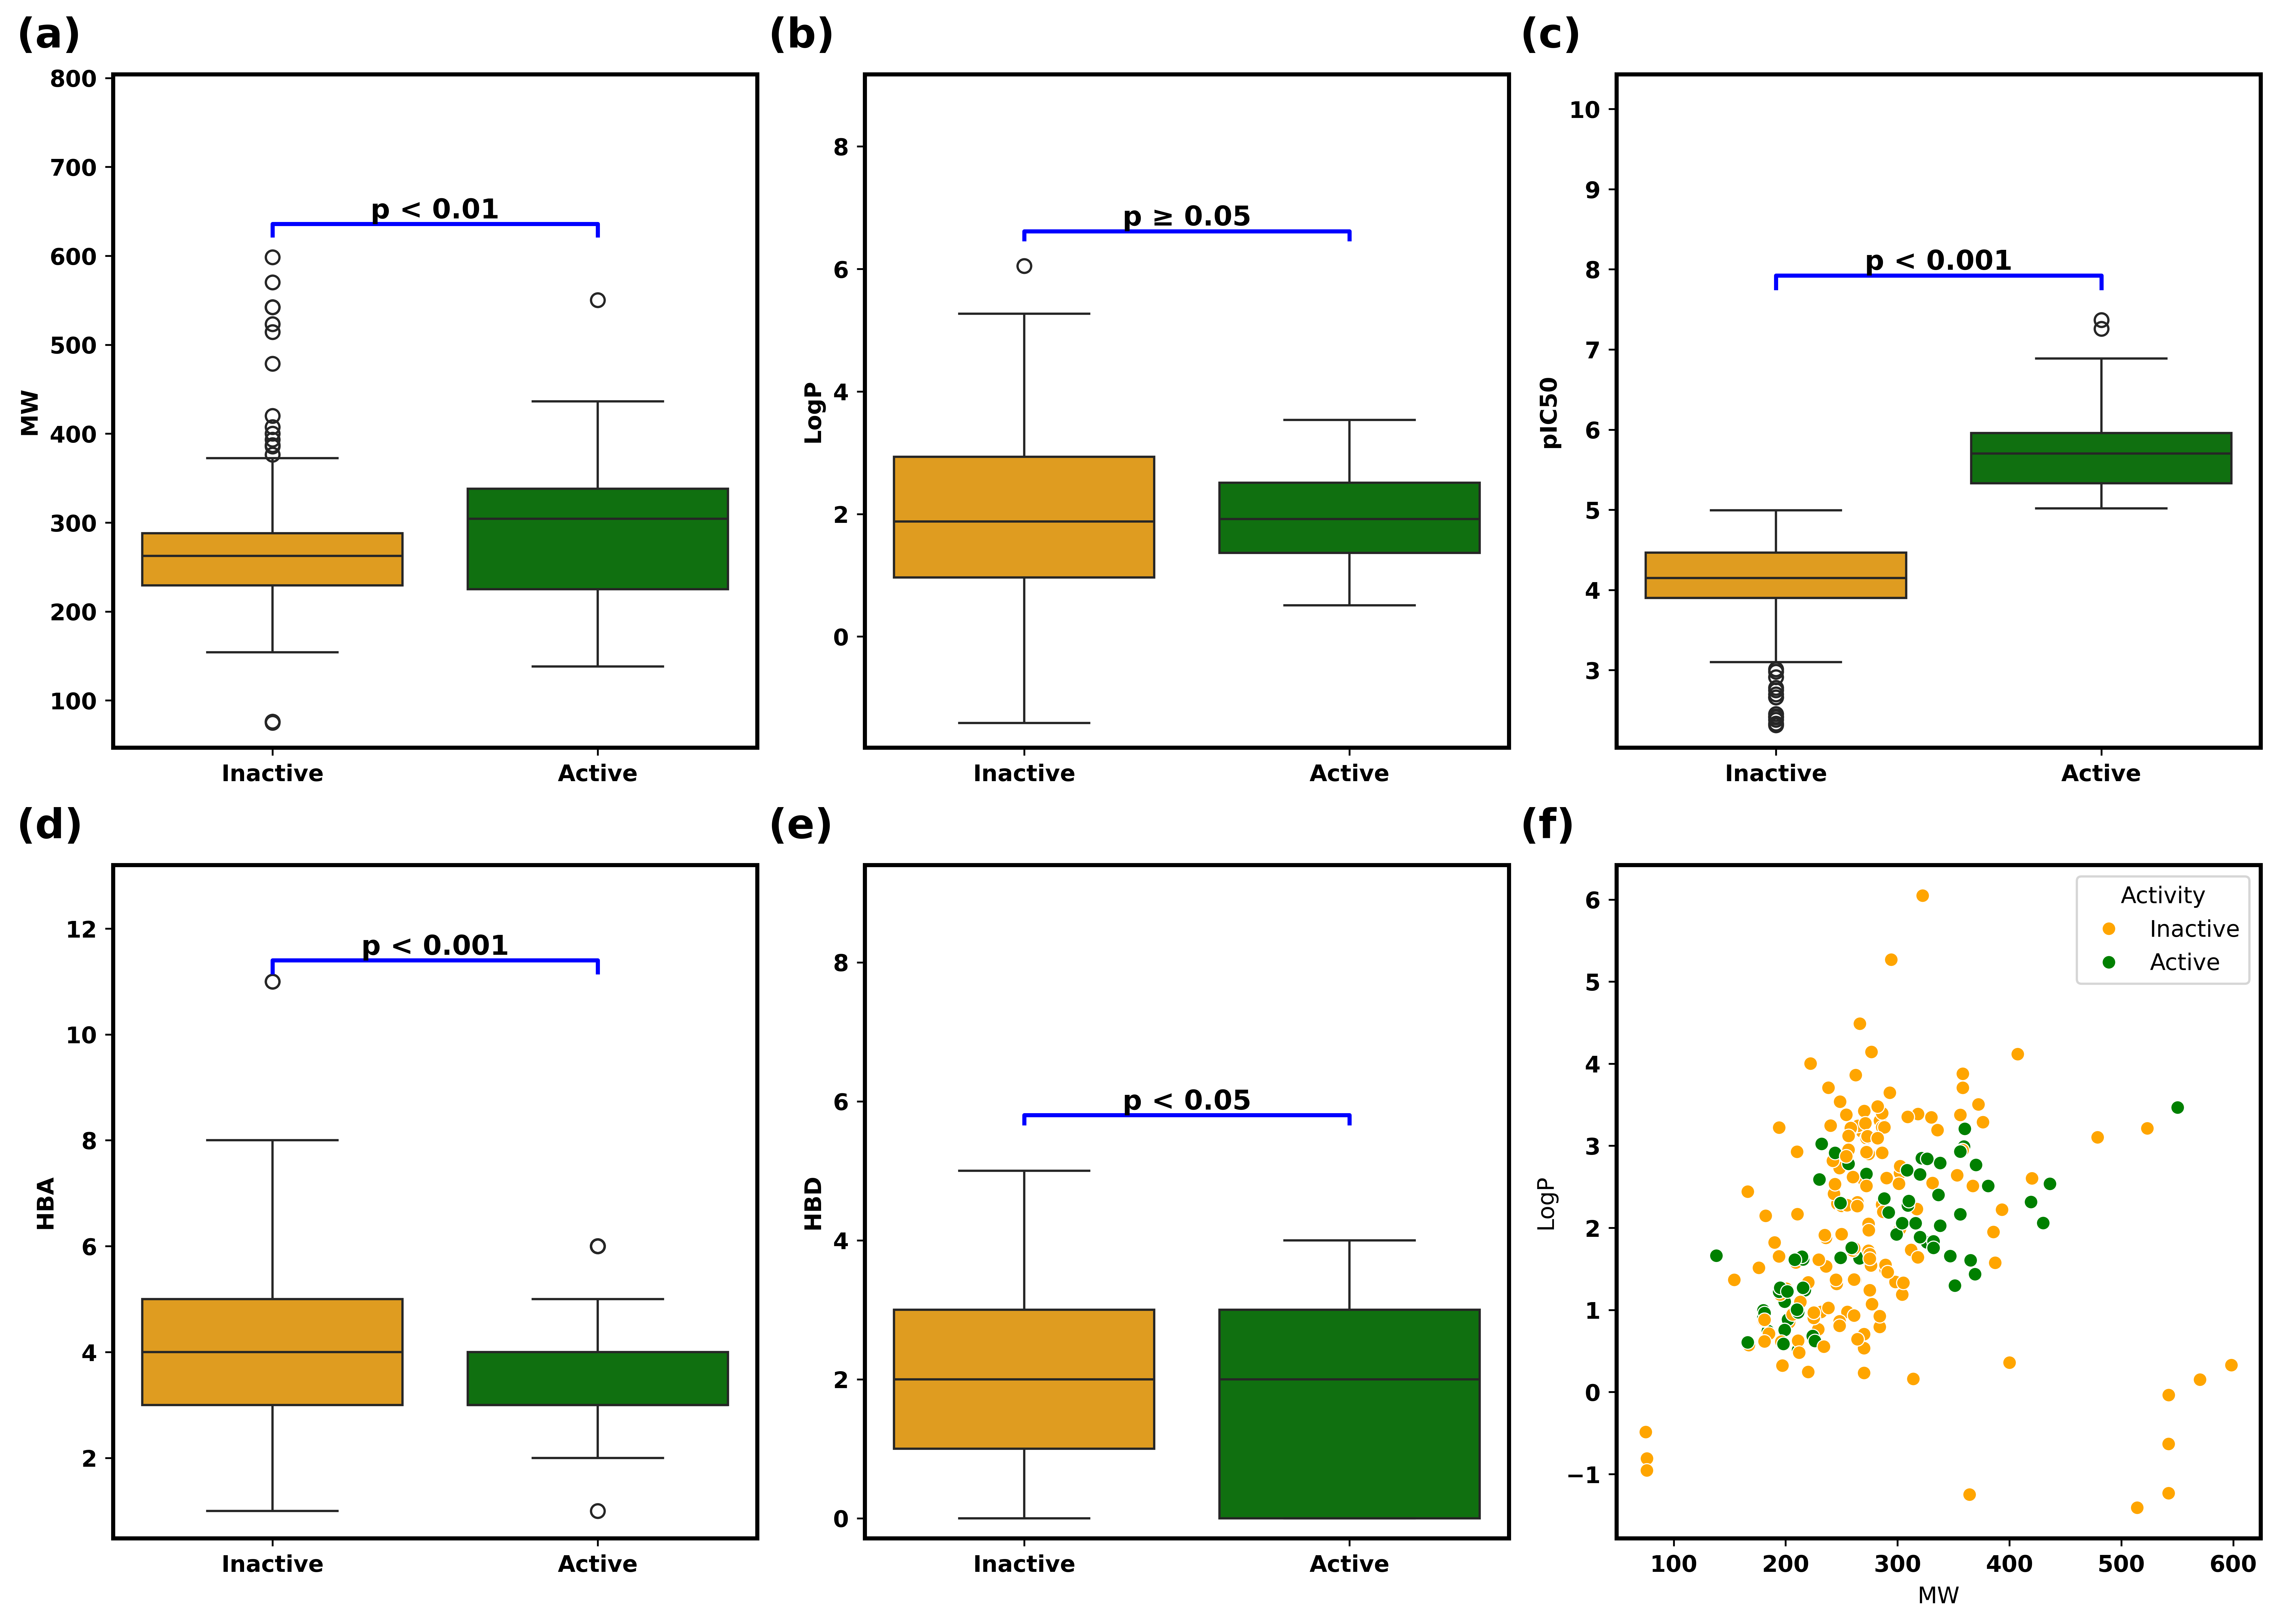
\includegraphics[width=\dimexpr\textwidth-10pt\relax]{prism-uploads/EDA_FINAL.png}};
\end{tikzpicture}
\caption[Exploratory data analysis of the curated dataset]{Exploratory data analysis of the retained \textit{H. pylori} urease inhibitor modeling cohort. The final dataset contained 351 compounds; for descriptive summary only, 133 entries were Active (pIC$_{50} \geq 5$) and 218 entries were Inactive (pIC$_{50} < 5$).}
\label{fig:eda-final}
\end{figure}

The curated compounds showed chemically diverse physicochemical profiles, reflecting the broad range of urease inhibitor chemotypes reported in the literature. The descriptor distributions in Figure~\ref{fig:eda-final} indicate that the dataset included both relatively small polar inhibitors and larger hydrophobic scaffolds, consistent with the known diversity of hydroxamate, heterocyclic, selenium-containing, and natural-product-derived urease inhibitor classes. PubChem fingerprint processing reduced the original 881 fingerprint bits to 389 after variance filtering, removing 492 low-variance features. Correlation filtering then removed 254 highly correlated features, leaving 135 fingerprint descriptors for regression modeling. Together with endpoint and identifier columns, the final processed table had dimensions of 351 compounds by 138 columns. These filtering steps reduced descriptor redundancy while retaining a chemically informative representation for pIC$_{50}$ regression.

\subsection{Baseline Model Benchmarking}

The baseline regressor screen served as an initial model-family assessment rather than a final model-selection procedure. The LazyPredict benchmark compared 41 regression algorithms with default settings on the random 80/20 split; the ten strongest completed models are shown in Table~\ref{tab:lazypredict-regression}. HistGradientBoostingRegressor gave the strongest external test performance in the benchmark (R$^2$ = 0.712; RMSE = 0.506), whereas several unstable linear or kernel methods produced negative R$^2$ values. These results supported detailed evaluation of the strongest ensemble and regularized candidates.

\begin{table}[htbp]
\centering
\scriptsize
\setlength{\tabcolsep}{4pt}
\caption[LazyPredict baseline regressor screen]{Ten strongest regressors from the LazyPredict baseline screen for pIC$_{50}$ prediction using the random train--test split, organized by descending test-set R$^2$.}
\label{tab:lazypredict-regression}
\begin{tabular}{rlrr}
\hline
Rank & Model & R$^2$ & RMSE \\
\hline
1 & HistGradientBoostingRegressor & 0.712 & 0.506 \\
2 & LassoLarsIC & 0.610 & 0.589 \\
3 & ElasticNetCV & 0.608 & 0.590 \\
4 & LassoCV & 0.607 & 0.591 \\
5 & LassoLarsCV & 0.607 & 0.591 \\
6 & RandomForestRegressor & 0.603 & 0.594 \\
7 & GradientBoostingRegressor & 0.594 & 0.601 \\
8 & BayesianRidge & 0.591 & 0.603 \\
9 & OrthogonalMatchingPursuitCV & 0.580 & 0.611 \\
10 & PoissonRegressor & 0.579 & 0.612 \\
\hline
\end{tabular}
\end{table}

The strongest baseline-screen candidates were then evaluated using the final 135 PubChem fingerprint descriptors, with five-fold cross-validation on the 280-compound training set and external evaluation on the 71-compound test set. Table~\ref{tab:final-sklearn-models} summarizes selected-model performance. HistGradientBoosting gave the best independent test performance, BayesianRidge provided the second-best test R$^2$ with comparatively strong cross-validation behavior, and the tree ensembles showed the expected trade-off between training fit and external generalization.

HistGradientBoosting retained the best independent test performance (R$^2_{test}$ = 0.712; RMSE$_{test}$ = 0.506; MAE$_{test}$ = 0.375), whereas GradientBoosting gave the highest cross-validated Q$^2$ (0.606). Relative to RandomForest, HistGradientBoosting improved independent test R$^2$ by 0.109 absolute units, corresponding to an approximately 18\% relative gain, while reducing RMSE$_{test}$ from 0.594 to 0.506. RandomForest showed the highest training R$^2$ (0.934) but lower Q$^2$ and test R$^2$ values, consistent with stronger overfitting relative to the boosting and Bayesian models. HistGradientBoosting was therefore retained as the strongest baseline regression model in the current analysis. The corresponding observed-versus-predicted parity plots are shown in Figure~\ref{fig:parity-plots}.

\begin{table}[htbp]
\centering
\scriptsize
\setlength{\tabcolsep}{3pt}
\caption[External performance of selected regressors]{External performance of selected regressors using 135 retained PubChem fingerprint descriptors.}
\label{tab:final-sklearn-models}
\begin{tabular}{lrrrrrrrrr}
\hline
Model & R$^2_{train}$ & Q$^2_{CV}$ & R$^2_{test}$ & RMSE$_{train}$ & RMSE$_{CV}$ & RMSE$_{test}$ & MAE$_{train}$ & MAE$_{CV}$ & MAE$_{test}$ \\
\hline
HistGradientBoosting & 0.794 & 0.538 & 0.712 & 0.433 & 0.647 & 0.506 & 0.299 & 0.470 & 0.375 \\
BayesianRidge & 0.786 & 0.595 & 0.643 & 0.440 & 0.606 & 0.563 & 0.323 & 0.447 & 0.431 \\
LassoLarsIC & 0.813 & 0.574 & 0.619 & 0.412 & 0.622 & 0.582 & 0.301 & 0.451 & 0.432 \\
RandomForest & 0.934 & 0.572 & 0.603 & 0.244 & 0.623 & 0.594 & 0.169 & 0.446 & 0.437 \\
GradientBoosting & 0.872 & 0.606 & 0.594 & 0.341 & 0.598 & 0.601 & 0.255 & 0.438 & 0.446 \\
\hline
\end{tabular}
\end{table}

\begin{figure}[p]
\centering
\scriptsize
\setlength{\tabcolsep}{3pt}
\renewcommand{\arraystretch}{0.78}
\begin{tabular}{cc}
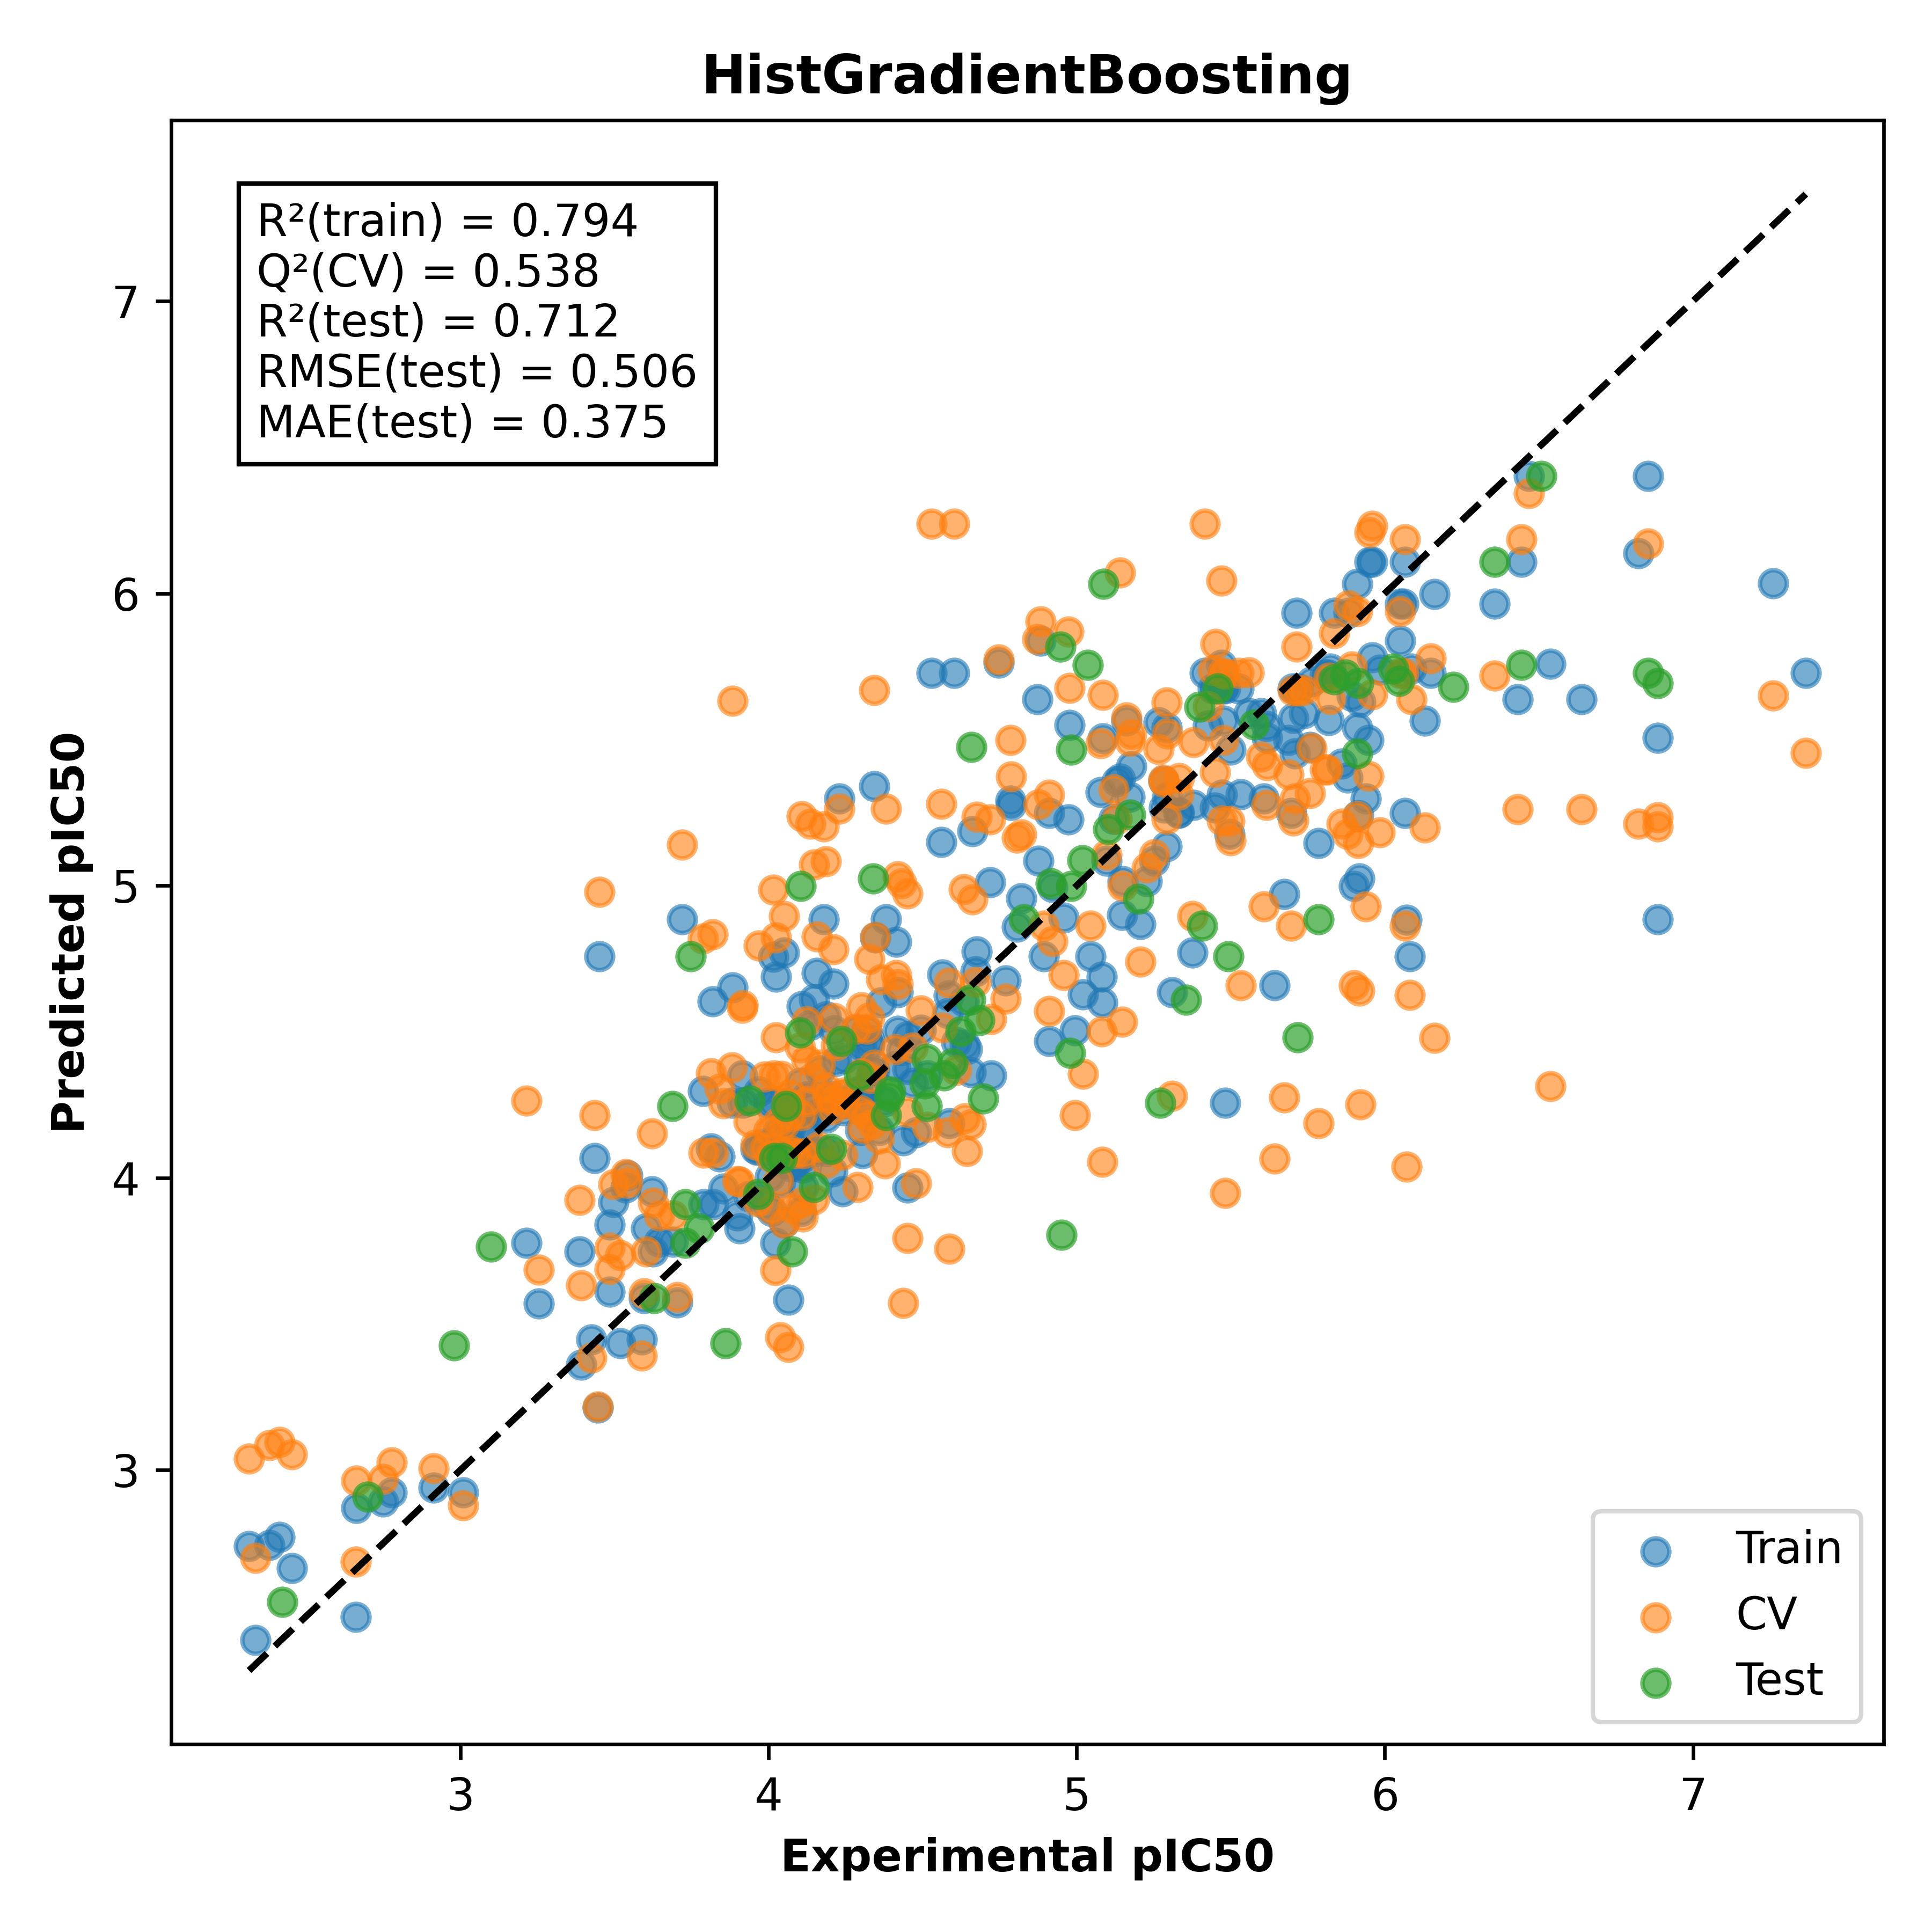
\includegraphics[width=0.41\textwidth]{prism-uploads/HistGradientBoosting_Parity.png} &
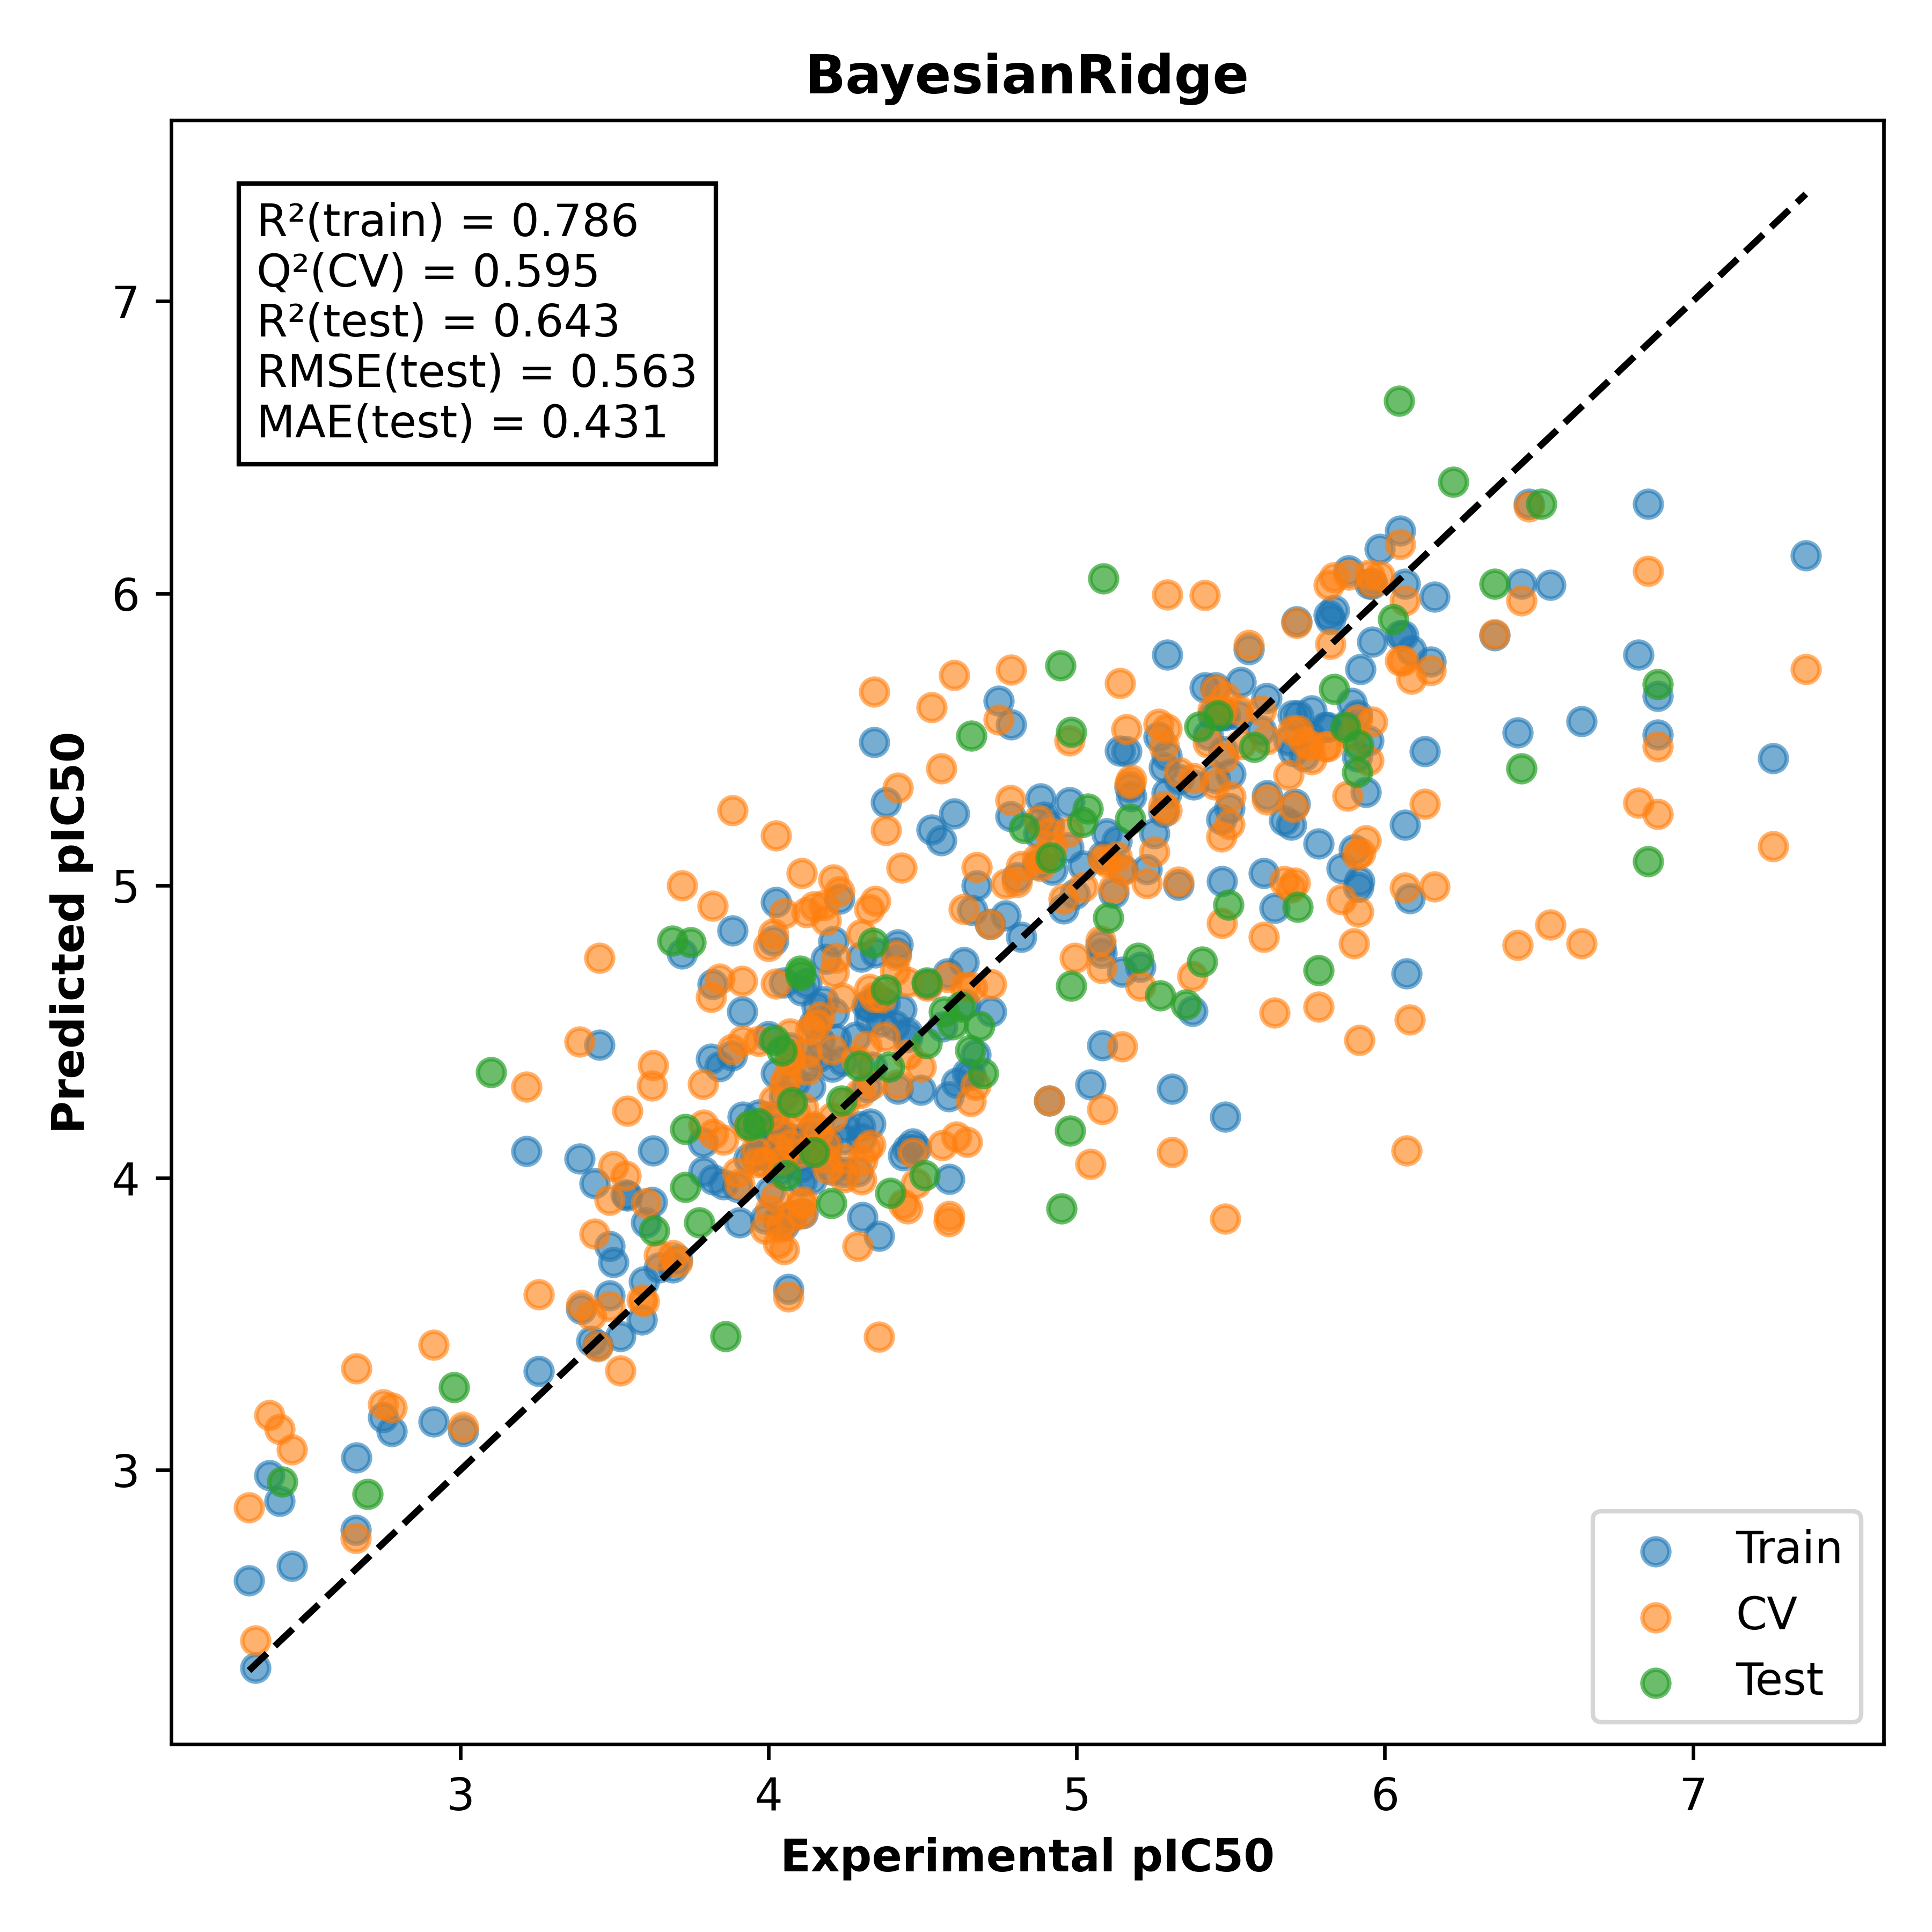
\includegraphics[width=0.41\textwidth]{prism-uploads/BayesianRidge_Parity.png} \\
(a) HistGradientBoosting & (b) BayesianRidge \\[3pt]
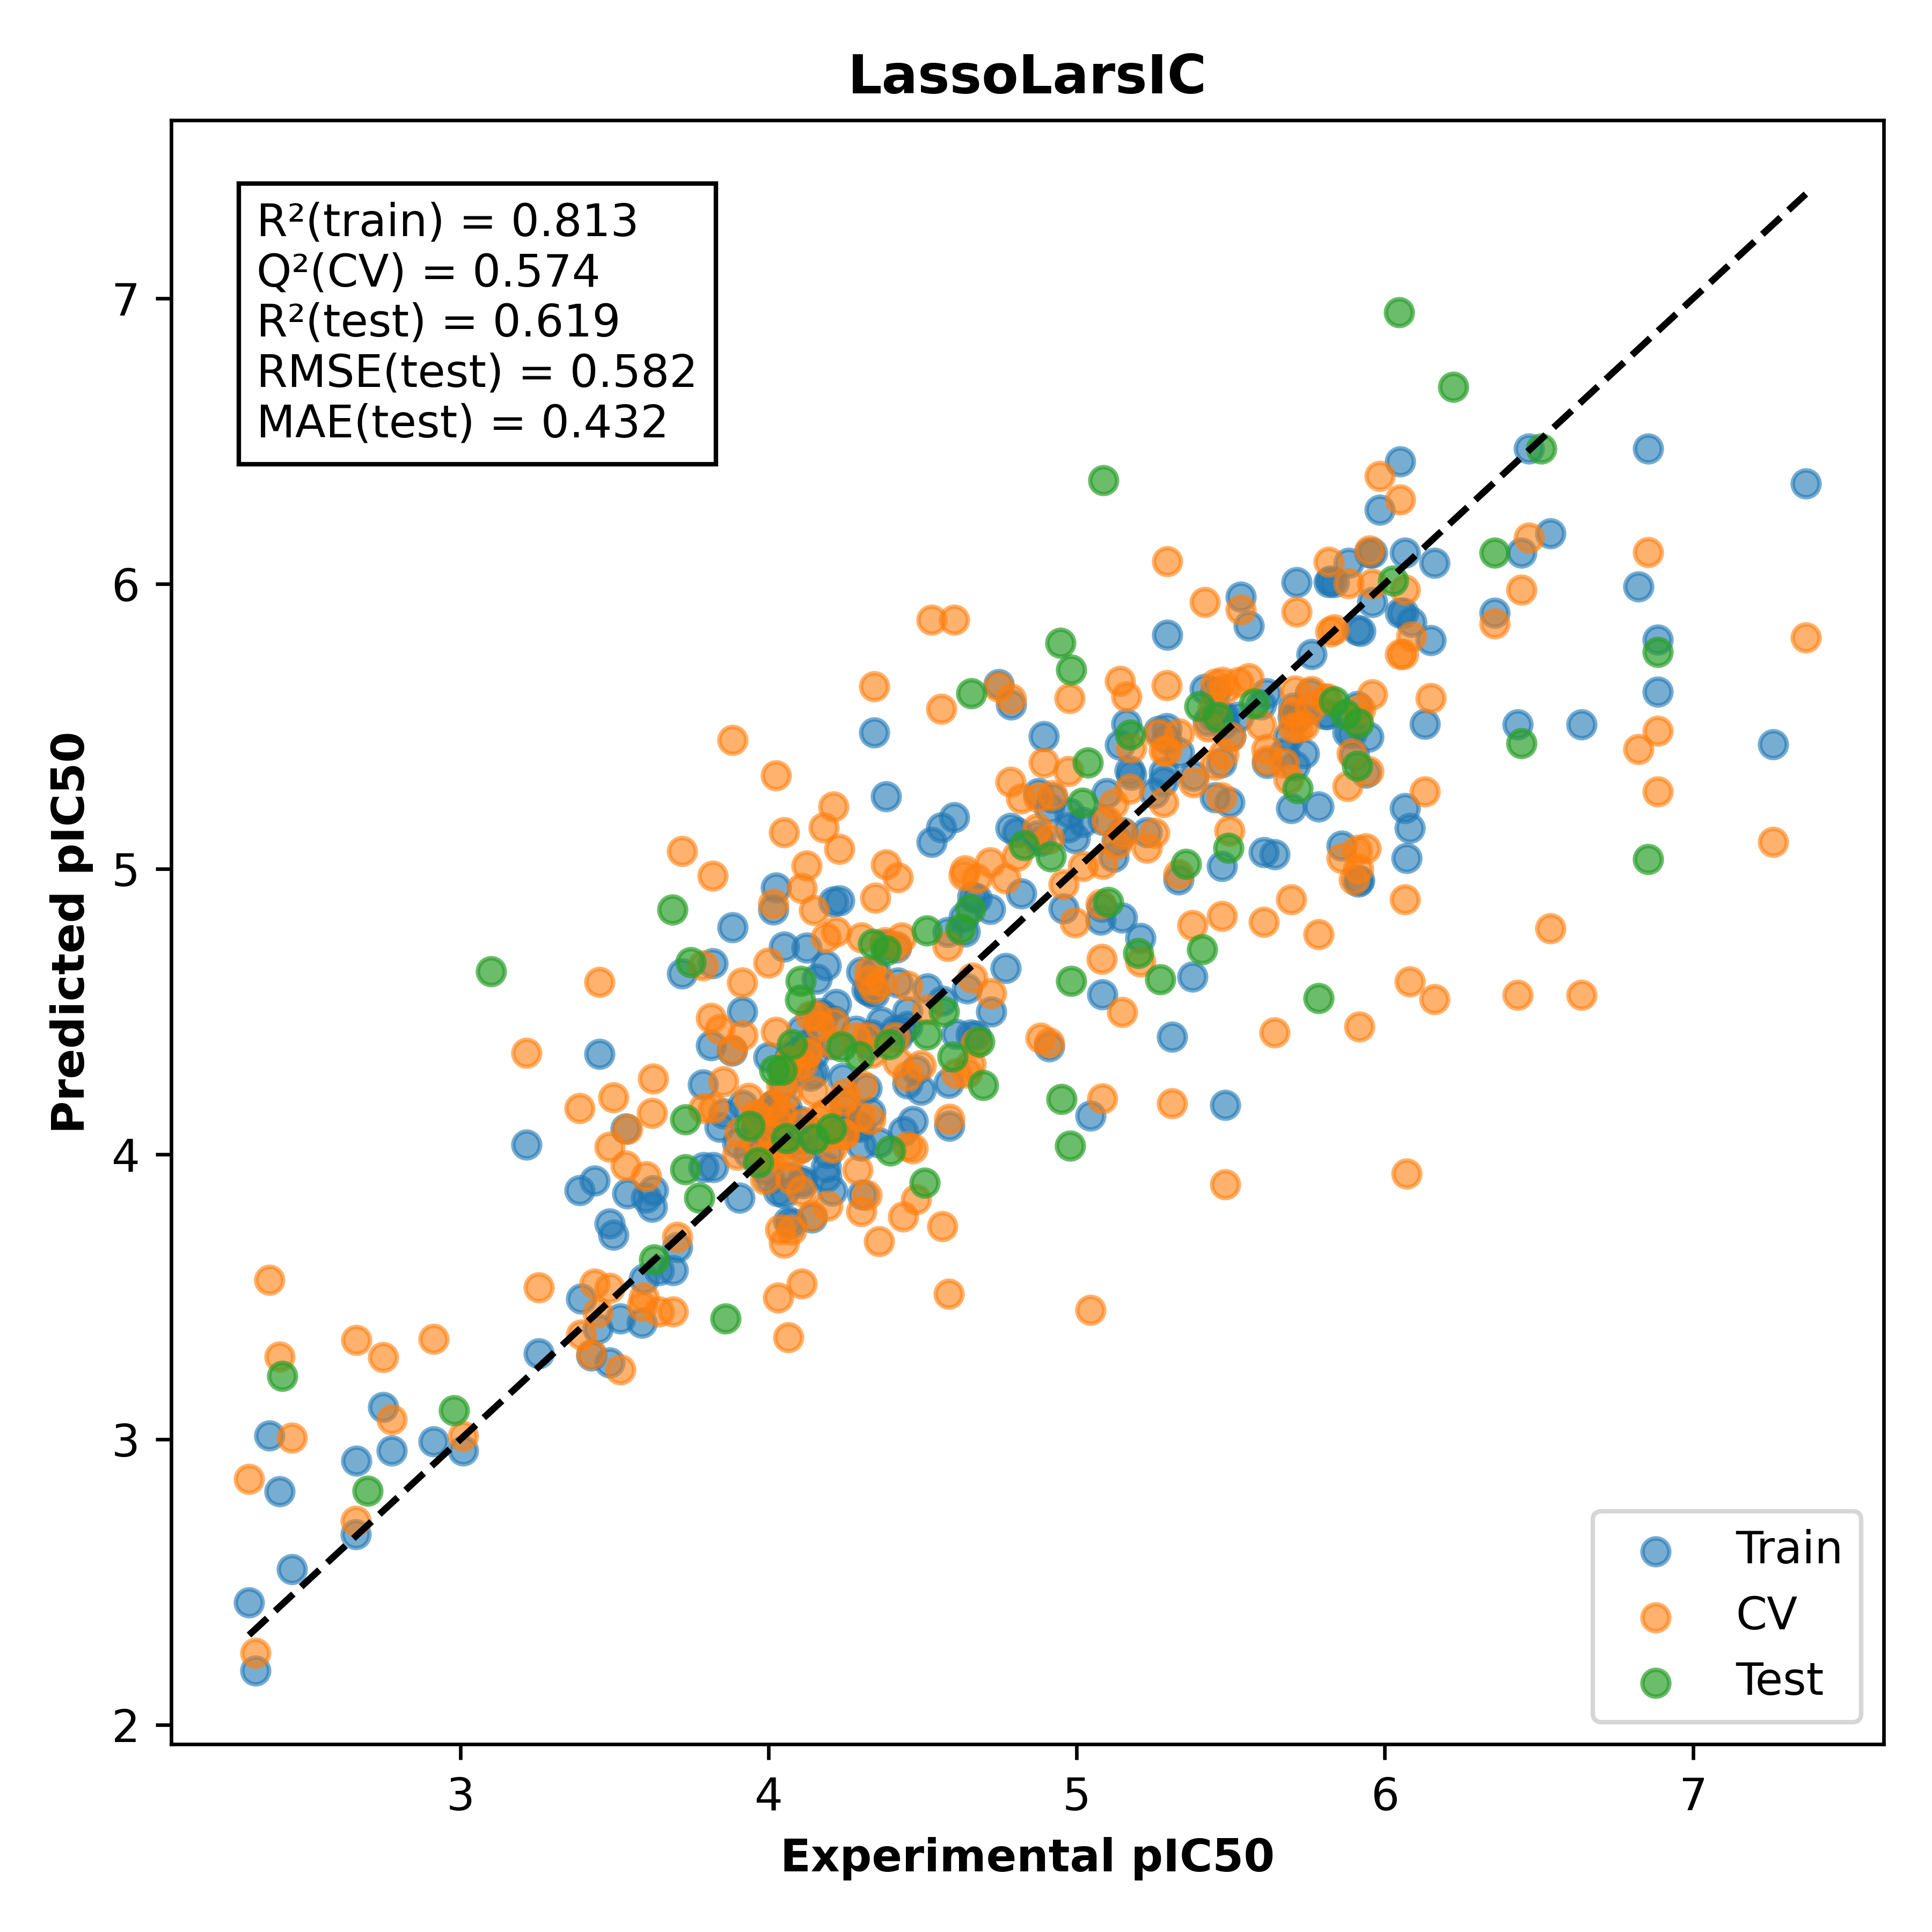
\includegraphics[width=0.41\textwidth]{prism-uploads/LassoLarsIC_Parity.png} &
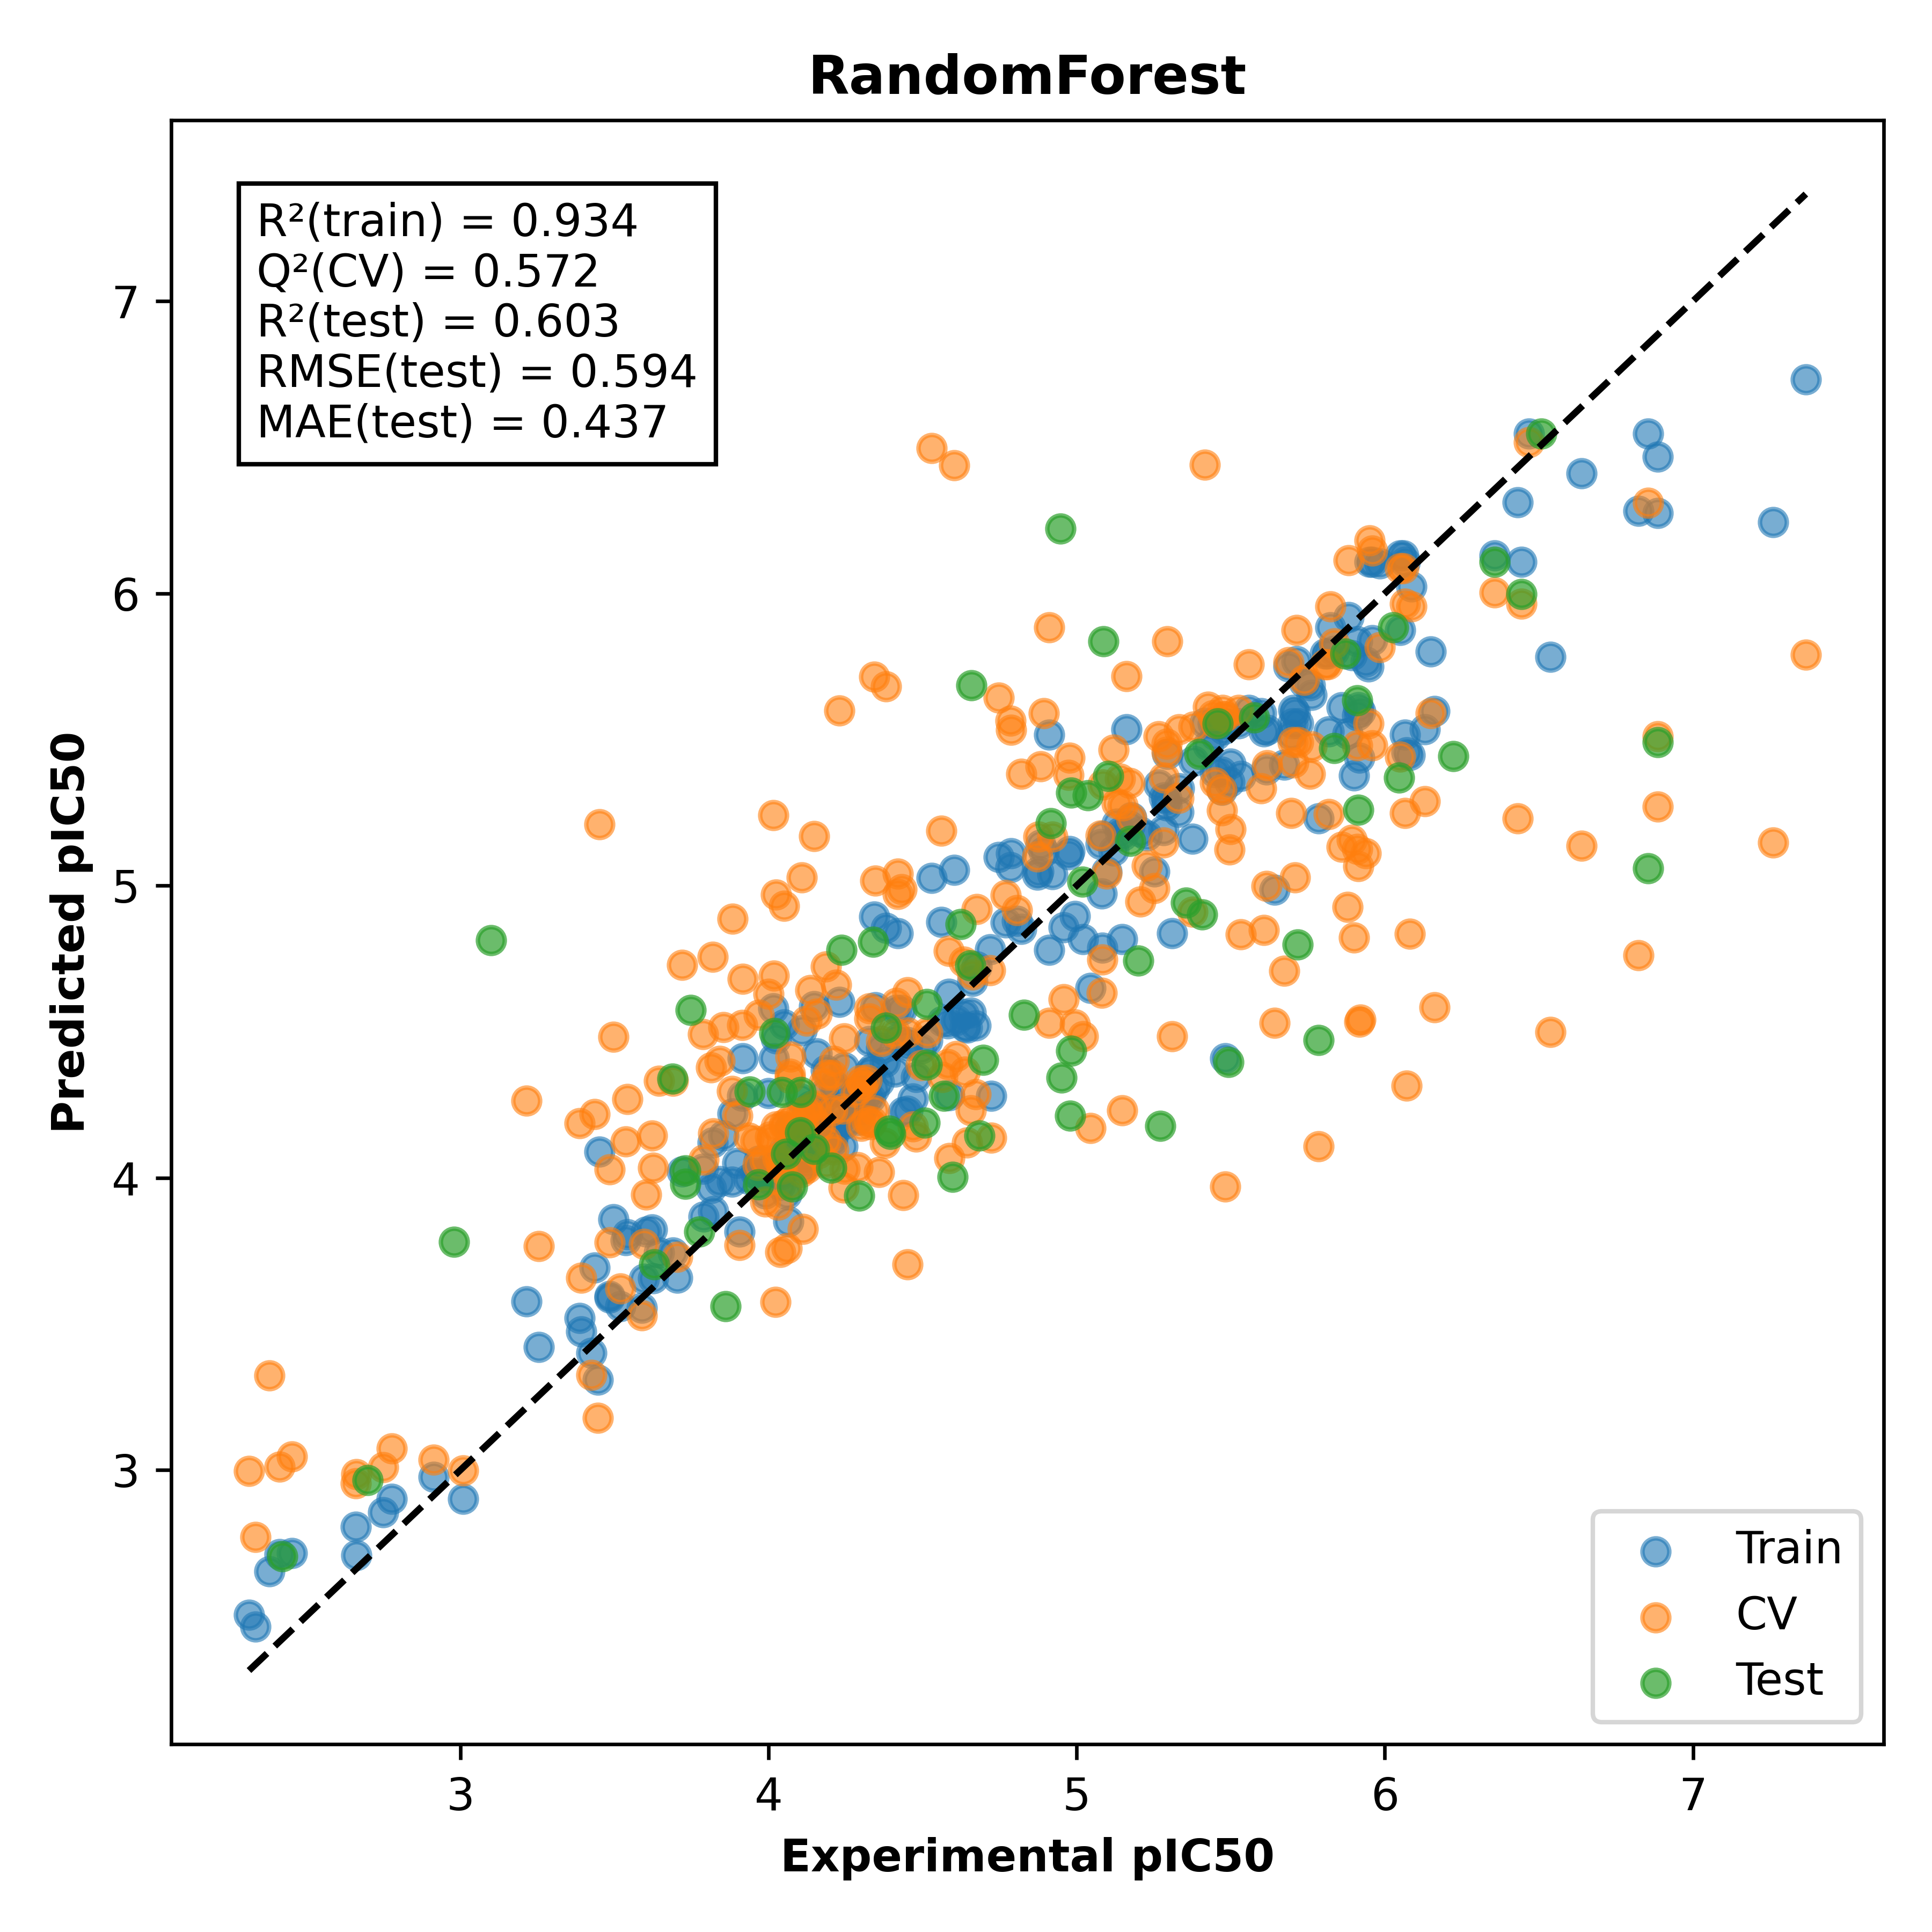
\includegraphics[width=0.41\textwidth]{prism-uploads/RandomForest_Parity.png} \\
(c) LassoLarsIC & (d) RandomForest \\[3pt]
\multicolumn{2}{c}{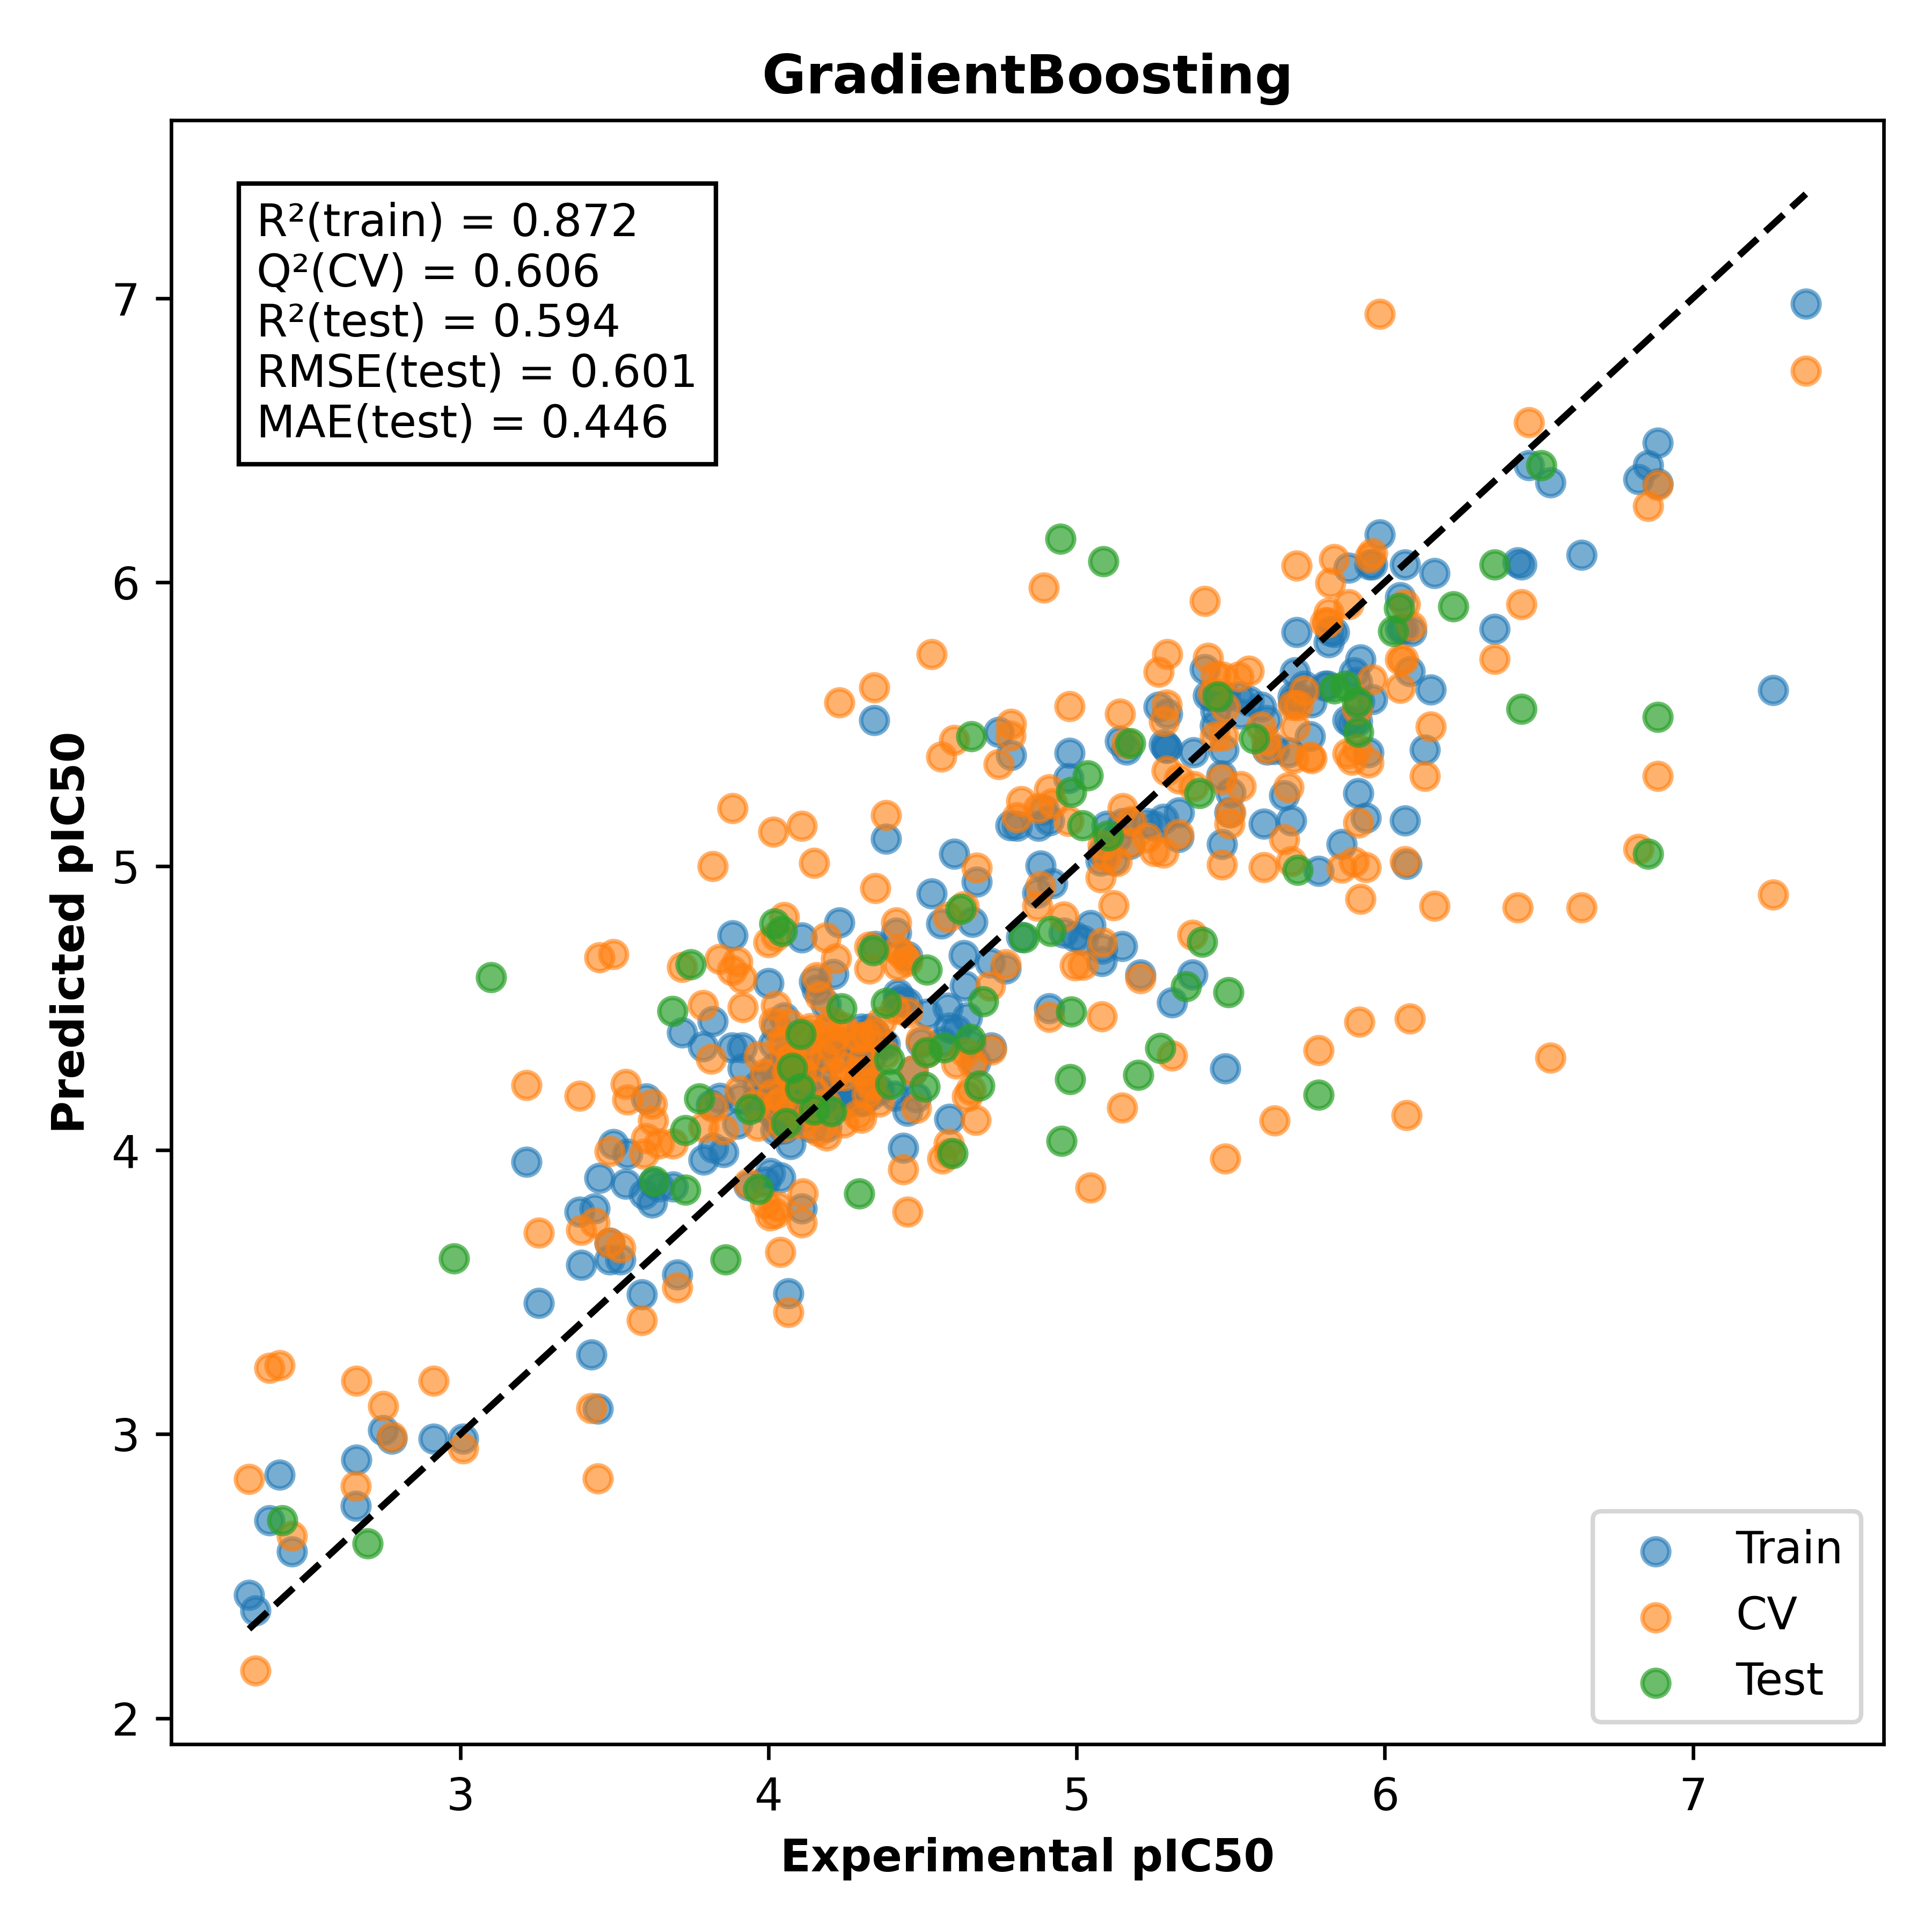
\includegraphics[width=0.41\textwidth]{prism-uploads/GradientBoosting_Parity.png}} \\
\multicolumn{2}{c}{(e) GradientBoosting} \\
\end{tabular}
\caption[Observed-versus-predicted parity plots]{Observed-versus-predicted pIC$_{50}$ parity plots for the five selected scikit-learn regression models retrained using the 135 retained PubChem fingerprint descriptors.}
\label{fig:parity-plots}
\end{figure}

OECD-style external validation provided regression-consistency checks beyond ordinary test-set R$^2$ for the five retrained scikit-learn models. Table~\ref{tab:oecd-validation} reports these statistics for the selected models. HistGradientBoosting showed the strongest external validation profile, with $R^2_{ext}$ = 0.714 and PASS\_OECD = True. BayesianRidge, LassoLarsIC, and RandomForest also passed the implemented OECD-style checks, whereas GradientBoosting did not pass despite having the highest Q$^2_{CV}$ among the selected models. This contrast indicates that internal cross-validation performance did not fully predict external validation robustness.

\begin{table}[htbp]
\centering
\scriptsize
\setlength{\tabcolsep}{3pt}
\caption[OECD-style external validation statistics]{OECD-style external validation statistics for the selected scikit-learn regression models.}
\label{tab:oecd-validation}
\resizebox{\textwidth}{!}{%
\begin{tabular}{lrrrrrrrl}
\hline
Model & Q$^2_{CV}$ & R$^2_{test}$ & R$^2_{ext}$ & $k$ & $k'$ & $R^2_0$ & $R'^2_0$ & PASS\_OECD \\
\hline
HistGradientBoosting & 0.538 & 0.712 & 0.714 & 1.015 & 0.975 & 0.718 & 0.626 & True \\
BayesianRidge & 0.595 & 0.643 & 0.645 & 1.005 & 0.982 & 0.644 & 0.473 & True \\
LassoLarsIC & 0.574 & 0.619 & 0.622 & 0.996 & 0.989 & 0.620 & 0.504 & True \\
RandomForest & 0.572 & 0.603 & 0.605 & 1.017 & 0.969 & 0.610 & 0.420 & True \\
GradientBoosting & 0.606 & 0.594 & 0.596 & 1.017 & 0.969 & 0.601 & 0.410 & False \\
\hline
\end{tabular}%
}
\end{table}

Y-randomization served as a negative-control analysis in which pIC$_{50}$ response values were randomized before refitting the selected models. Table~\ref{tab:y-randomization} summarizes the mean and standard deviation of randomized-model performance. All selected models produced negative mean randomized-test R$^2$ values, whereas RMSE$_{test}$ and MAE$_{test}$ increased relative to the non-randomized models. Thus, the external performance reported in Table~\ref{tab:final-sklearn-models} was not reproduced after response randomization.

\begin{table}[htbp]
\centering
\scriptsize
\setlength{\tabcolsep}{3pt}
\caption[Y-randomization summary]{Y-randomization summary for selected regressors after response-value randomization.}
\label{tab:y-randomization}
\resizebox{\textwidth}{!}{%
\begin{tabular}{lrrrrrrrr}
\hline
Model & R$^2_{train}$ mean & R$^2_{train}$ std & R$^2_{test}$ mean & R$^2_{test}$ std & RMSE$_{test}$ mean & RMSE$_{test}$ std & MAE$_{test}$ mean & MAE$_{test}$ std \\
\hline
BayesianRidge & 0.014 & 0.025 & -0.011 & 0.028 & 0.948 & 0.013 & 0.756 & 0.011 \\
GradientBoosting & 0.501 & 0.031 & -0.277 & 0.160 & 1.063 & 0.066 & 0.844 & 0.055 \\
HistGradientBoosting & 0.384 & 0.031 & -0.197 & 0.140 & 1.030 & 0.060 & 0.824 & 0.052 \\
LassoLarsIC & 0.023 & 0.045 & -0.013 & 0.050 & 0.948 & 0.022 & 0.757 & 0.022 \\
RandomForest & 0.746 & 0.022 & -0.250 & 0.140 & 1.052 & 0.059 & 0.839 & 0.053 \\
\hline
\end{tabular}%
}
\end{table}

\subsection{Chemical Determinants of Predicted Potency}

SHAP analysis identified the PubChem fingerprint descriptors that contributed most strongly to predictions from the final HistGradientBoosting QSAR model. The ten highest-ranked descriptors were dominated by heteroatom, carbonyl-containing, aliphatic, halogenated, oxygenated-chain, aromatic-carbon, and diamine-like fingerprint definitions (Table~\ref{tab:top10-shap-features}). PubChem\_14, corresponding to the presence of at least one nitrogen atom, had the largest mean absolute SHAP value, followed by carbonyl-chain and amide-like patterns represented by PubChem\_535 and PubChem\_646. The attribution profile was therefore concentrated in chemically interpretable fingerprint patterns rather than distributed uniformly across all 135 retained descriptors.

Figure~\ref{fig:shap-panels}a ranks the top ten descriptors by mean absolute SHAP value, and Figure~\ref{fig:shap-panels}b shows the direction and dispersion of feature effects across individual compounds. Positive SHAP values correspond to descriptor-associated increases in predicted pIC$_{50}$ relative to the model baseline, whereas negative SHAP values correspond to descriptor-associated decreases. For binary PubChem descriptors, separation between compounds with and without a fingerprint bit shows how descriptor presence or absence influenced prediction magnitude across the training set. These plots support quantitative descriptor interpretation without assigning unsupported causal pharmacophore status to individual fingerprint identifiers.

\begin{table}[htbp]
\centering
\scriptsize
\setlength{\tabcolsep}{4pt}
\caption[Top ten SHAP-ranked PubChem fingerprint descriptors]{Top ten PubChem fingerprint descriptors identified by SHAP analysis of the final HistGradientBoosting QSAR model. Descriptors are ranked according to mean absolute SHAP values calculated across the 280-compound training set; interpreted definitions were obtained from the PubChem fingerprint dictionary.}
\label{tab:top10-shap-features}
\resizebox{\textwidth}{!}{%
\begin{tabular}{rrlrl}
\hline
Rank & Bit & Feature & MeanAbsSHAP & PubChem fingerprint definition \\
\hline
1 & 14 & PubChem\_14 & 0.192172 & $\geq$ 1 N \\
2 & 535 & PubChem\_535 & 0.149673 & O=C-C-C \\
3 & 646 & PubChem\_646 & 0.147297 & O=C-N-C-[\#1] \\
4 & 374 & PubChem\_374 & 0.146007 & C($\sim$H)($\sim$H)($\sim$H) \\
5 & 700 & PubChem\_700 & 0.101705 & O-C-C-C-C-C-O-C \\
6 & 439 & PubChem\_439 & 0.088942 & C(-C)(-N)(=O) \\
7 & 37 & PubChem\_37 & 0.076231 & $\geq$ 1 Cl \\
8 & 663 & PubChem\_663 & 0.068910 & O-C-C-O-[\#1] \\
9 & 385 & PubChem\_385 & 0.061213 & C(:C)(:C)(:C) \\
10 & 569 & PubChem\_569 & 0.050342 & N-C-C-N \\
\hline
\end{tabular}%
}
\end{table}

\begin{figure}[p]
\centering
\scriptsize
\begin{tikzpicture}
\node[draw=black, rounded corners=8pt, line width=0.8pt, inner sep=5pt] {
\begin{tabular}{c}
\includegraphics[width=0.745\textwidth, keepaspectratio]{prism-uploads/SHAP_BAR_TOP10_WHITE.png} \\
(a) SHAP summary bar plot \\[2pt]
\includegraphics[width=0.745\textwidth, keepaspectratio]{prism-uploads/SHAP_BEESWARM_TOP10_WHITE.png} \\
(b) SHAP beeswarm plot \\
\end{tabular}
};
\end{tikzpicture}
\caption[SHAP interpretation of the final HistGradientBoosting QSAR model]{SHAP interpretation of the final HistGradientBoosting QSAR model. Panel (a) shows the global importance ranking of the ten most influential PubChem fingerprint descriptors based on mean absolute SHAP values. Panel (b) shows the magnitude and direction of descriptor contributions to predicted pIC$_{50}$ values across the training compounds.}
\label{fig:shap-panels}
\end{figure}

Fingerprint enrichment analysis was used as an additional descriptive check on the top SHAP-ranked PubChem fingerprint descriptors (Figure~\ref{fig:fingerprint-enrichment}). The analysis compared the percentage of active and inactive compounds containing each fingerprint pattern, using the same activity threshold applied only for dataset description. Several SHAP-relevant descriptors were more frequent among active compounds, including PubChem\_14 (95.3\% active versus 67.8\% inactive), PubChem\_439 (86.8\% versus 51.1\%), PubChem\_535 (71.7\% versus 52.9\%), PubChem\_385 (43.4\% versus 10.9\%), PubChem\_37 (26.4\% versus 16.7\%), and PubChem\_569 (18.9\% versus 9.8\%). In contrast, PubChem\_374, PubChem\_646, PubChem\_700, and PubChem\_663 were more frequent among inactive compounds. These enrichment patterns complement the SHAP results by showing how often the influential fingerprint bits occur in each descriptive activity group, although frequency enrichment alone should not be interpreted as causal evidence of potency.

\begin{figure}[htbp]
\centering
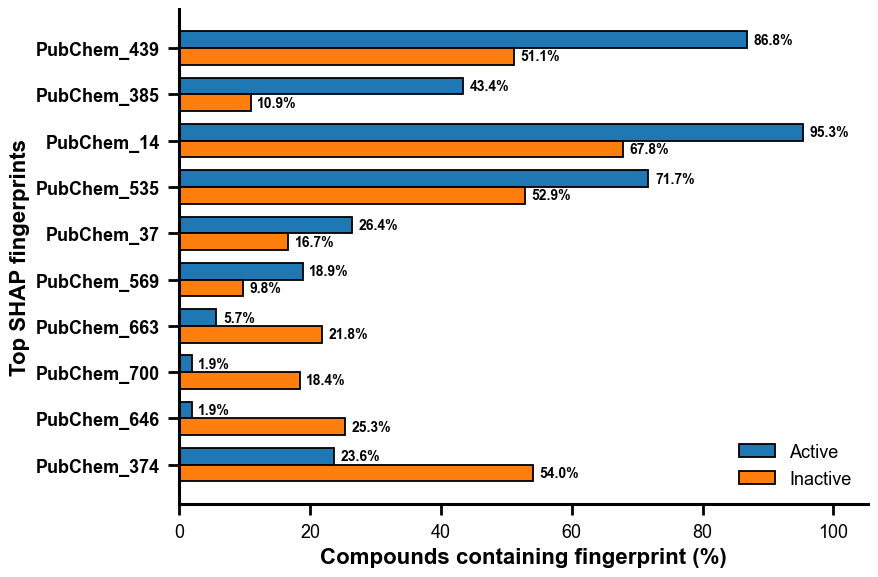
\includegraphics[width=0.92\textwidth, keepaspectratio]{prism-uploads/image.png}
\caption[Fingerprint enrichment among active and inactive compounds]{Enrichment analysis of the top SHAP-ranked PubChem fingerprint descriptors in the curated dataset. Bars show the percentage of active and inactive compounds containing each fingerprint bit. Activity grouping was used only for descriptive interpretation and not as the machine learning endpoint.}
\label{fig:fingerprint-enrichment}
\end{figure}

\begin{figure}[htbp]
\centering
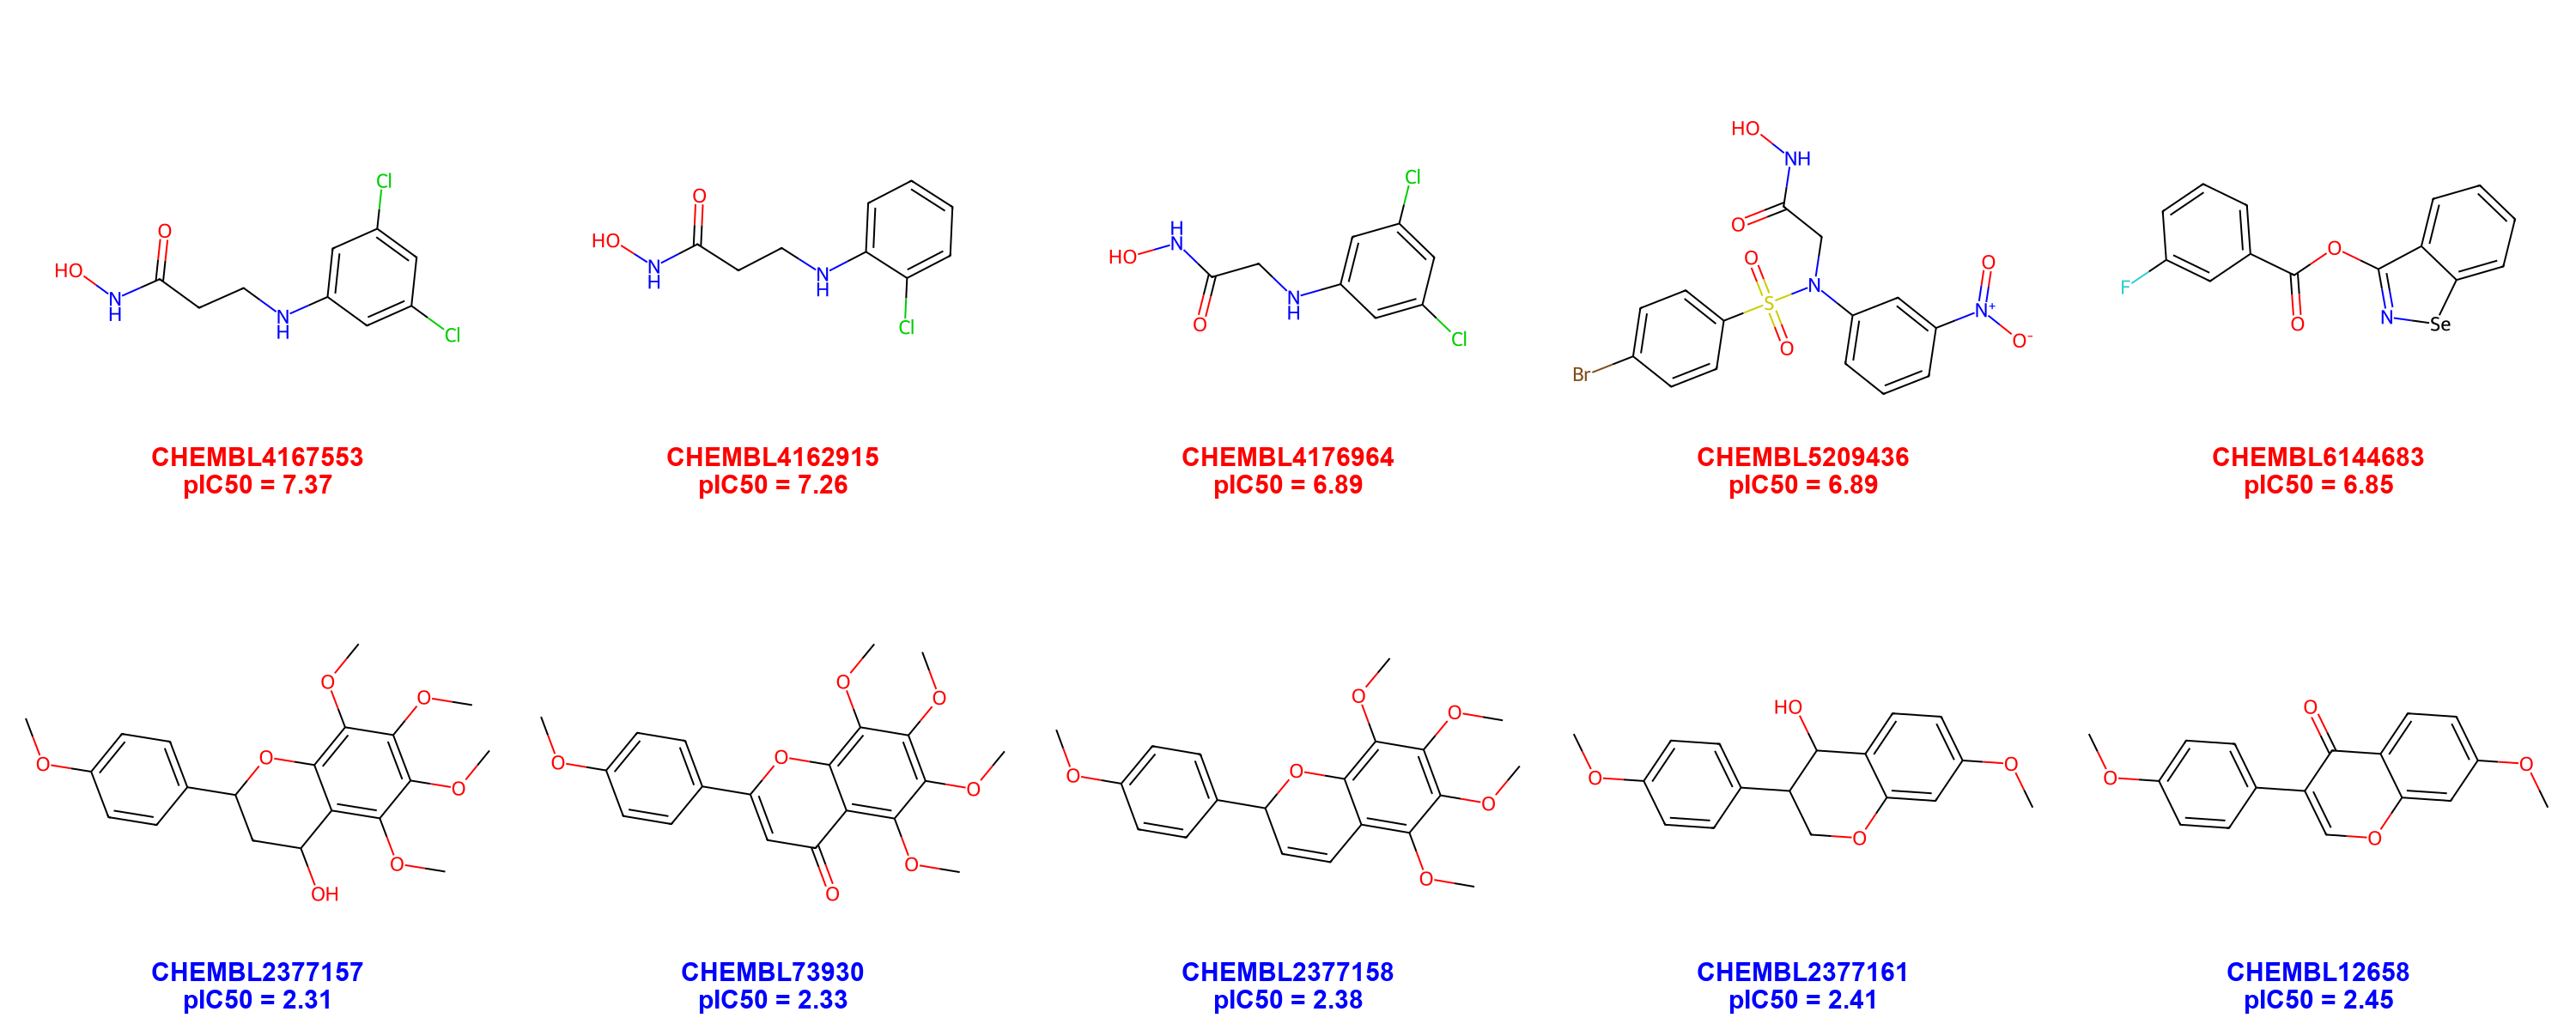
\includegraphics[width=0.98\textwidth, keepaspectratio]{prism-uploads/image_2.png}
\caption[Representative high- and low-potency urease inhibitors]{Representative chemical structures from the curated \textit{H. pylori} urease inhibitor dataset. Red labels indicate higher-potency compounds with larger pIC$_{50}$ values, whereas blue labels indicate lower-potency compounds with smaller pIC$_{50}$ values.}
\label{fig:representative-potency-structures}
\end{figure}

\begin{figure}[p]
\centering
\scriptsize
\begin{tabular}{cc}
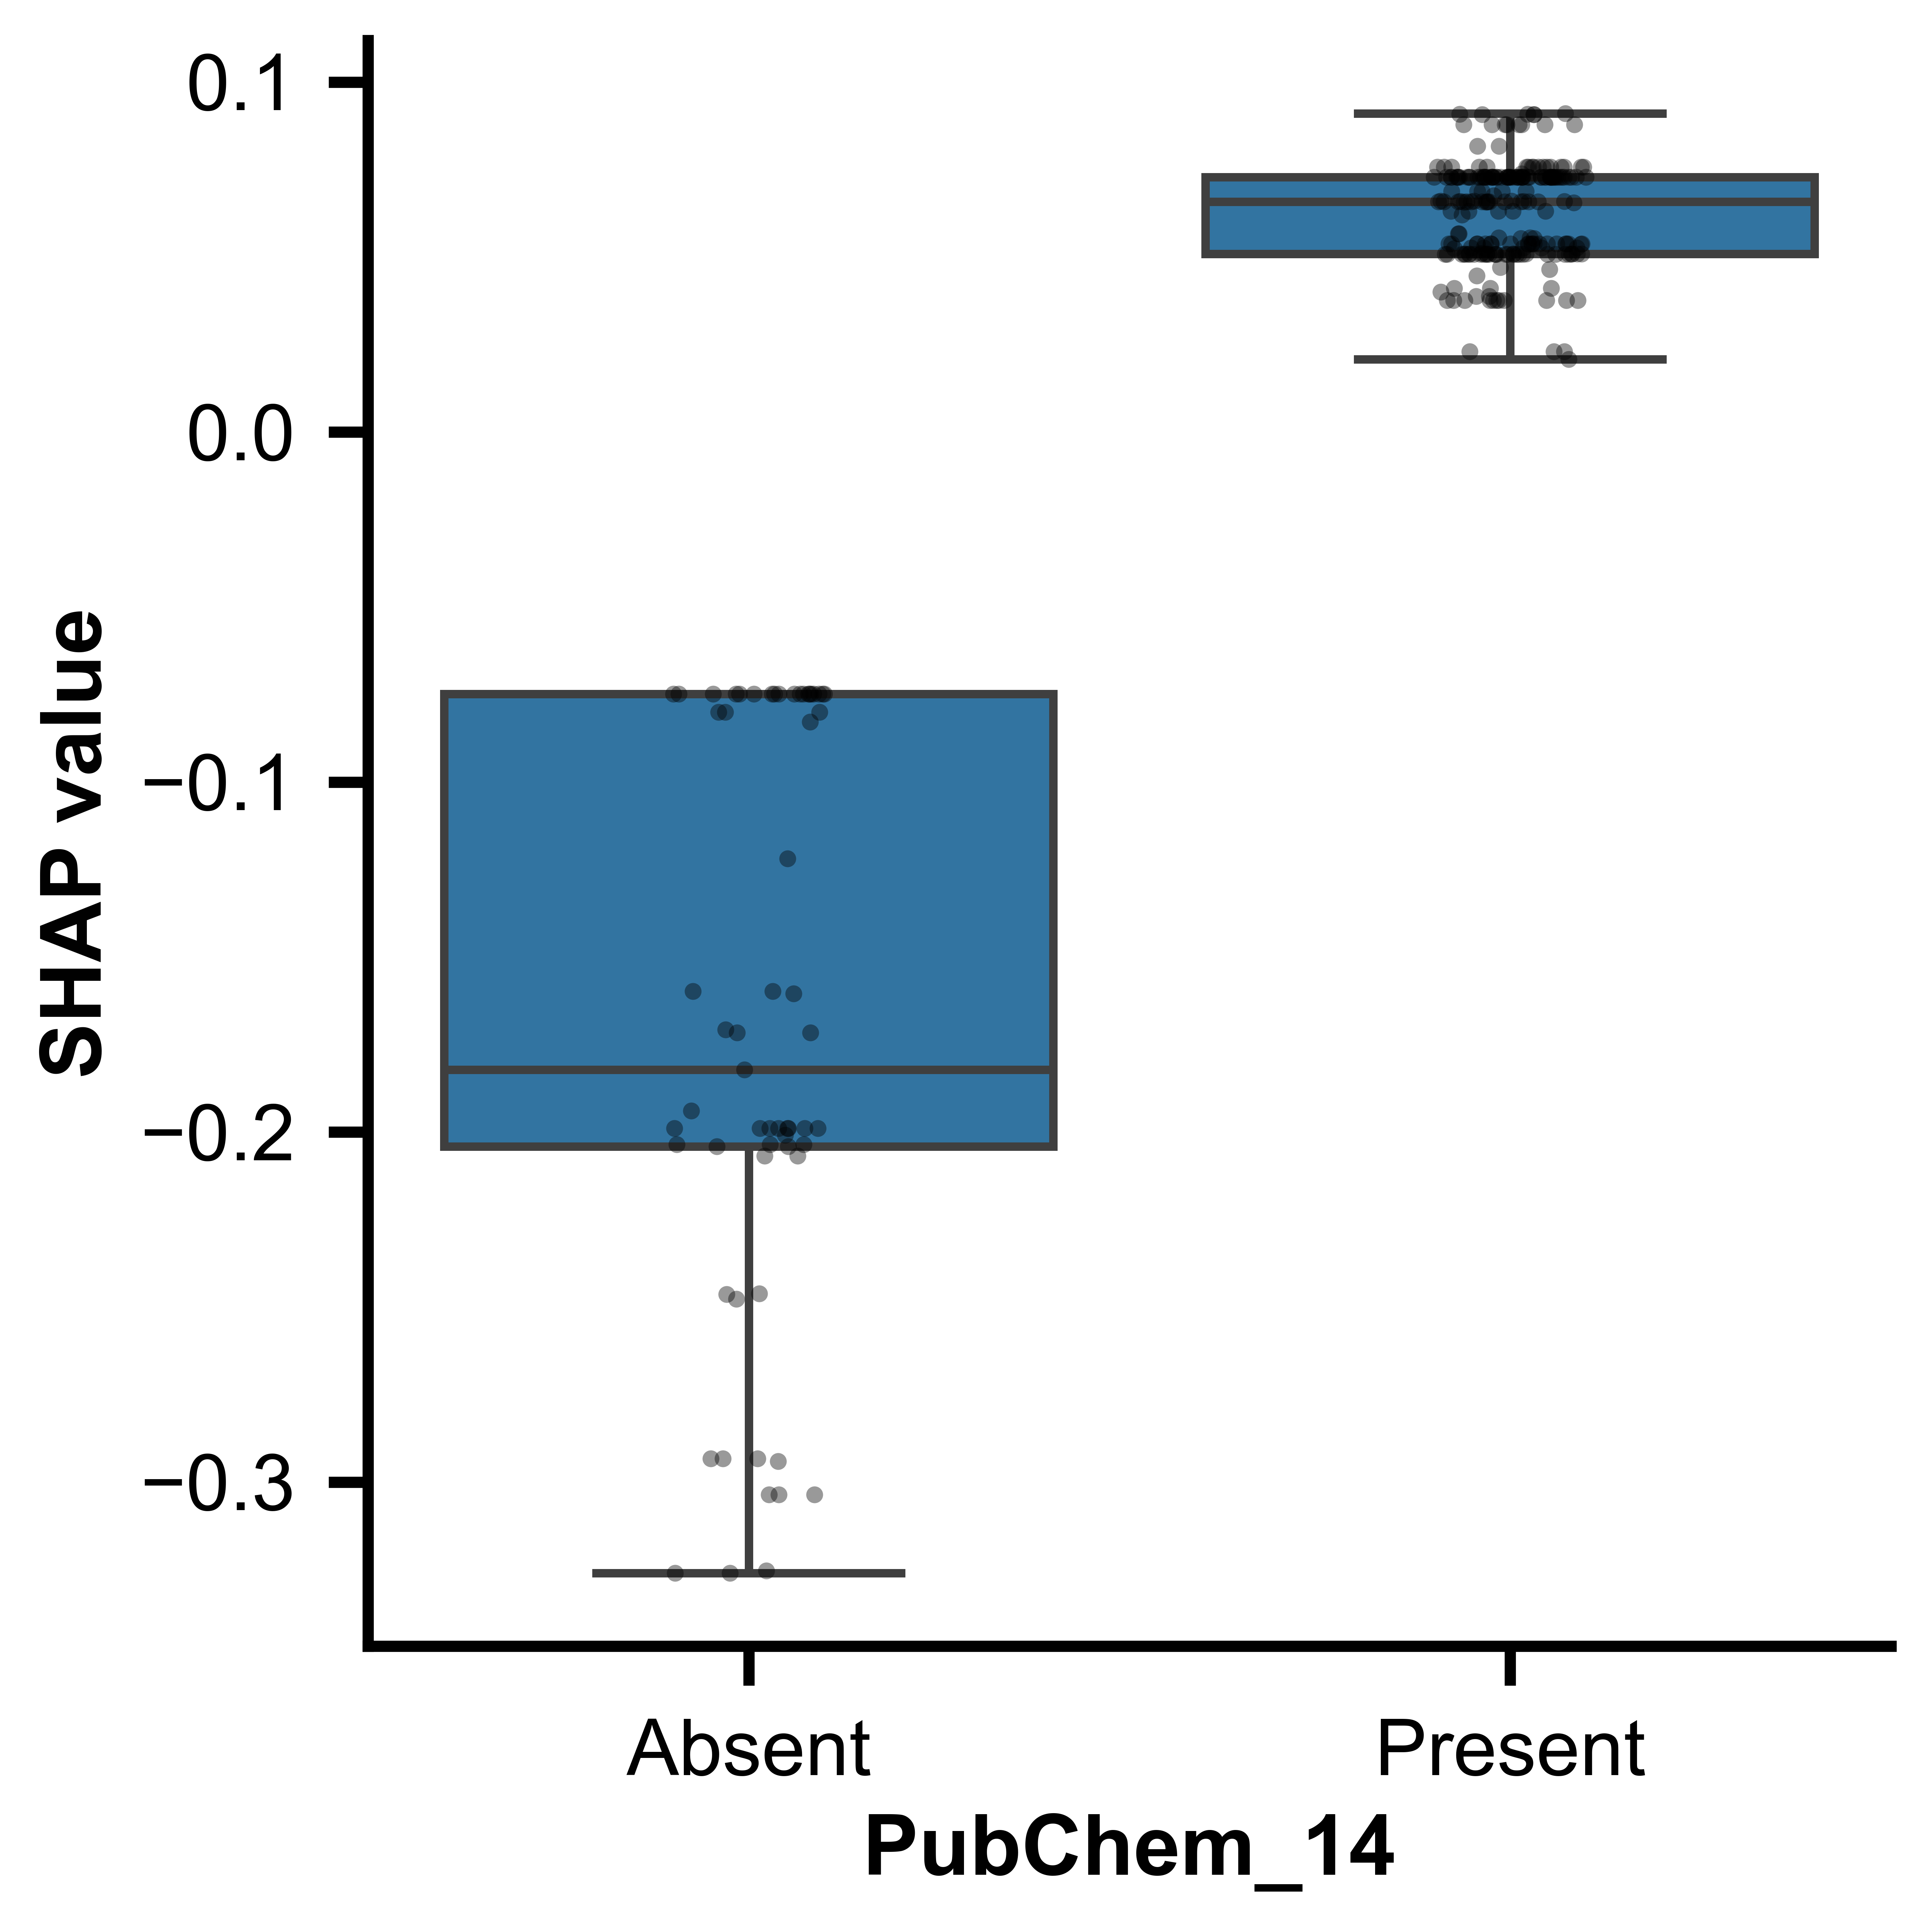
\includegraphics[width=0.37\textwidth, keepaspectratio]{prism-uploads/PubChem_14_boxplot.png} &
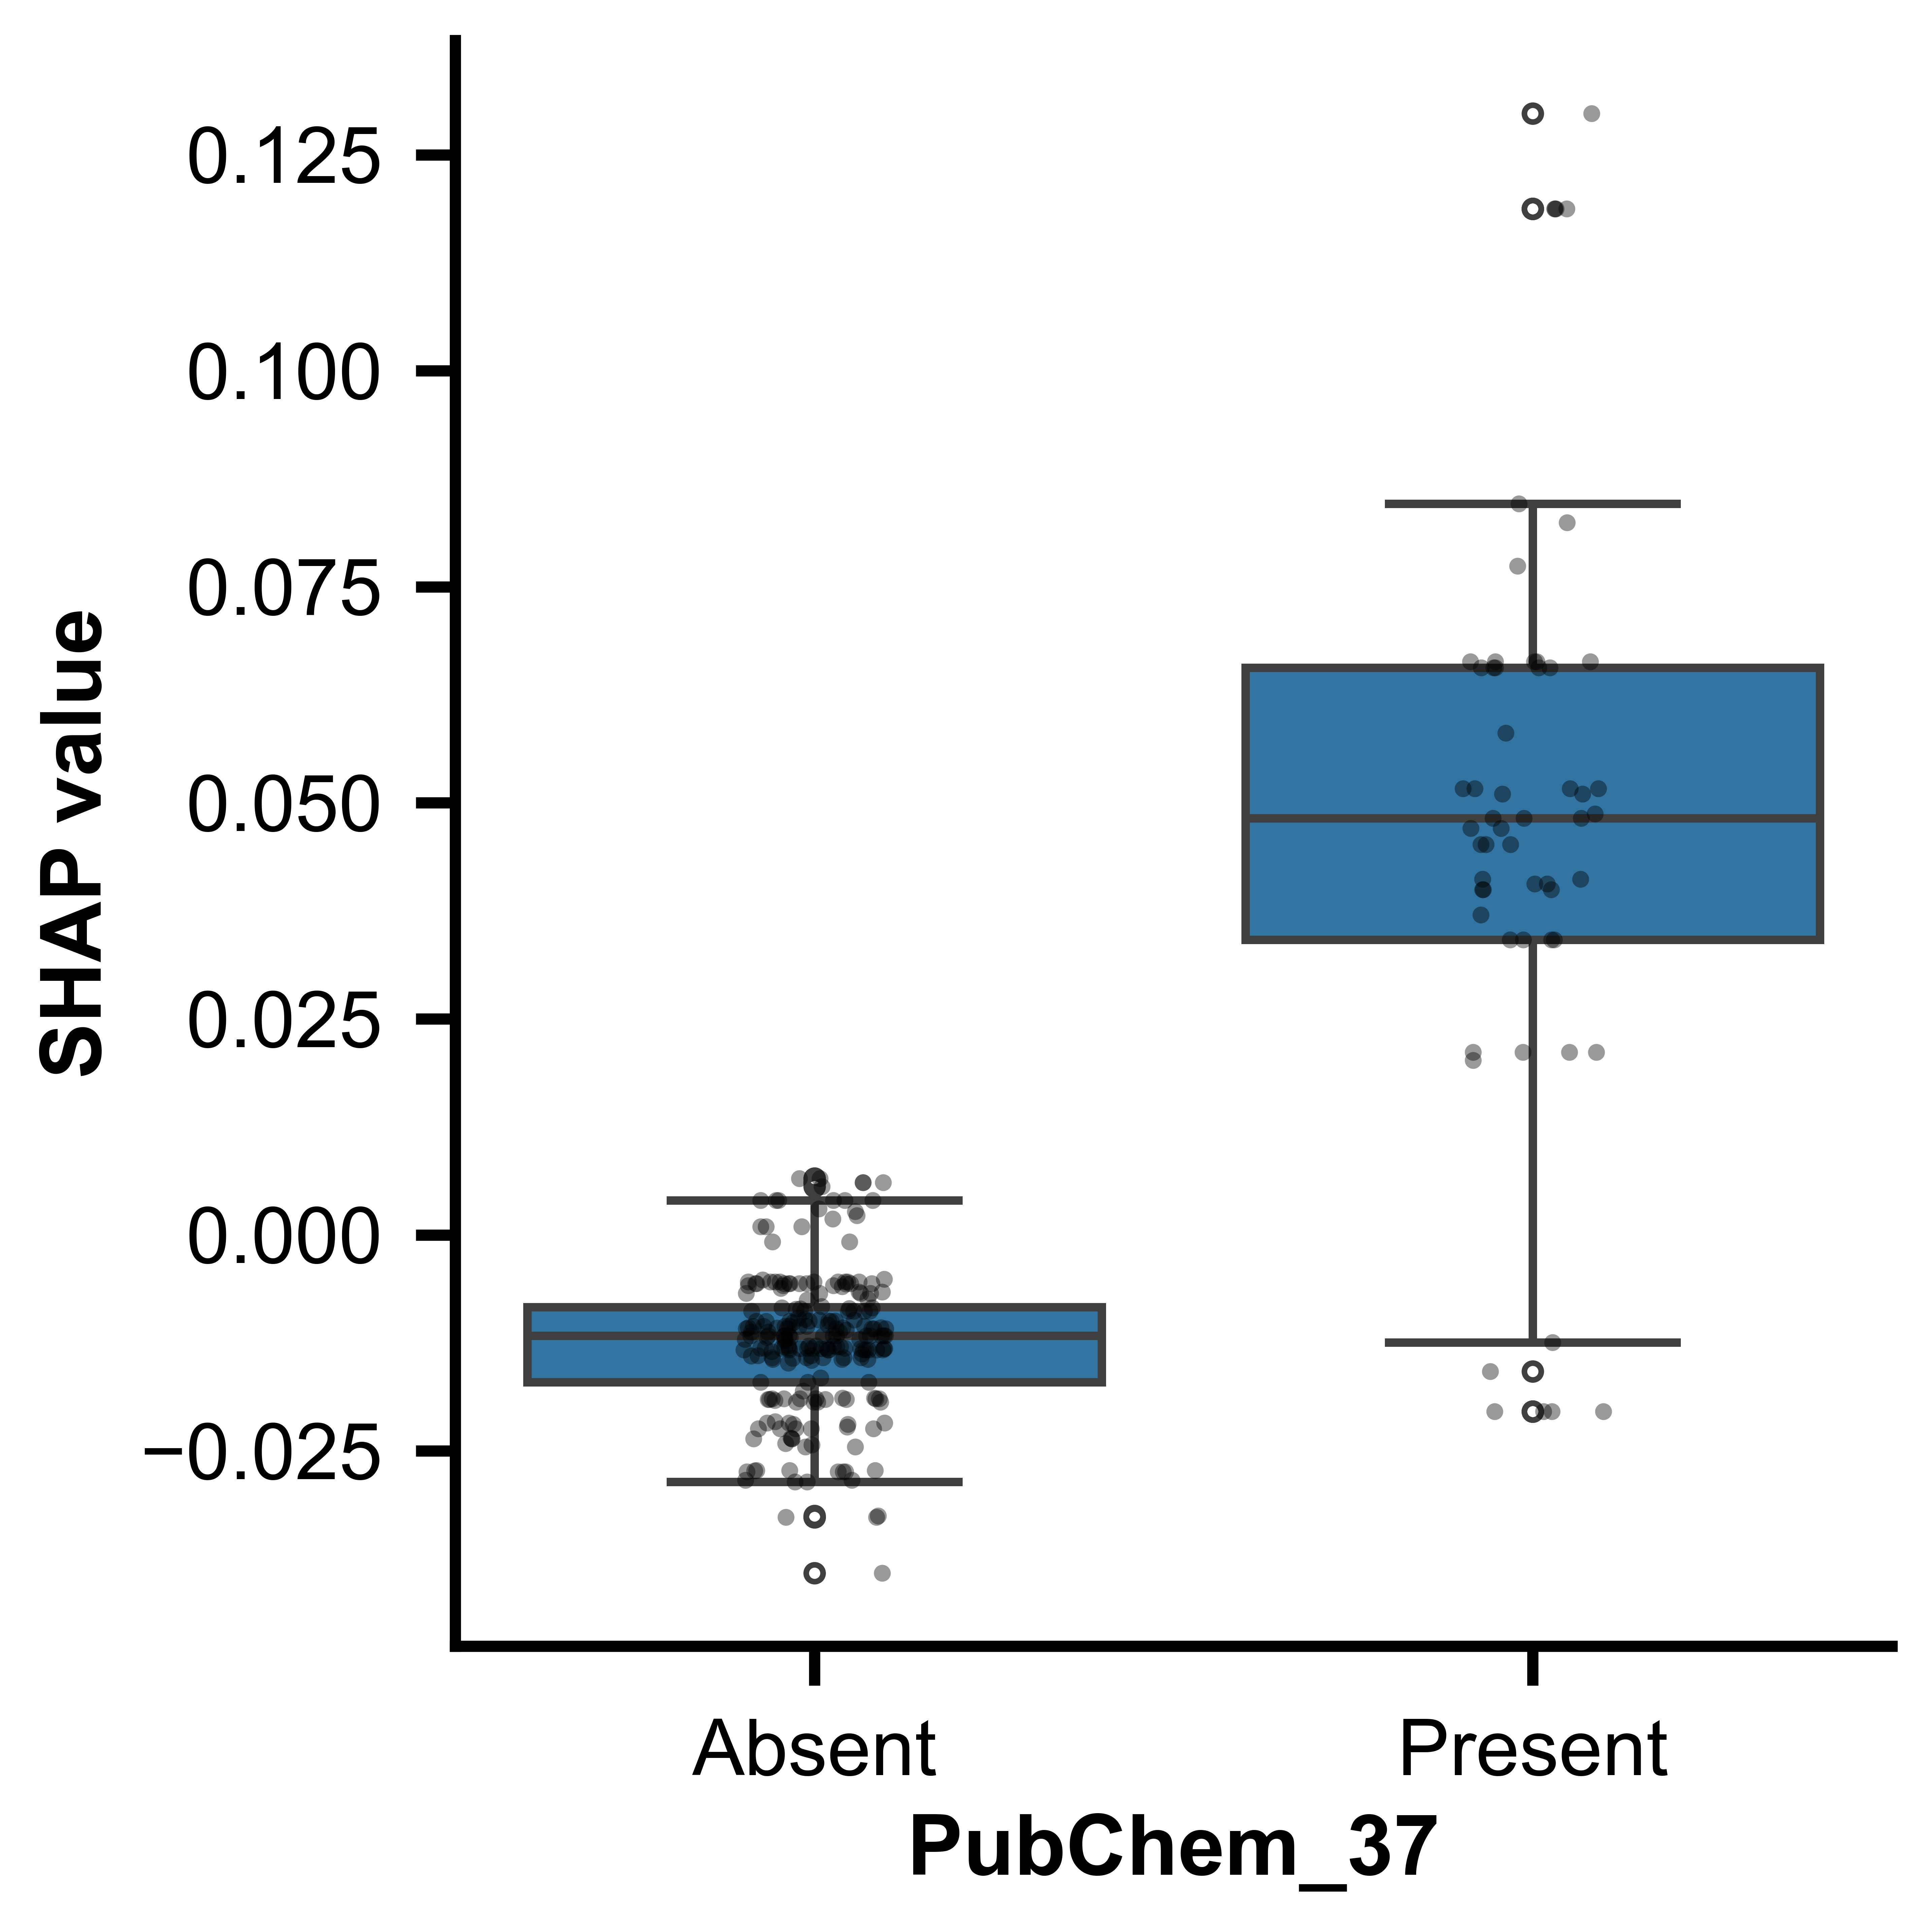
\includegraphics[width=0.37\textwidth, keepaspectratio]{prism-uploads/PubChem_37_boxplot.png} \\
(a) PubChem\_14 & (b) PubChem\_37 \\[4pt]
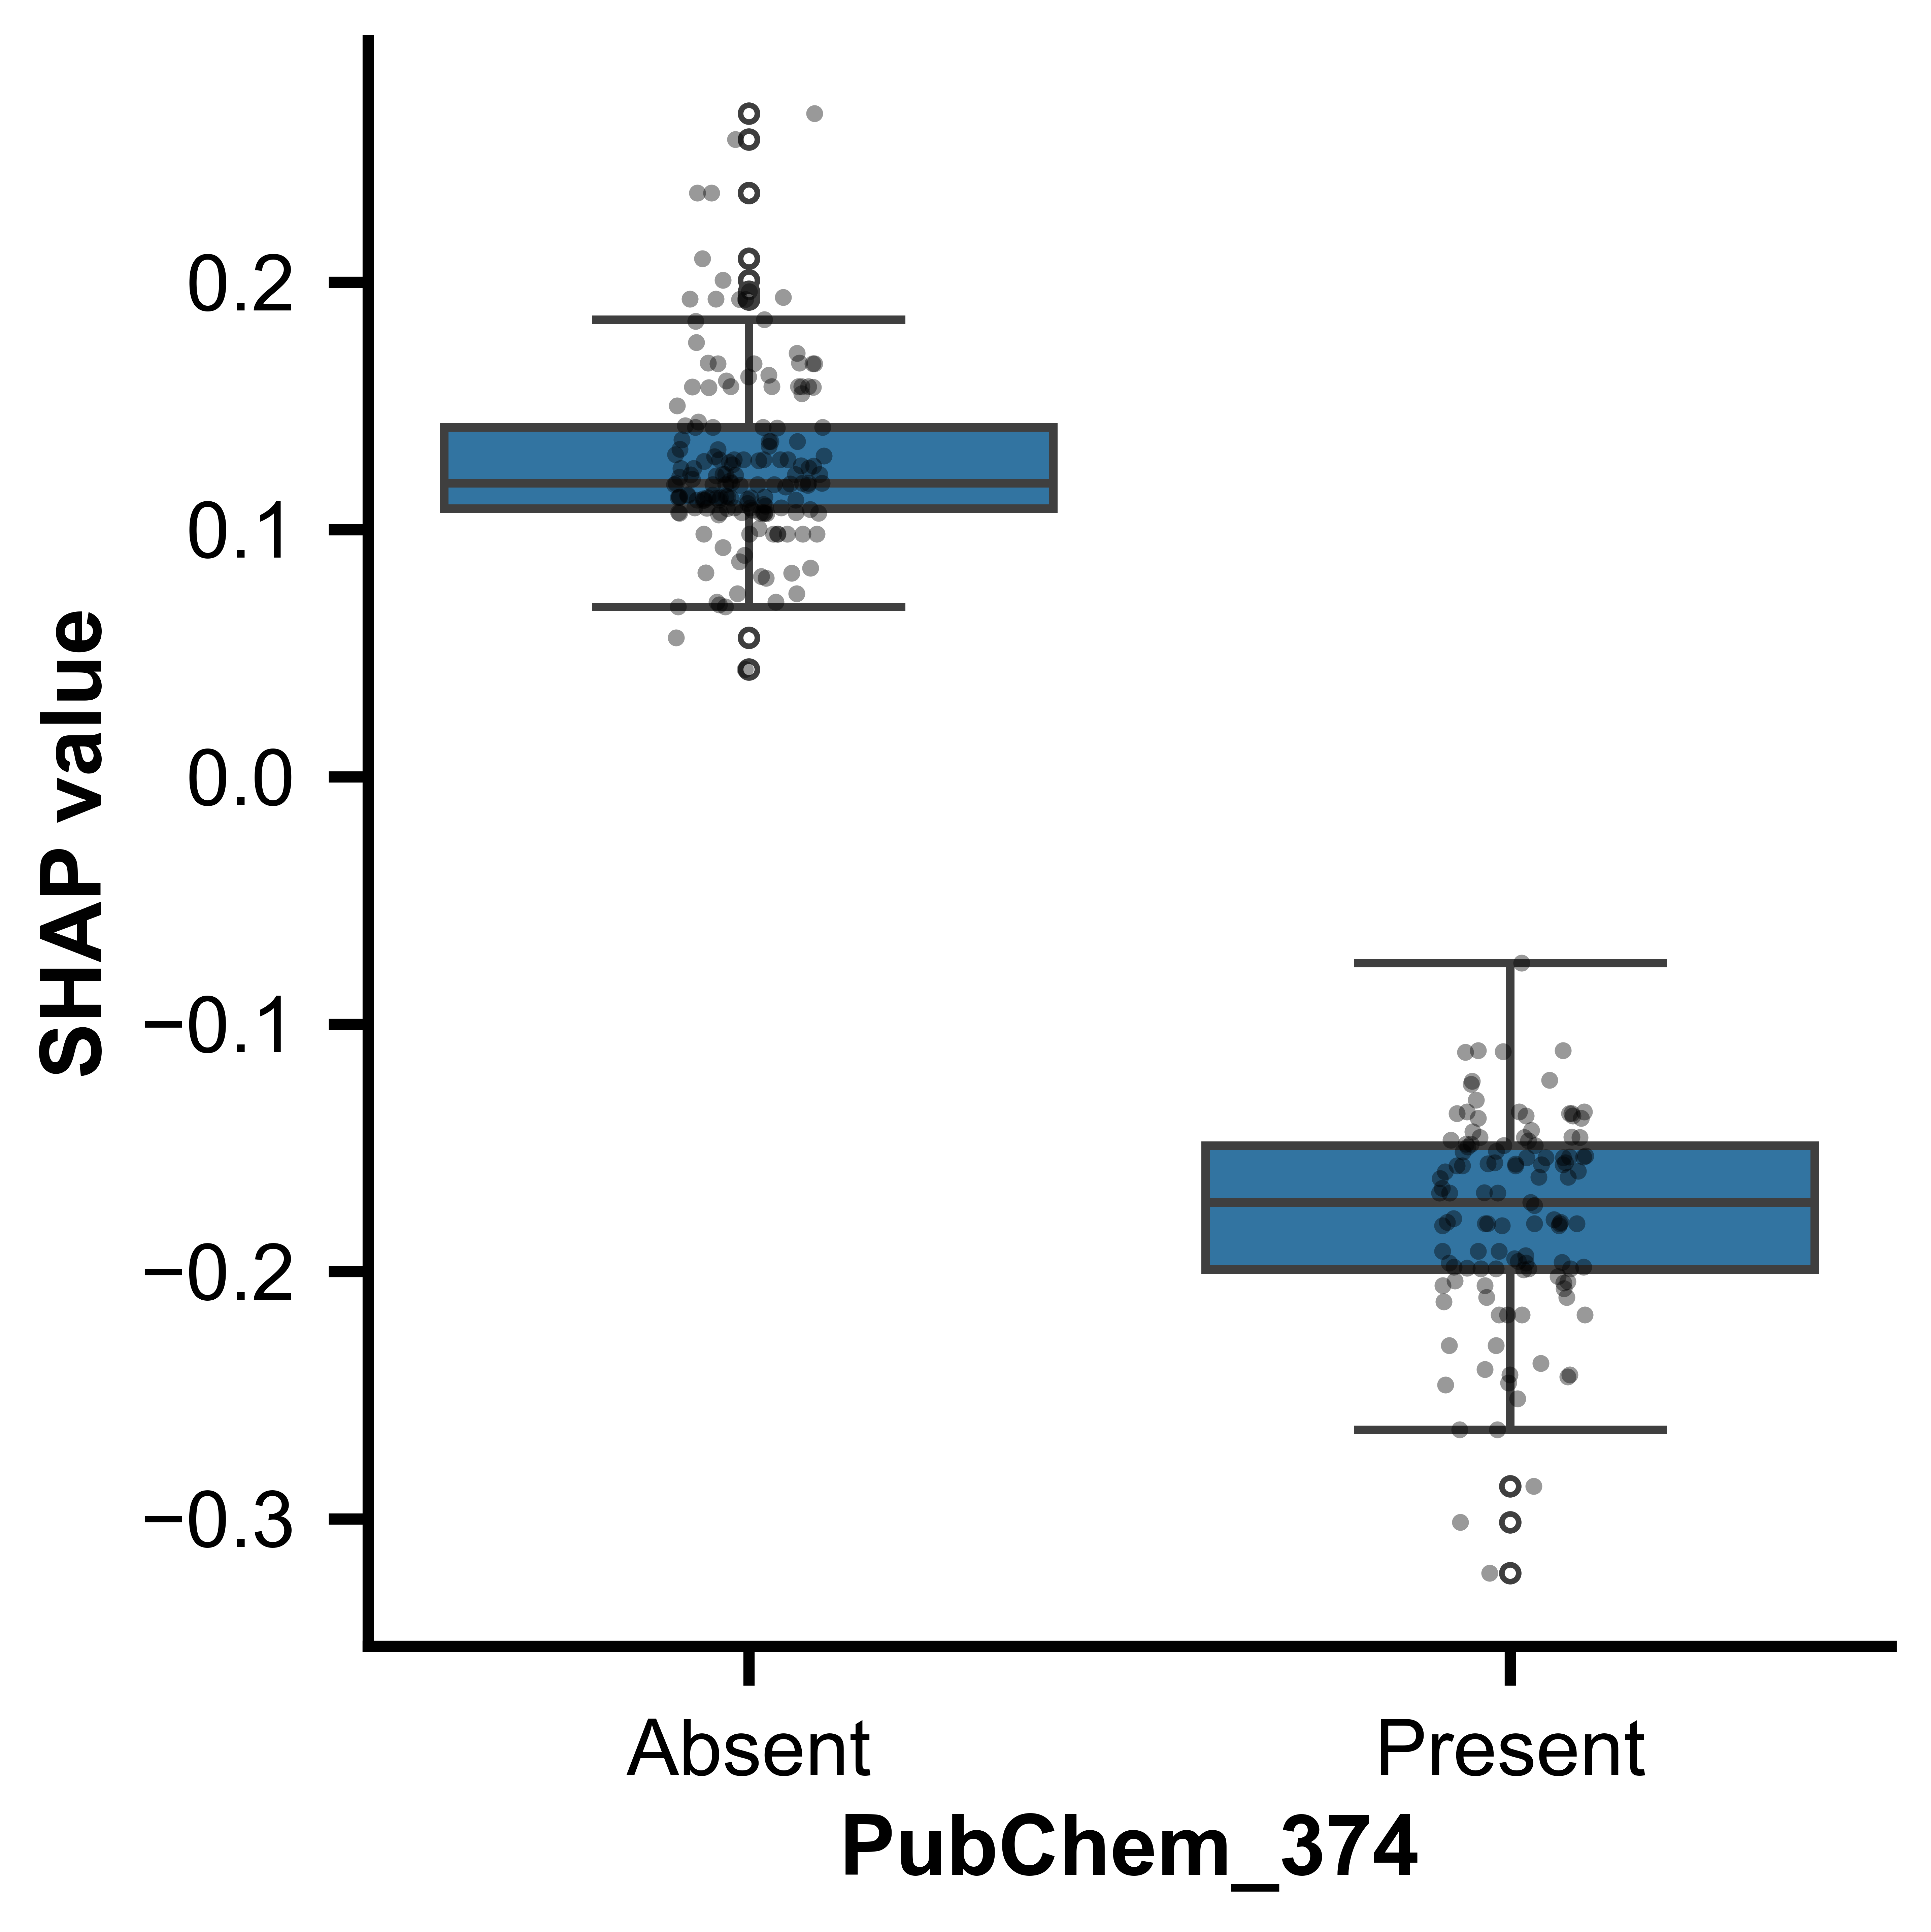
\includegraphics[width=0.37\textwidth, keepaspectratio]{prism-uploads/PubChem_374_boxplot.png} &
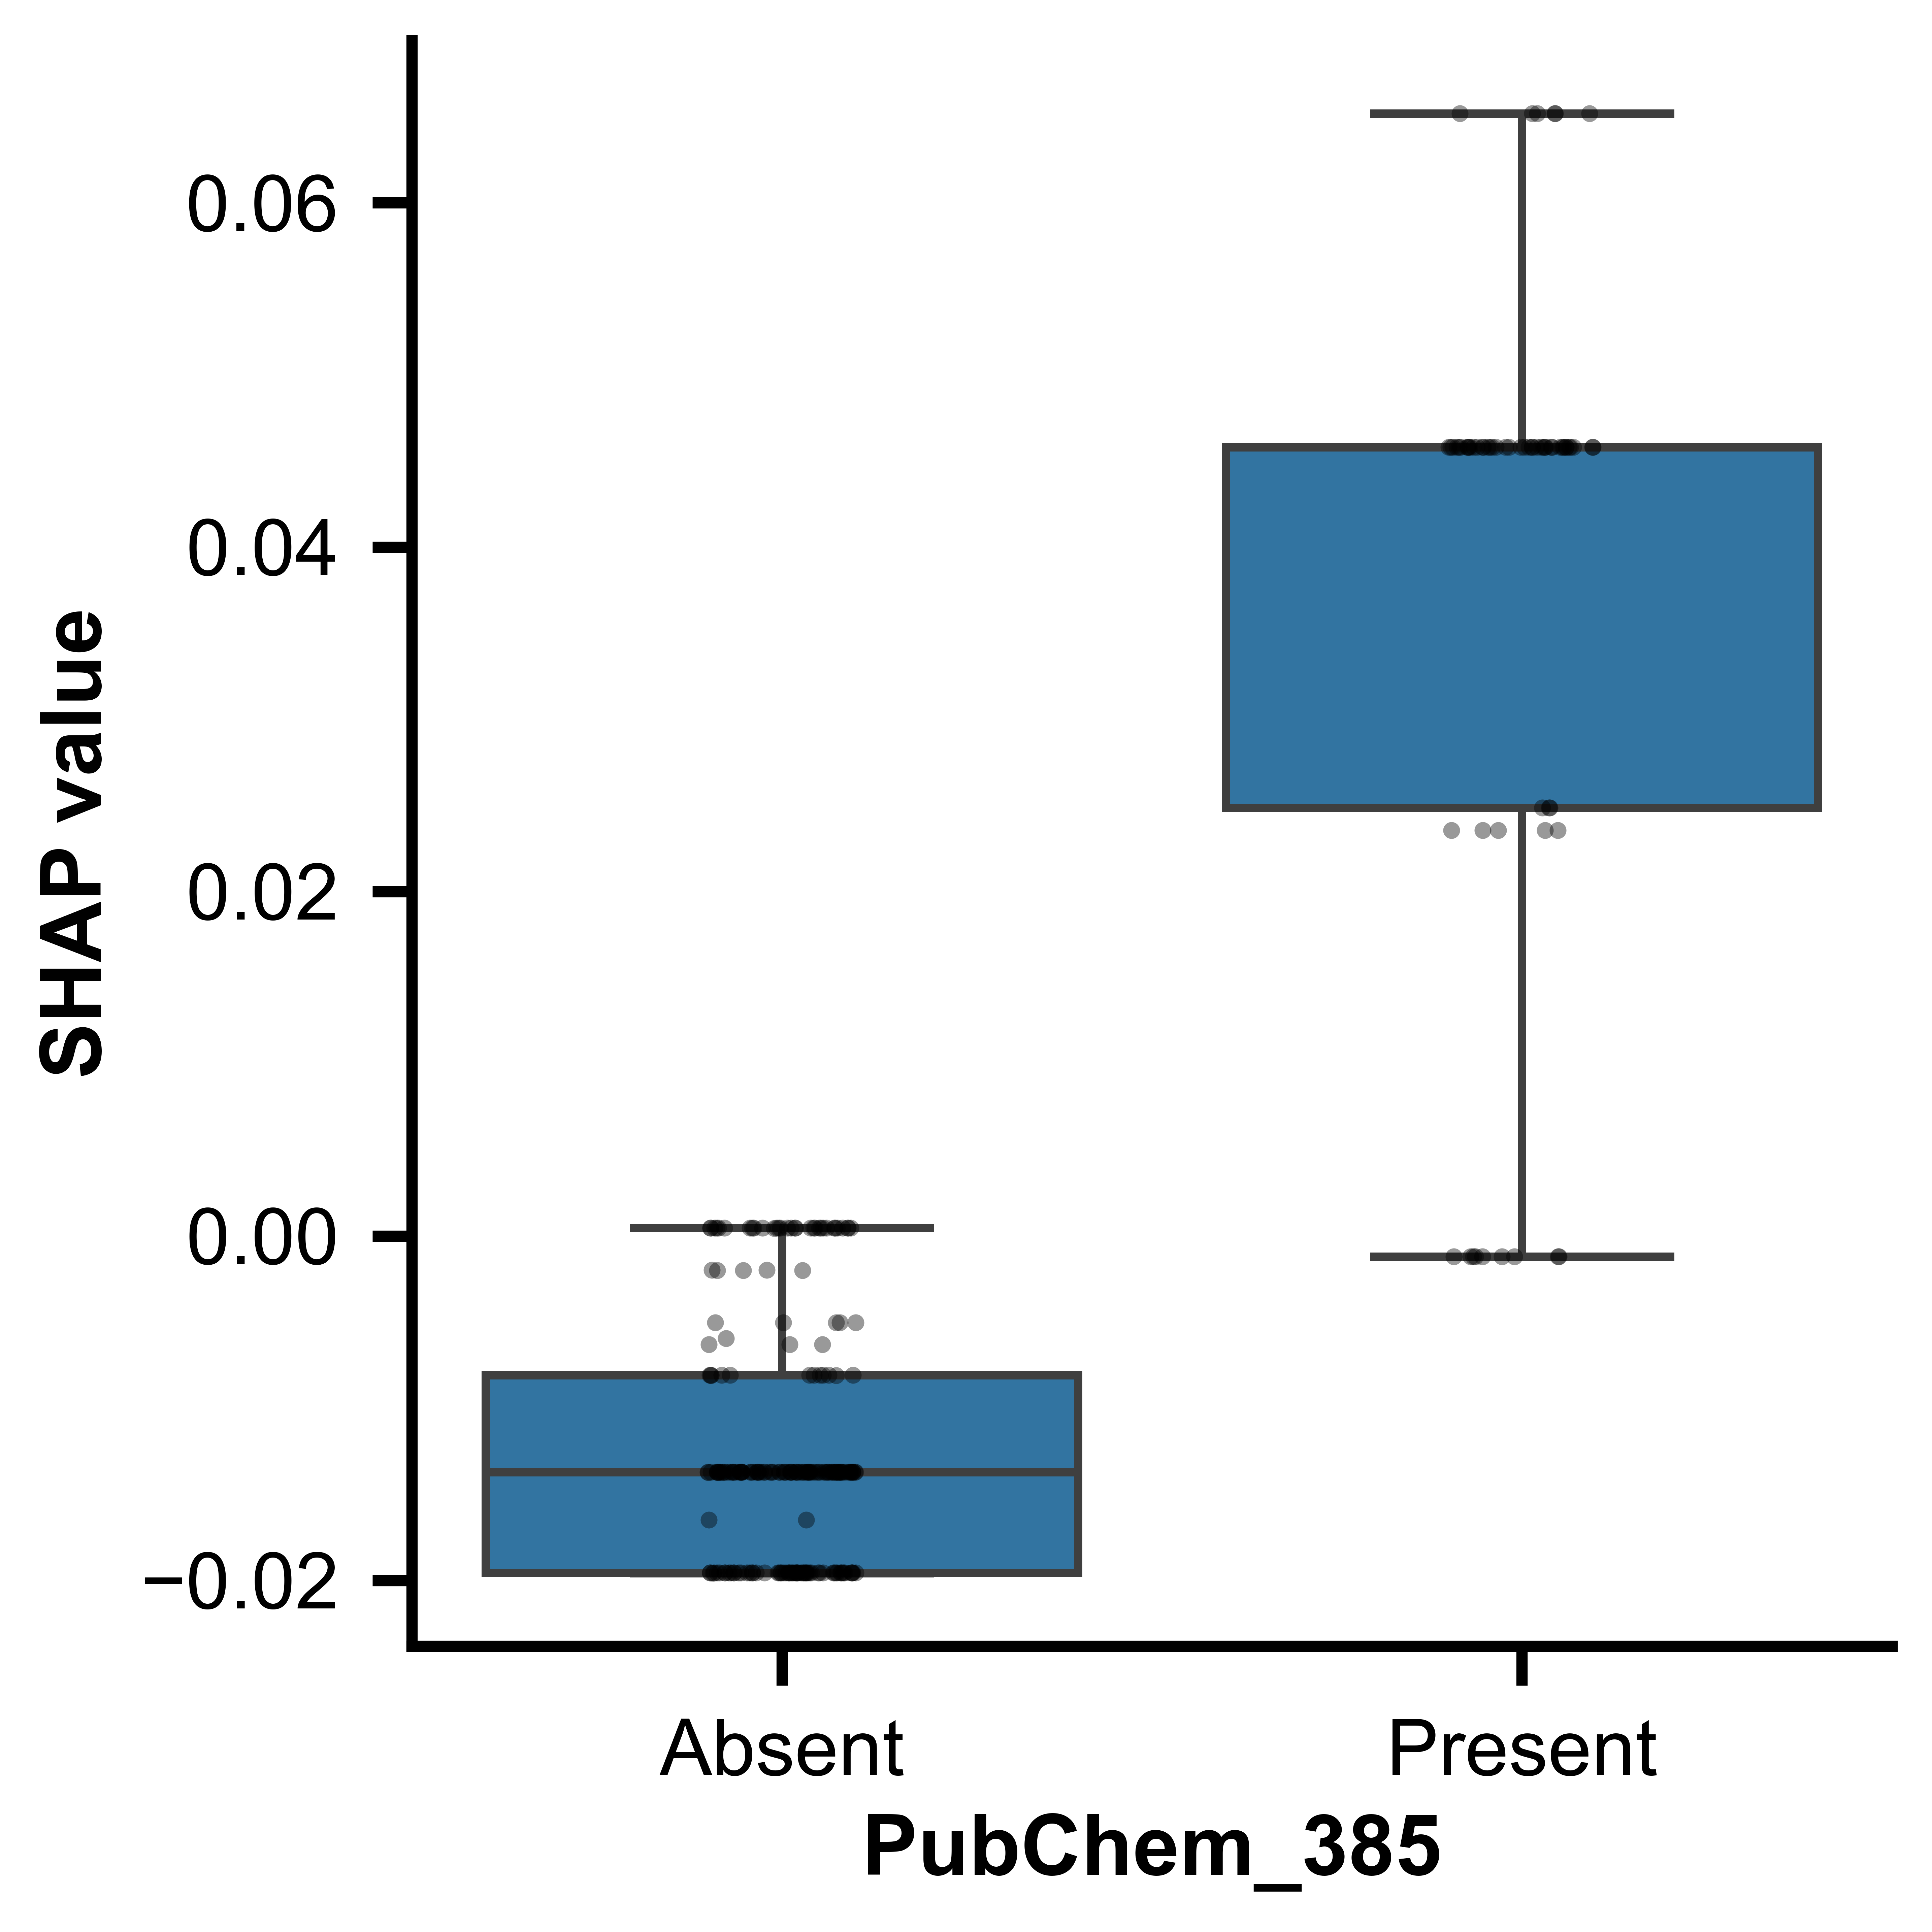
\includegraphics[width=0.37\textwidth, keepaspectratio]{prism-uploads/PubChem_385_boxplot.png} \\
(c) PubChem\_374 & (d) PubChem\_385 \\[4pt]
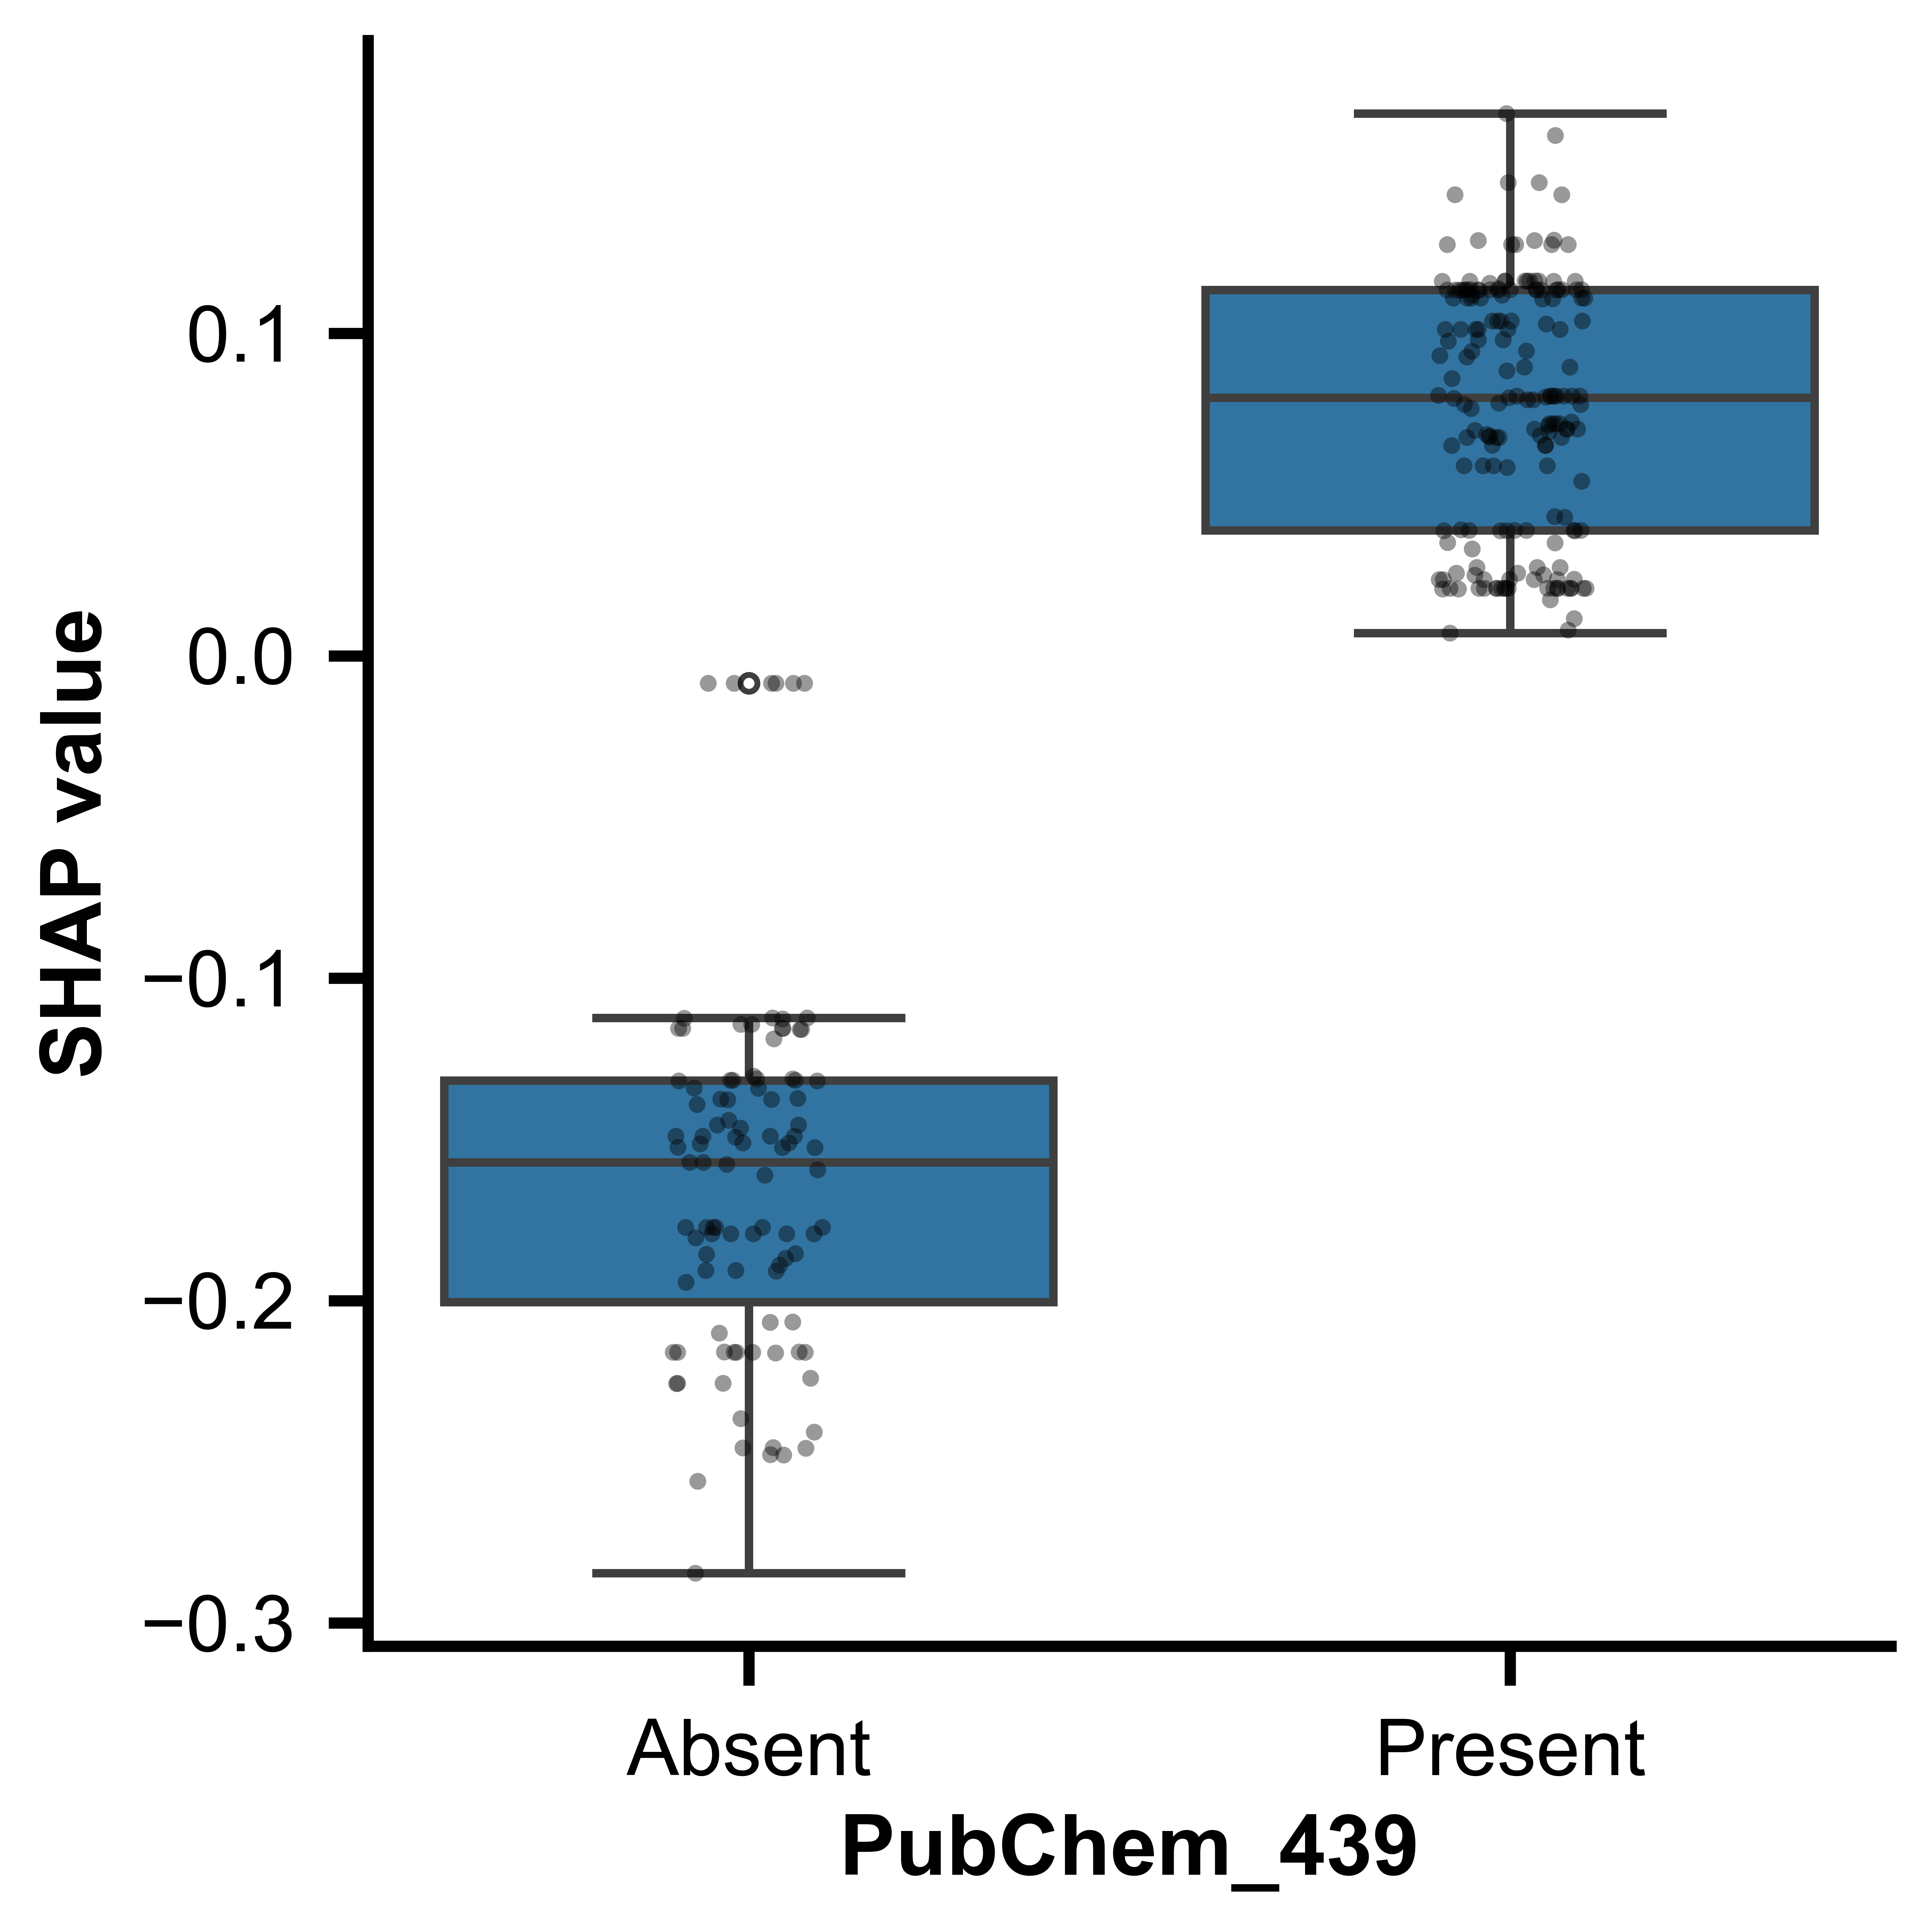
\includegraphics[width=0.37\textwidth, keepaspectratio]{prism-uploads/PubChem_439_boxplot.png} &
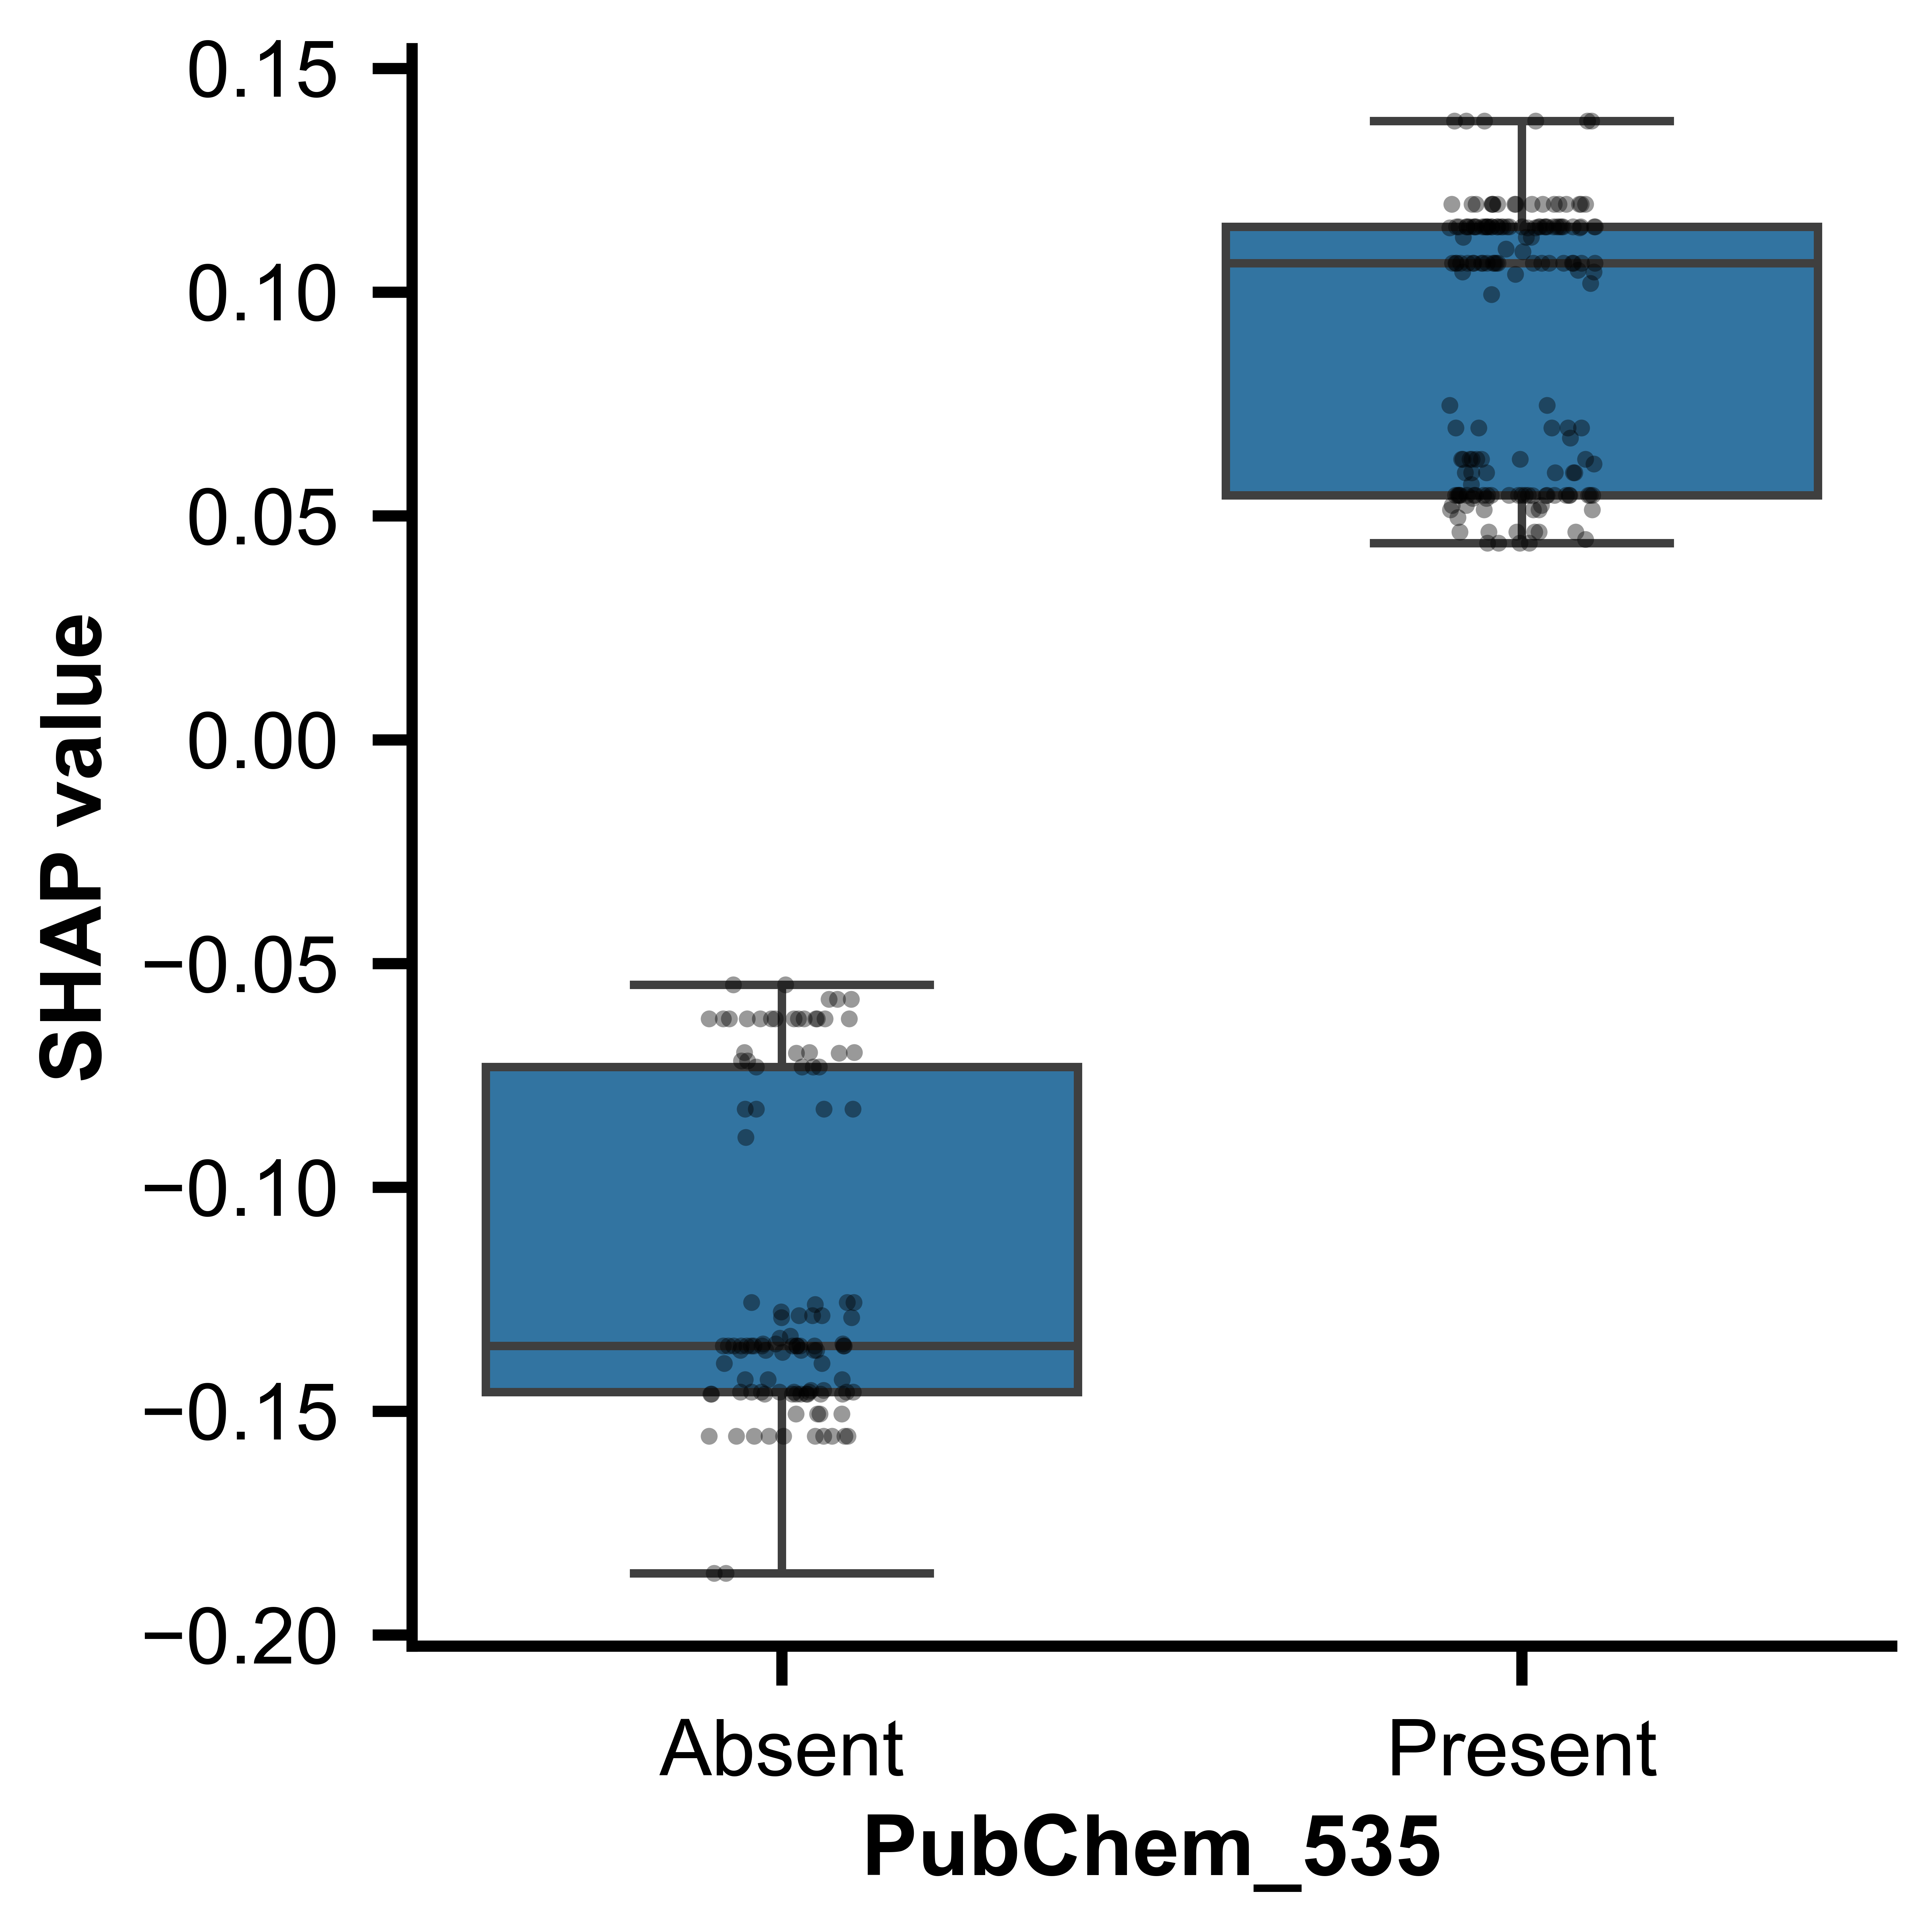
\includegraphics[width=0.37\textwidth, keepaspectratio]{prism-uploads/PubChem_535_boxplot.png} \\
(e) PubChem\_439 & (f) PubChem\_535 \\
\end{tabular}
\caption[Boxplot distributions for SHAP-ranked PubChem descriptors, part 1]{Boxplot distributions of pIC$_{50}$ values grouped by the absence or presence of selected SHAP-ranked PubChem fingerprint descriptors. Panels show PubChem\_14, PubChem\_37, PubChem\_374, PubChem\_385, PubChem\_439, and PubChem\_535.}
\label{fig:pubchem-boxplots-1}
\end{figure}

\begin{figure}[p]
\centering
\scriptsize
\begin{tabular}{cc}
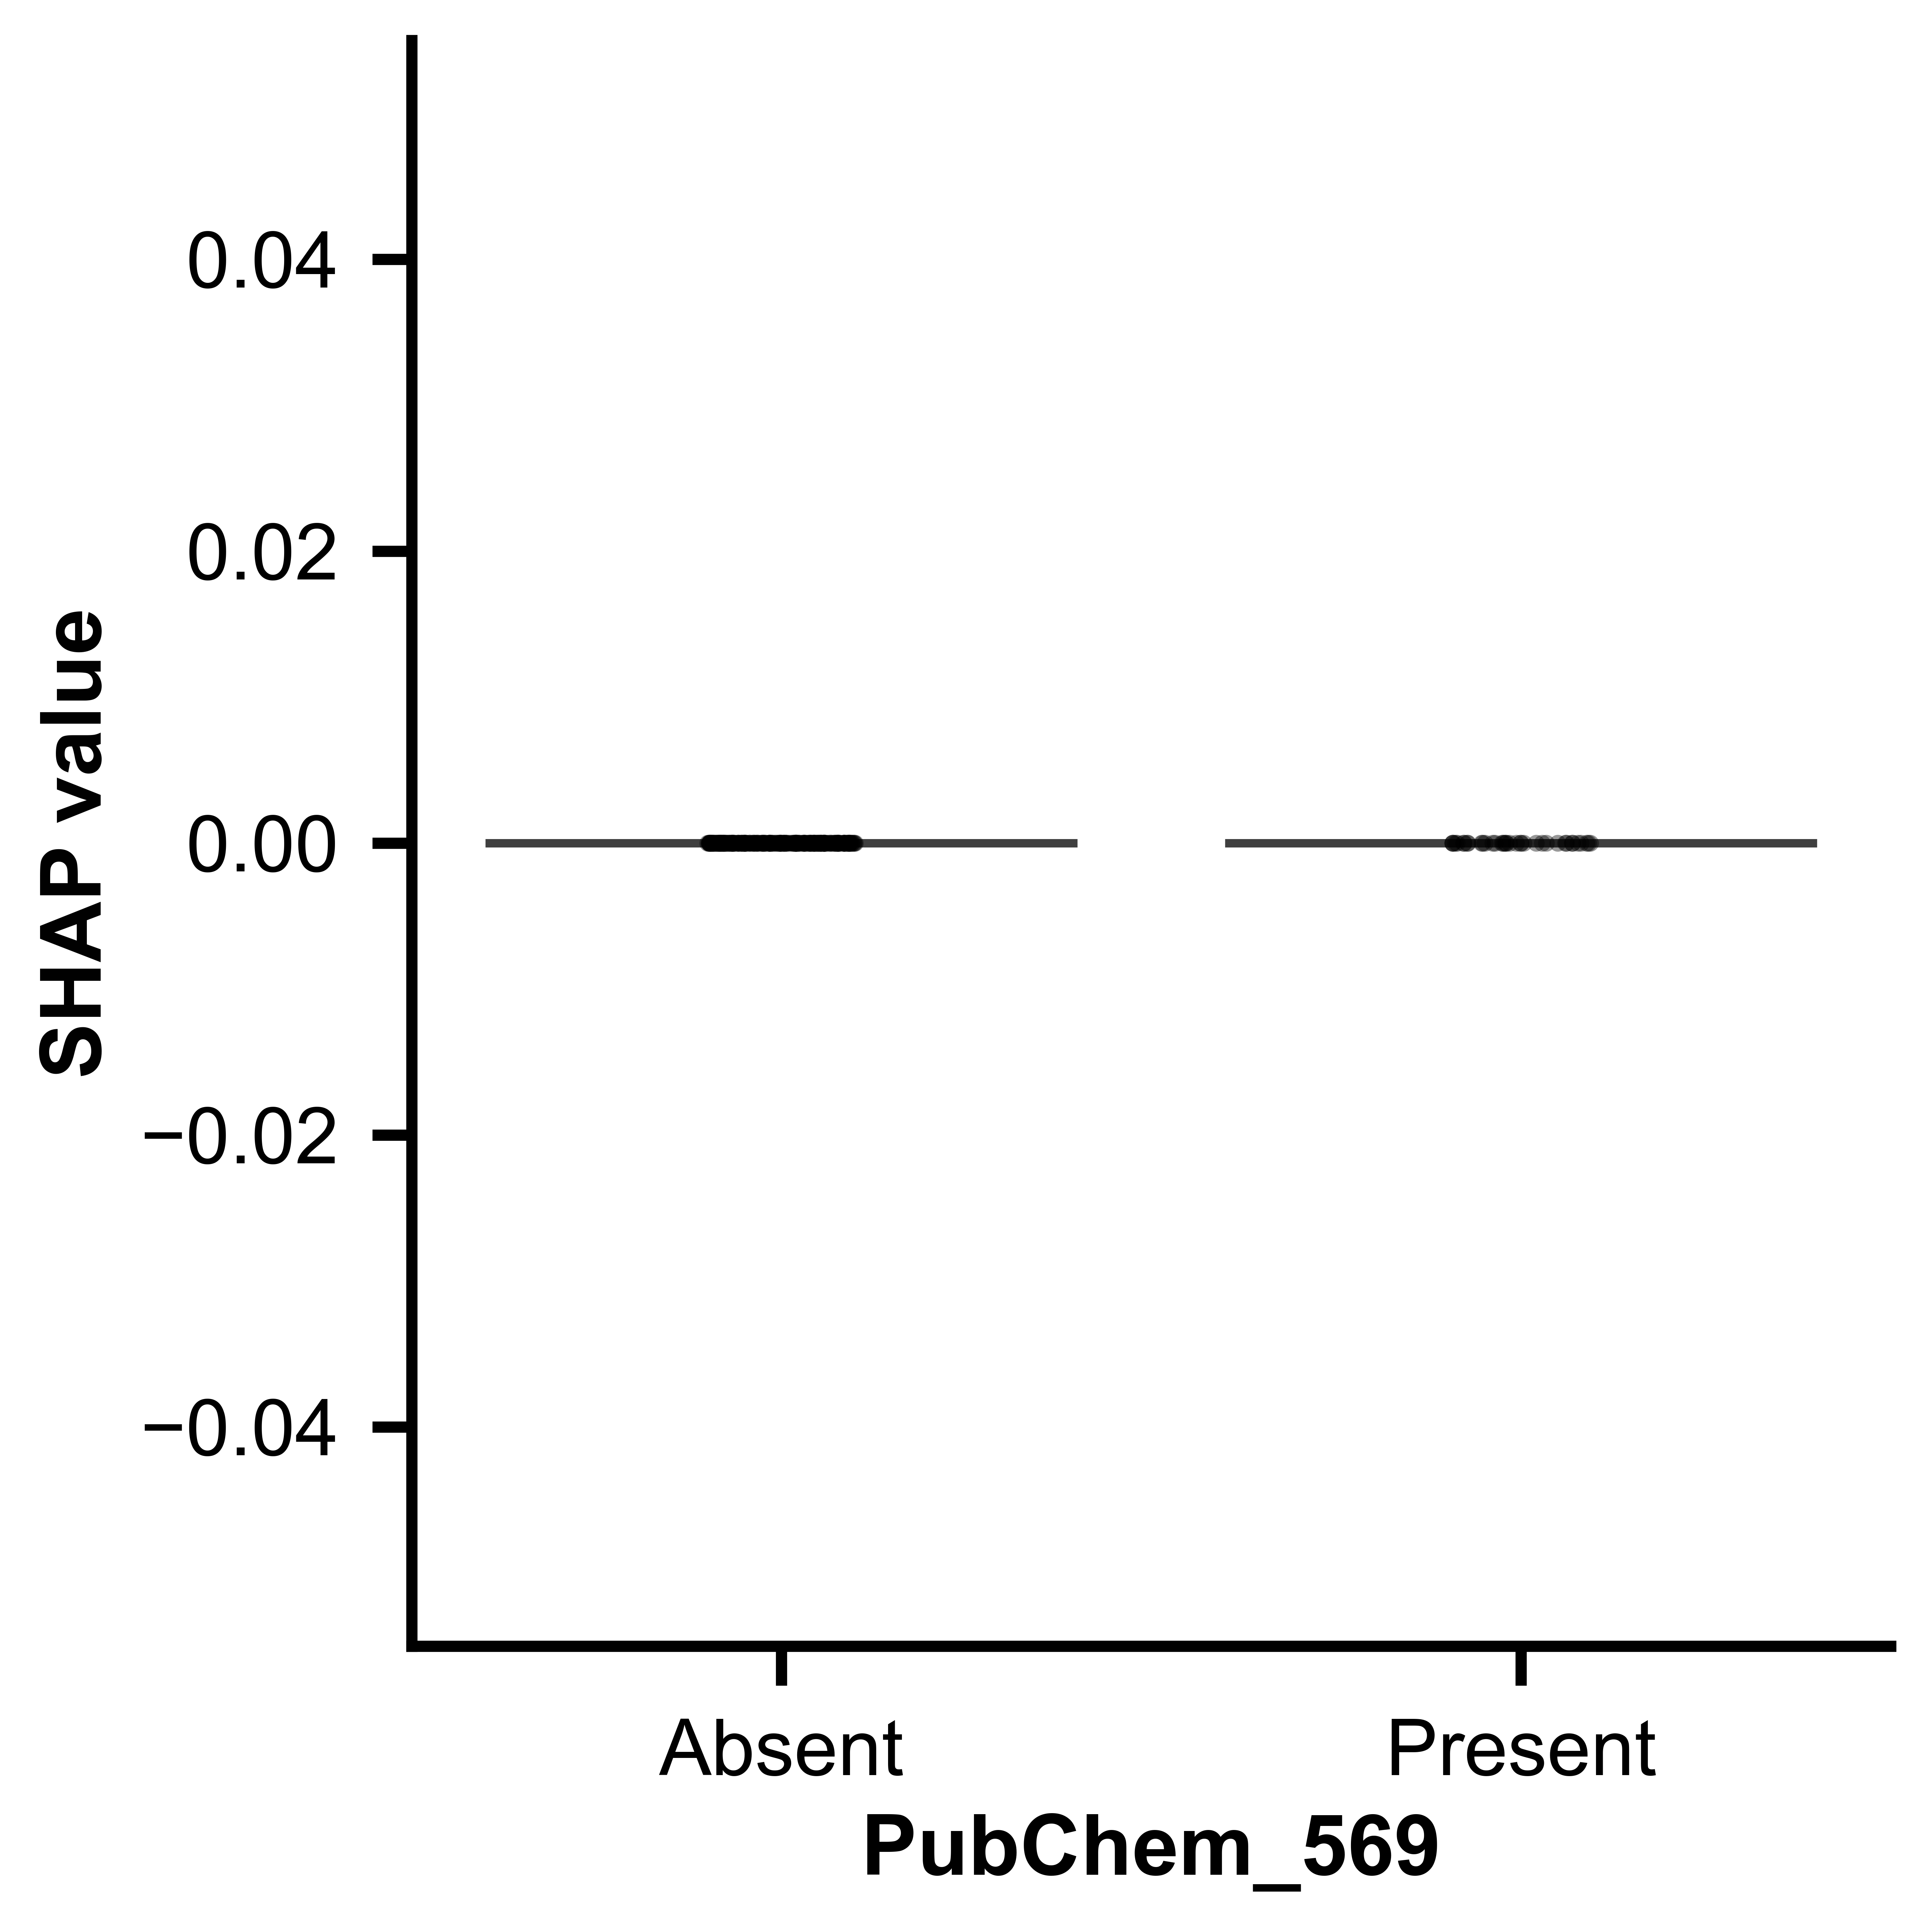
\includegraphics[width=0.43\textwidth, keepaspectratio]{prism-uploads/PubChem_569_boxplot.png} &
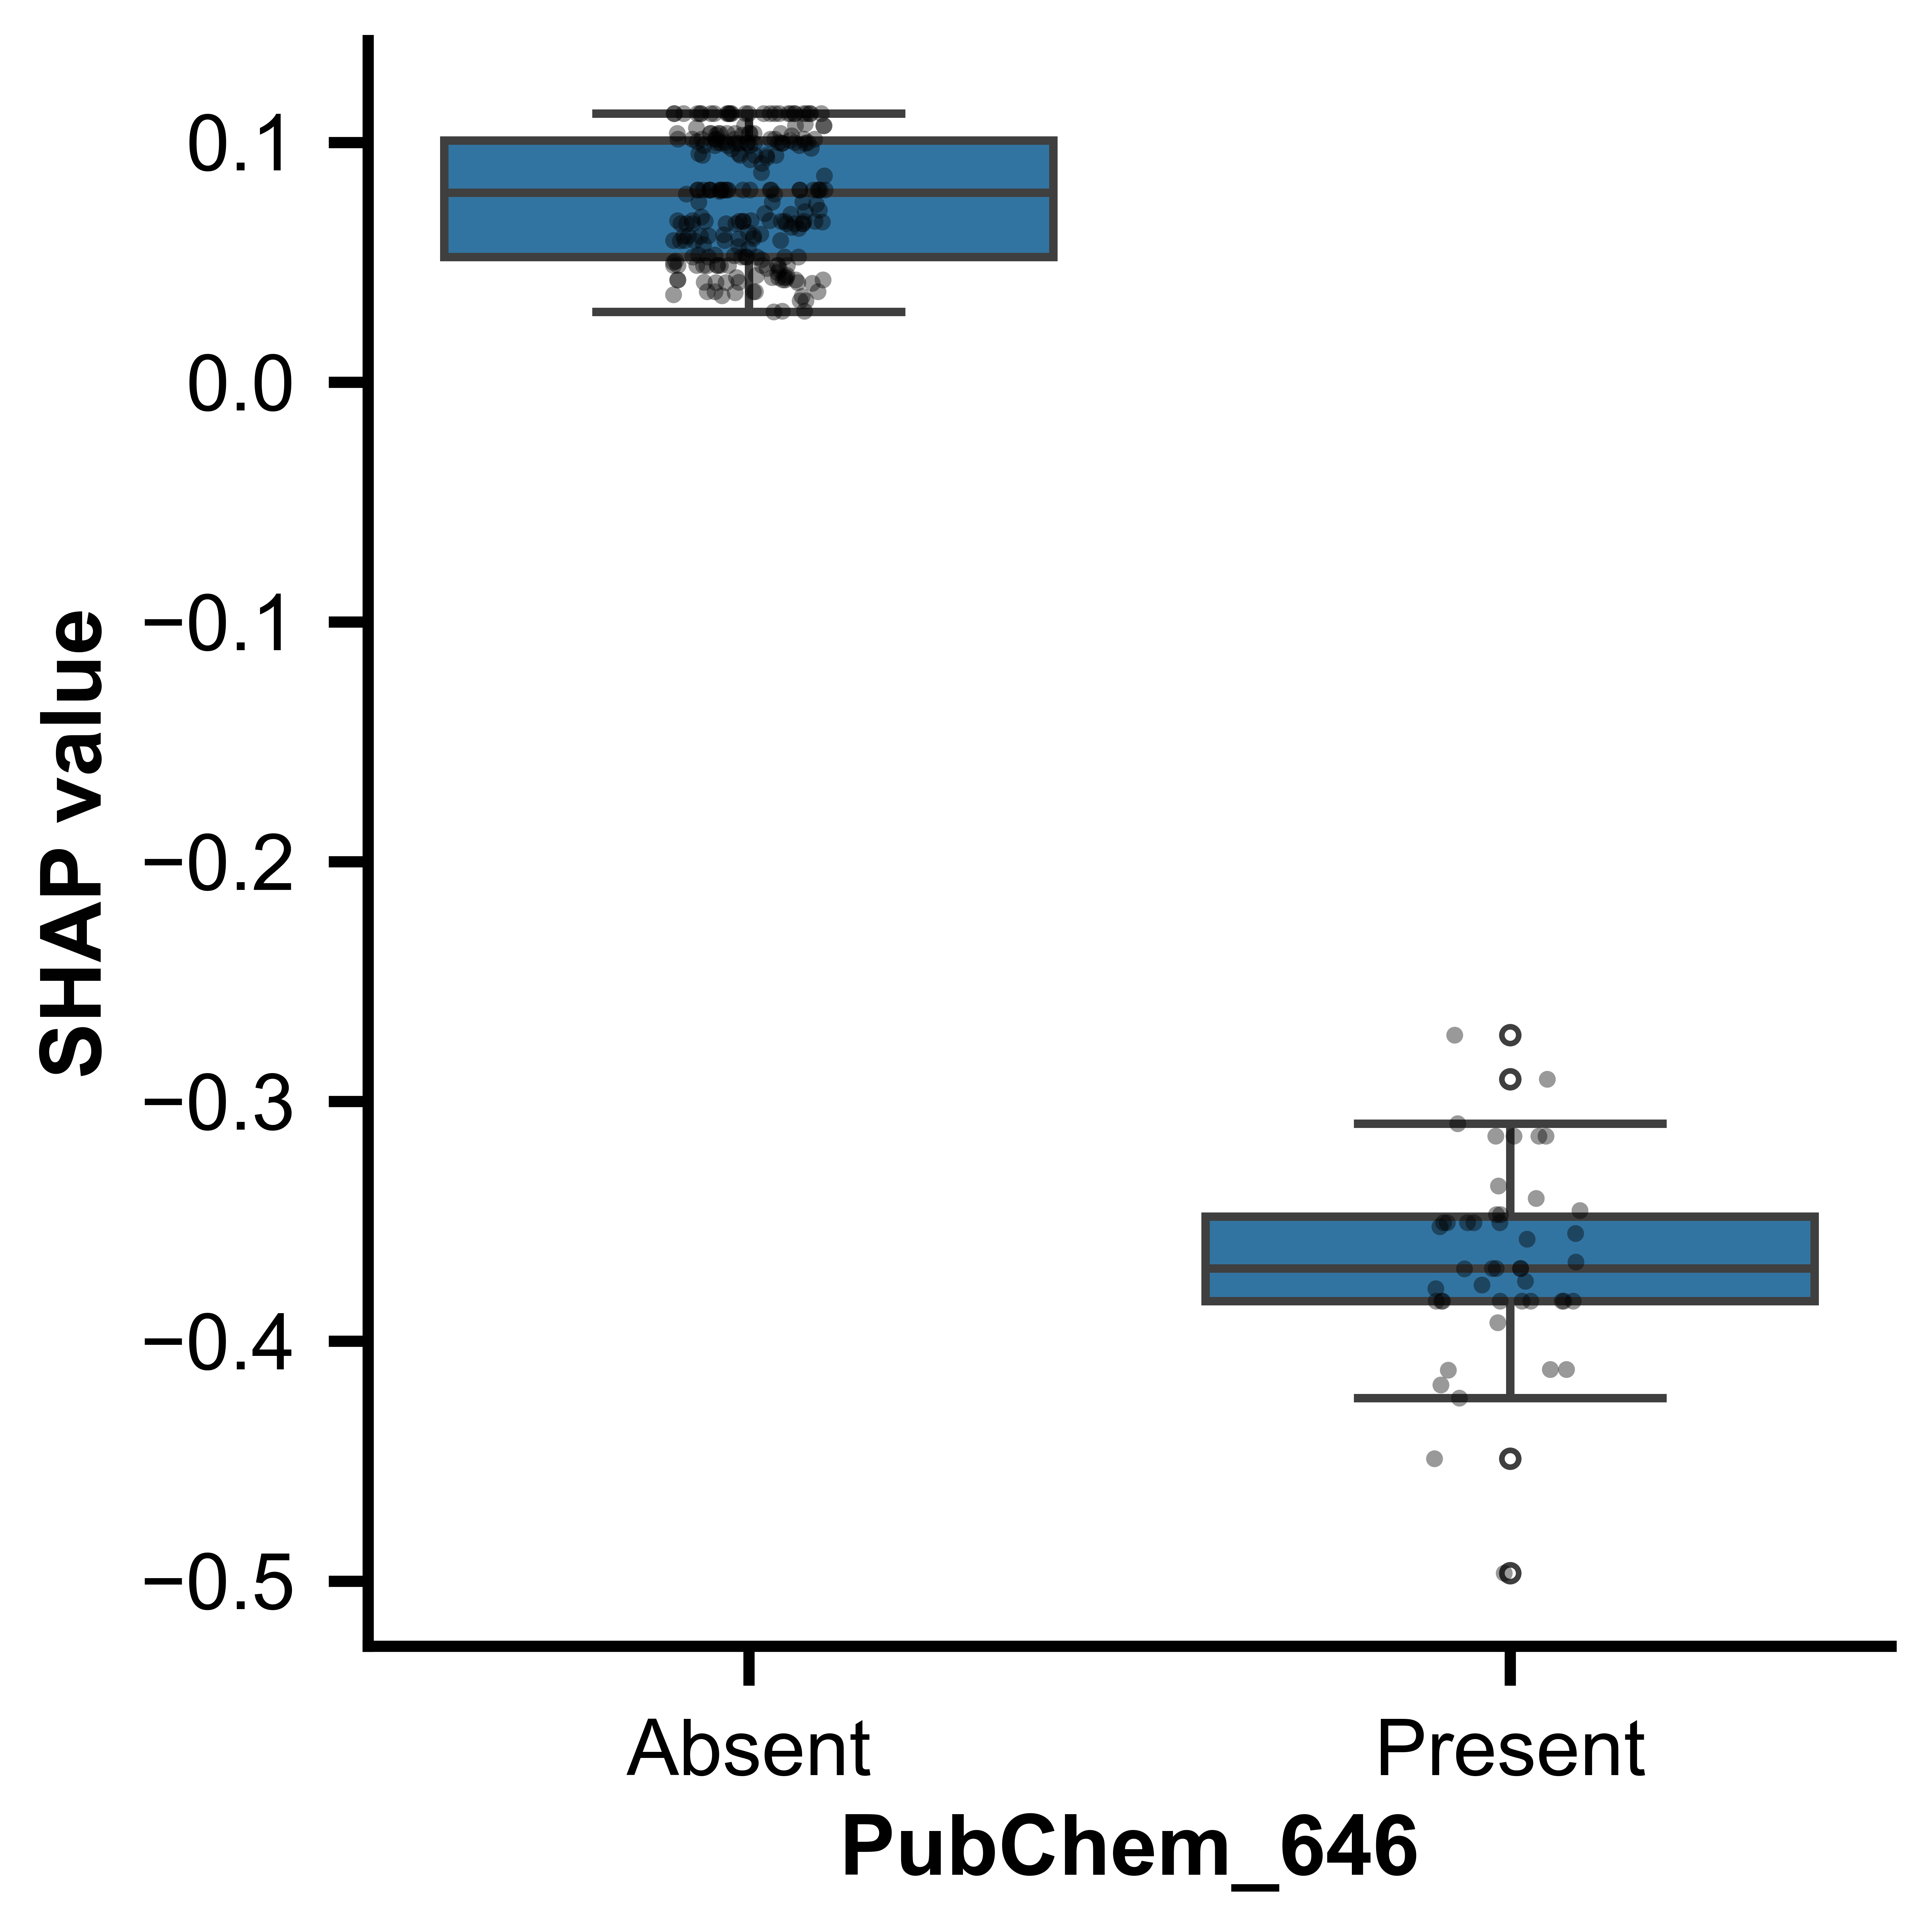
\includegraphics[width=0.43\textwidth, keepaspectratio]{prism-uploads/PubChem_646_boxplot.png} \\
(a) PubChem\_569 & (b) PubChem\_646 \\[4pt]
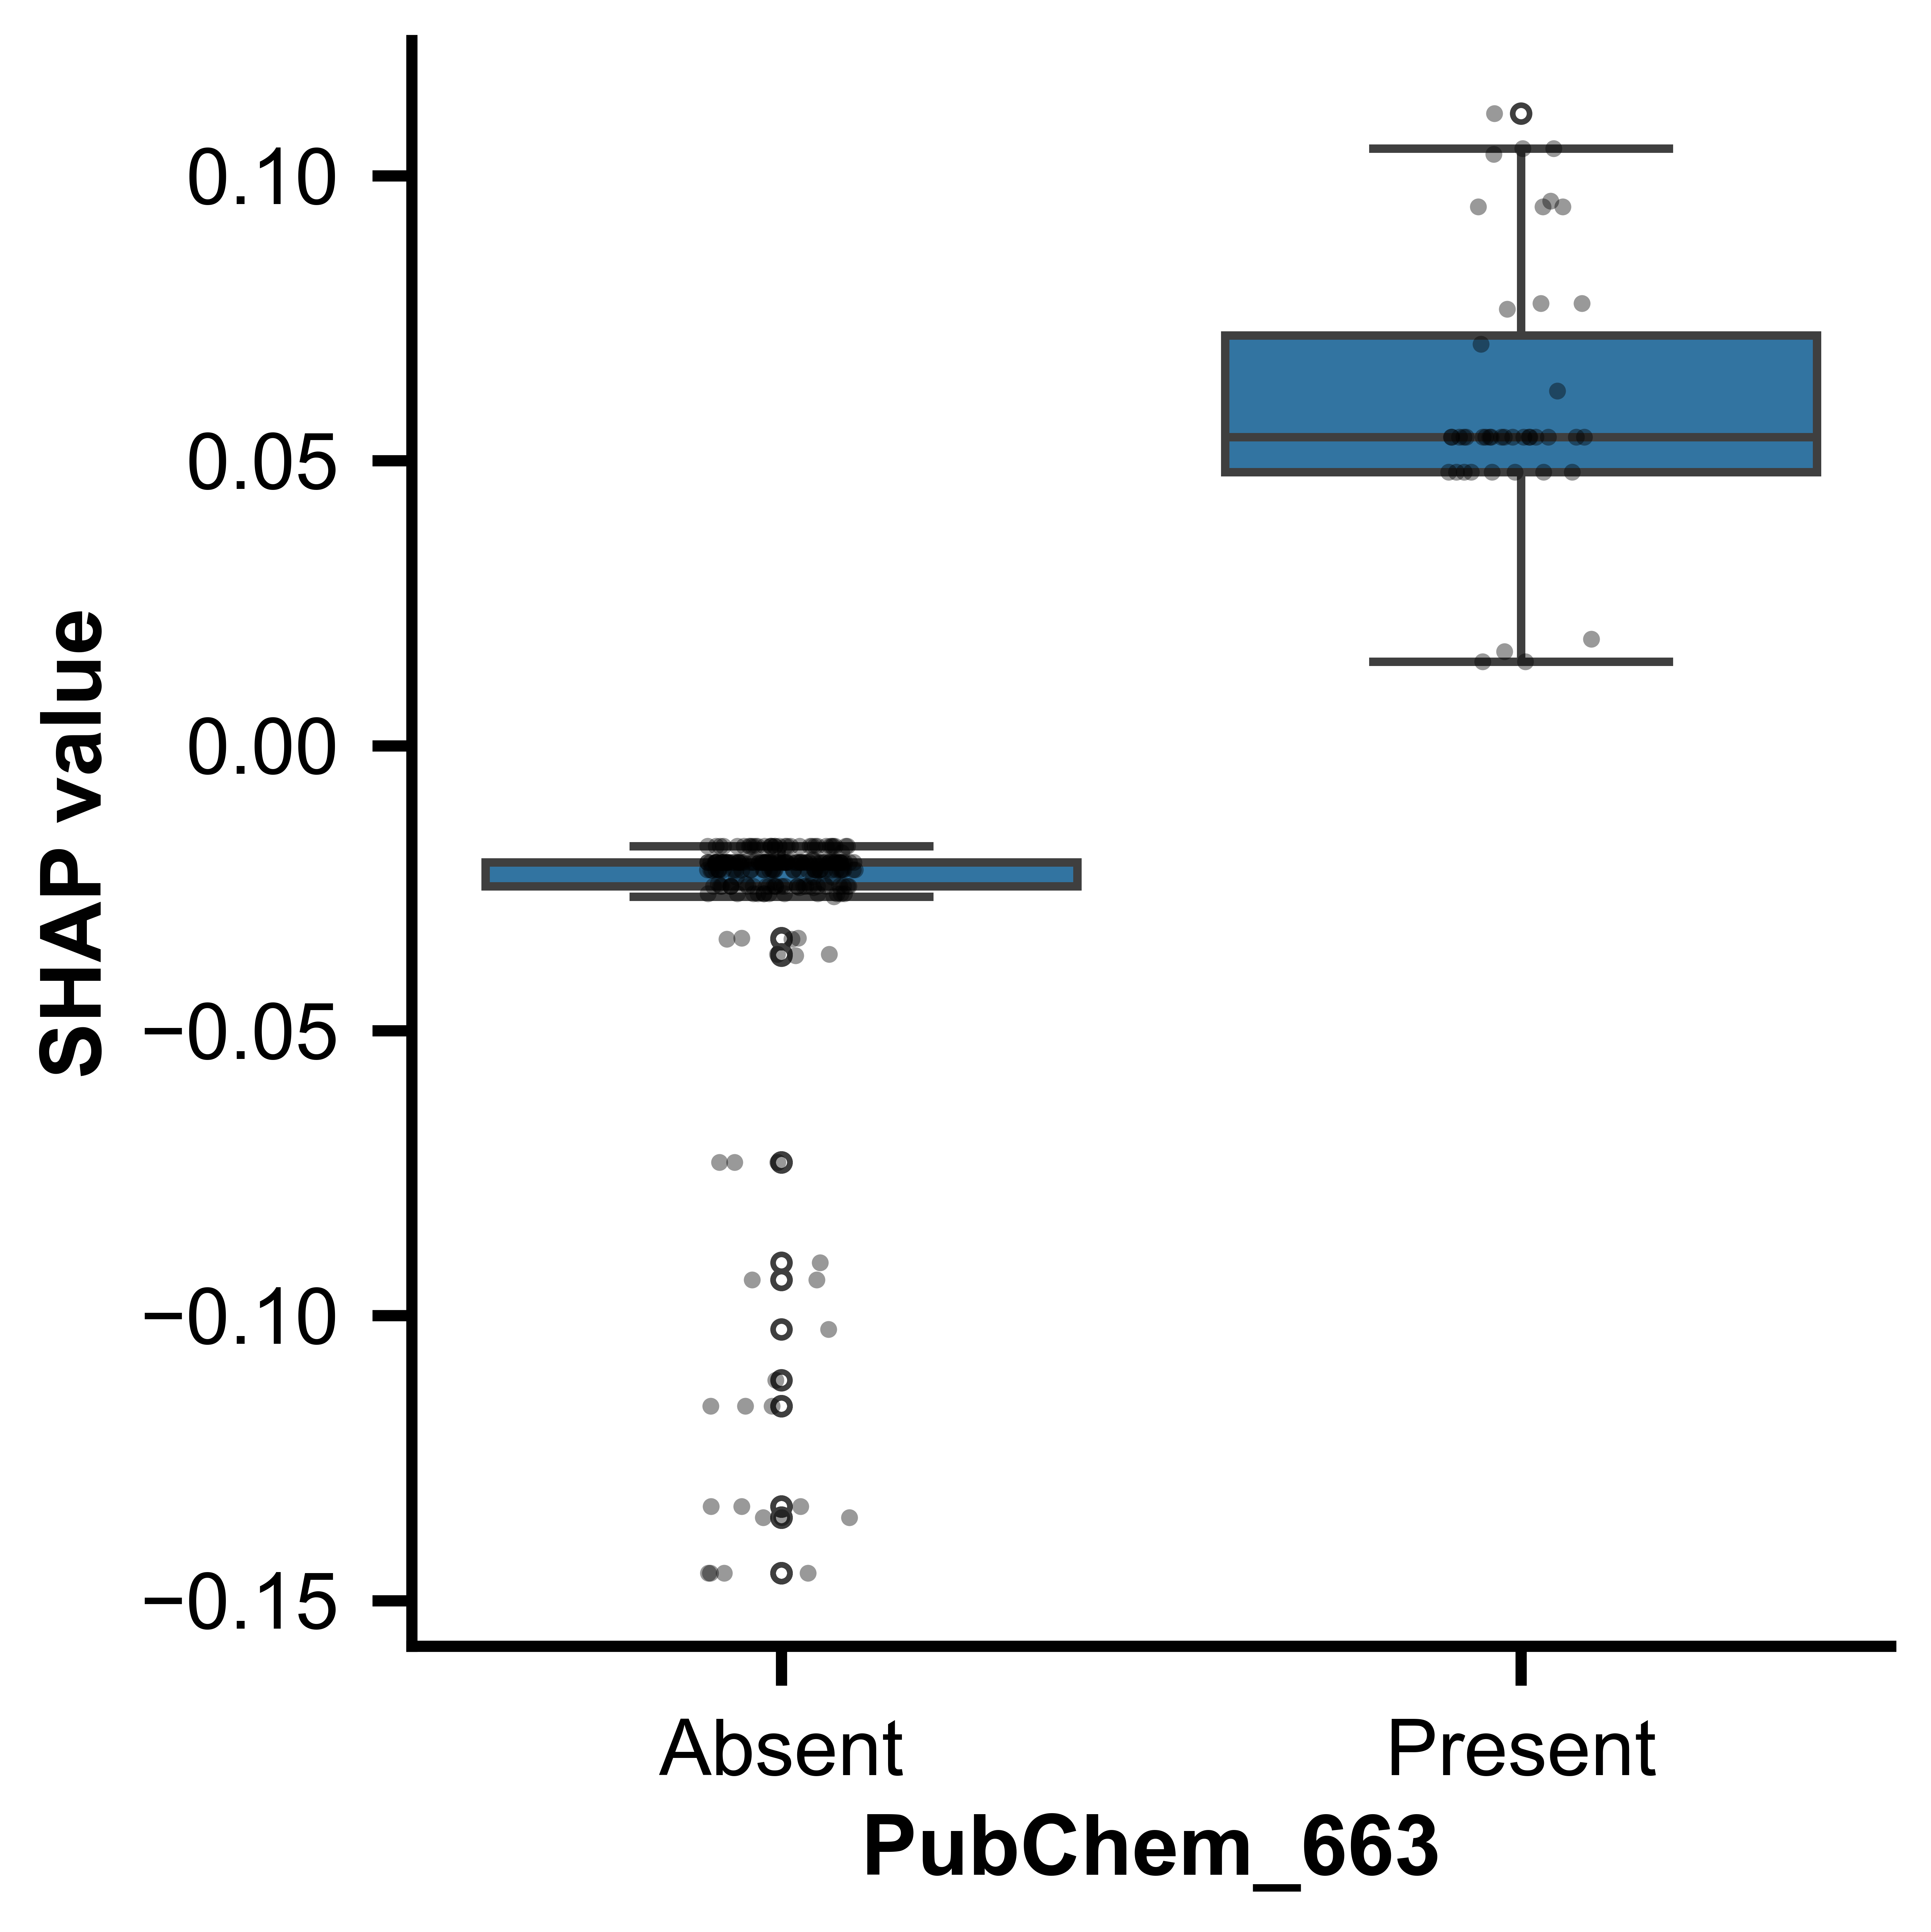
\includegraphics[width=0.43\textwidth, keepaspectratio]{prism-uploads/PubChem_663_boxplot.png} &
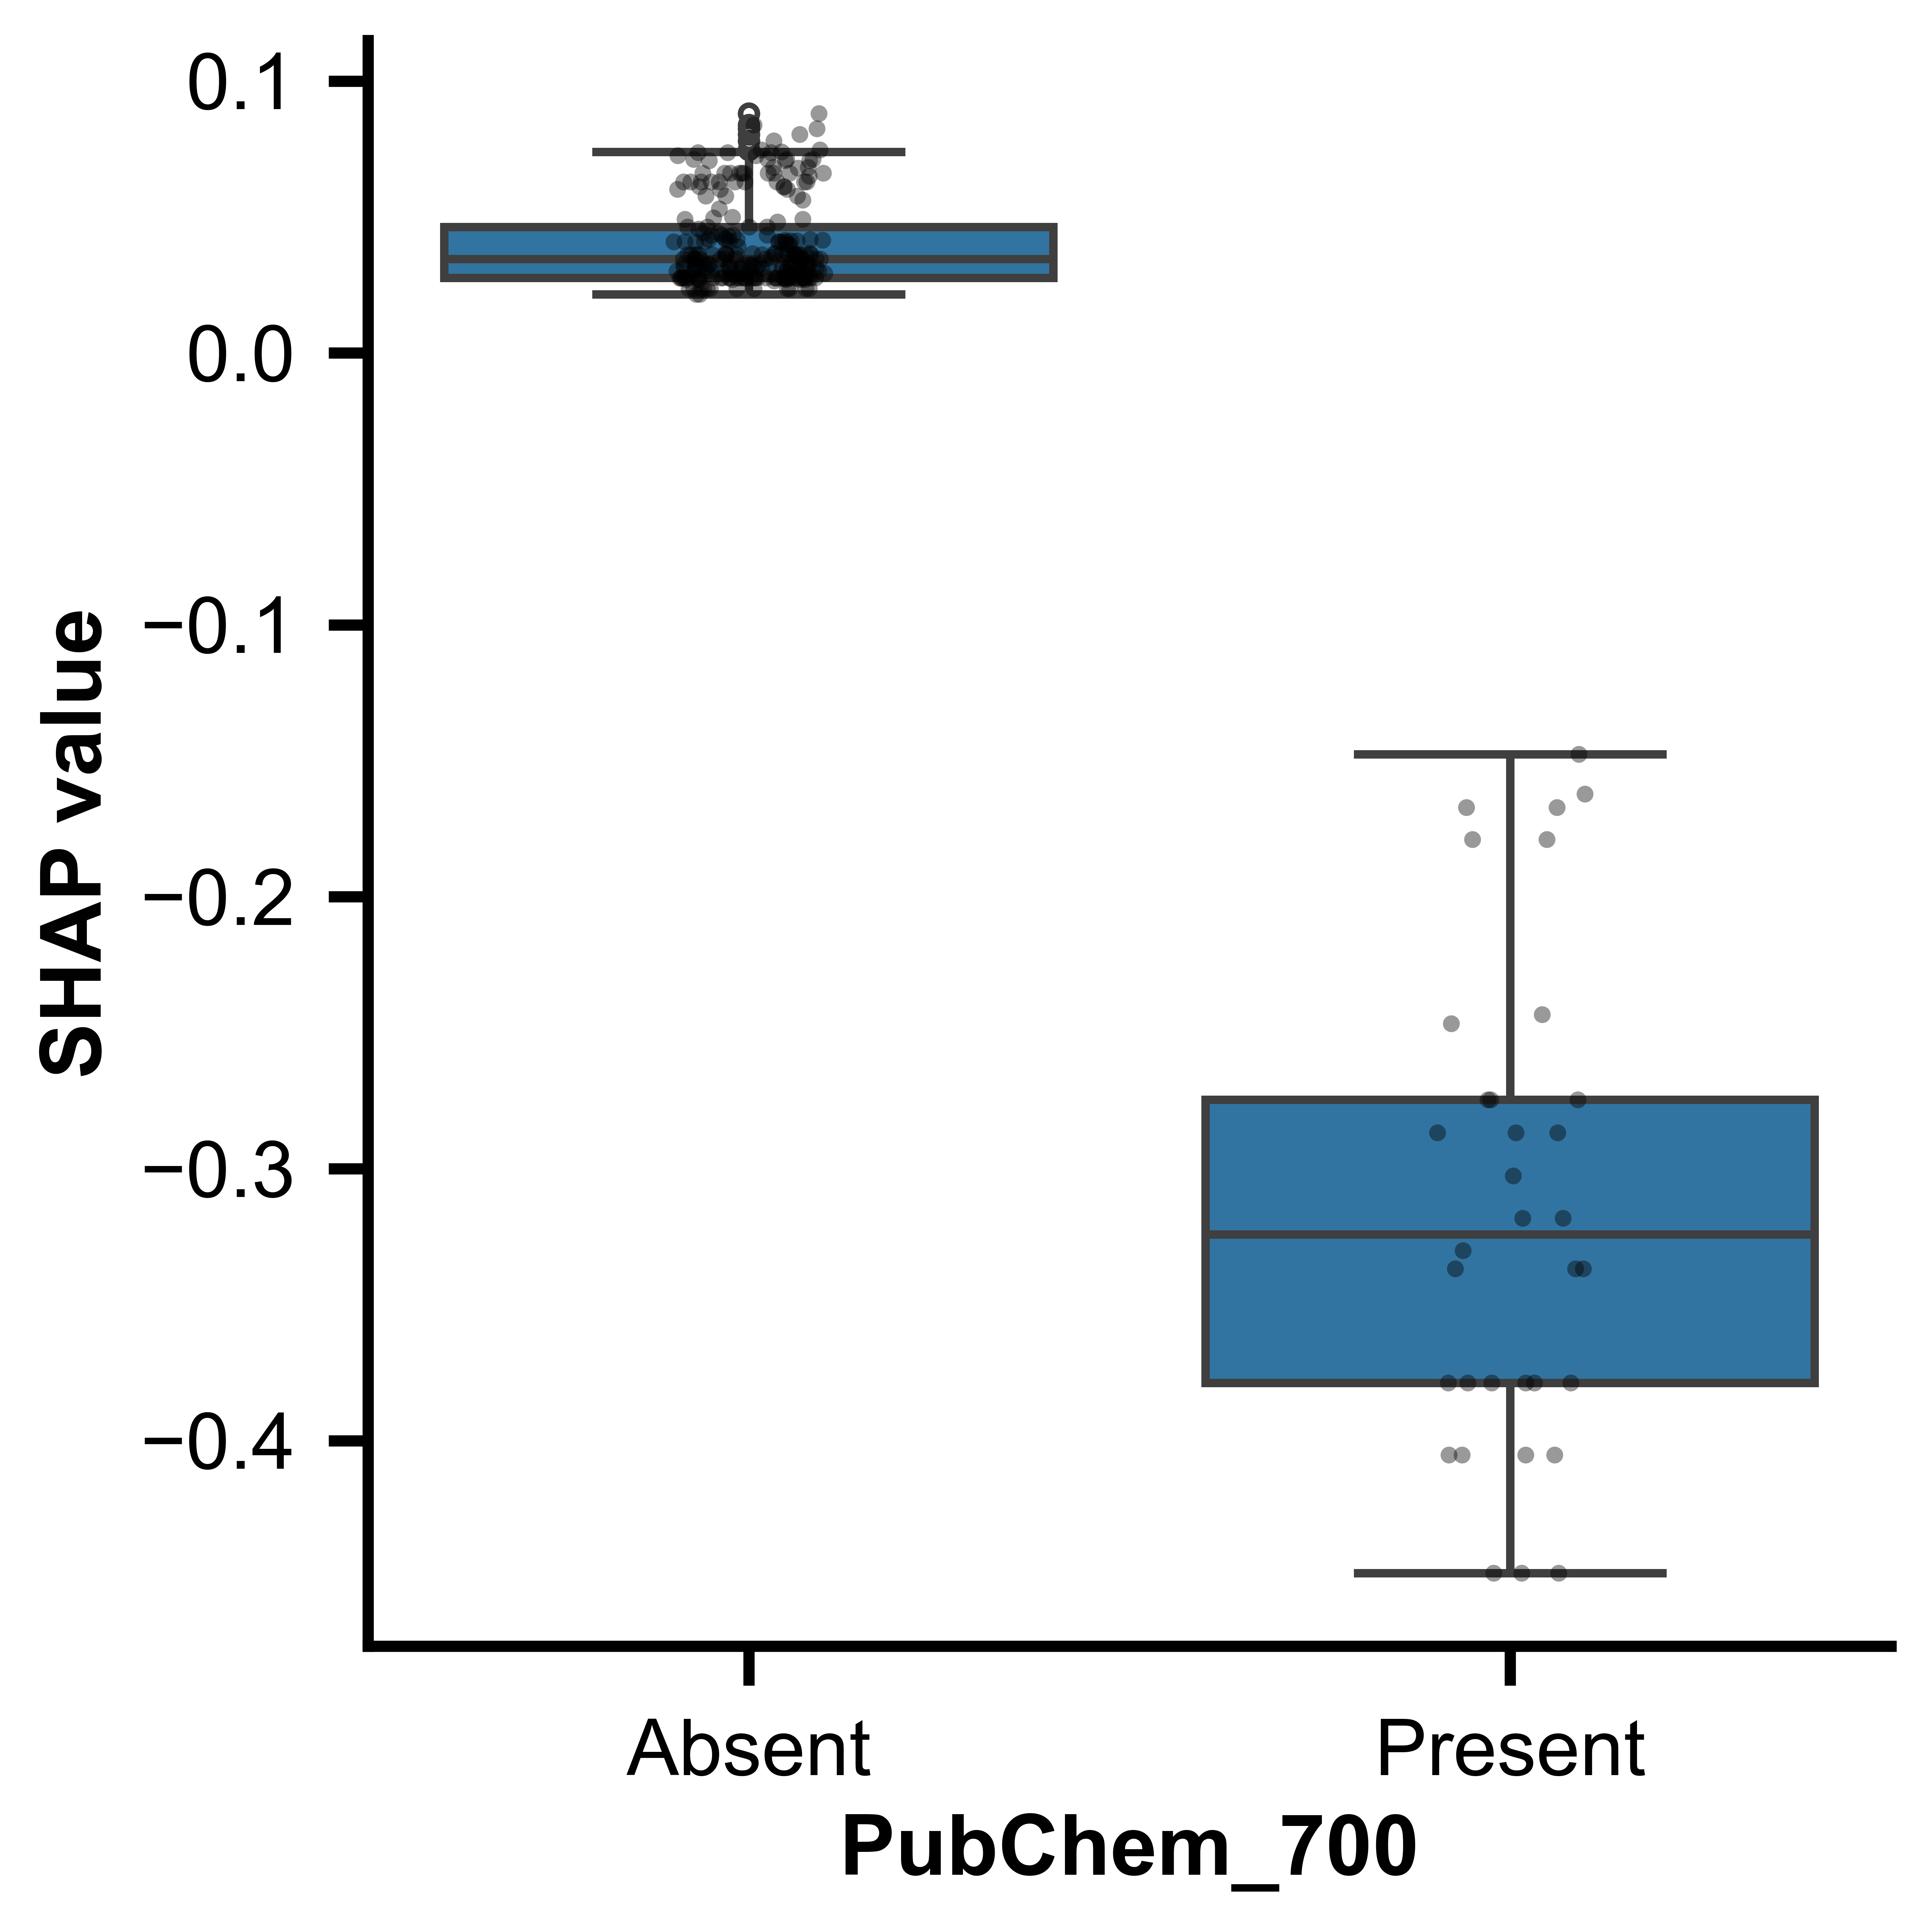
\includegraphics[width=0.43\textwidth, keepaspectratio]{prism-uploads/PubChem_700_boxplot.png} \\
(c) PubChem\_663 & (d) PubChem\_700 \\
\end{tabular}
\caption[Boxplot distributions for SHAP-ranked PubChem descriptors, part 2]{Boxplot distributions of pIC$_{50}$ values grouped by the absence or presence of selected SHAP-ranked PubChem fingerprint descriptors. Panels show PubChem\_569, PubChem\_646, PubChem\_663, and PubChem\_700.}
\label{fig:pubchem-boxplots-2}
\end{figure}

The representative-compound panel and descriptor-stratified boxplots place the SHAP-ranked fingerprints in chemical context (Figures~\ref{fig:representative-potency-structures}--\ref{fig:pubchem-boxplots-2}). These analyses translate binary fingerprint attributions into medicinal-chemistry hypotheses but do not replace prospective SAR experiments. Nitrogen-containing, carbonyl/amide-like, chlorinated, oxygenated-chain, aromatic, and diamine-like motifs should therefore be interpreted within their parent scaffolds rather than as isolated substructure rules, because urease inhibition depends on nickel coordination, hydrogen bonding, polarity modulation, and scaffold-dependent recognition.

\subsection{Applicability Domain of the Final Model}

Applicability-domain analysis identified compounds with unusual leverage or large standardized residuals in the final training descriptor matrix (Figure~\ref{fig:applicability-domain}). The analysis included 280 compounds and 135 descriptors, with a warning leverage threshold of $h^*$ = 1.4571. No compounds exceeded the warning leverage threshold. Three compounds exceeded the standardized residual limit of $+3$, whereas no compounds fell below $-3$; consequently, 277 of 280 training compounds (98.9\%) were located within the defined applicability domain under the combined leverage and standardized-residual criteria. The three response outliers warrant assay-quality review, duplicate assessment, and cautious interpretation in subsequent model deployment.

\begin{figure}[htbp]
\centering
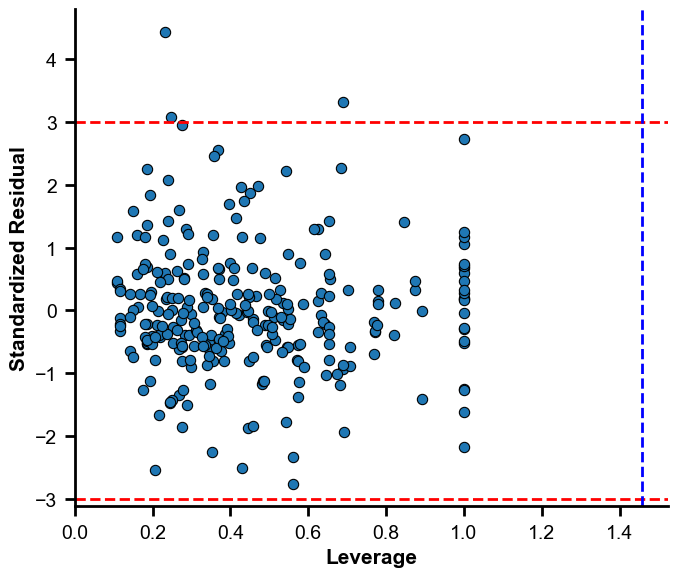
\includegraphics[width=0.82\textwidth, keepaspectratio]{prism-uploads/image_3.png}
\caption[Applicability-domain diagnostic plot]{Applicability-domain diagnostic plot for the final training dataset. The analysis used 280 compounds and 135 retained PubChem fingerprint descriptors. The blue dashed vertical line shows the warning leverage threshold ($h^* = 1.4571$), and the red dashed horizontal lines show standardized-residual warning limits at $\pm 3$.}
\label{fig:applicability-domain}
\end{figure}


\section{Discussion}

This work reports an interpretable, species-specific QSAR framework for \textit{H. pylori} urease inhibitor potency modeling. The framework integrates endpoint curation, continuous pIC$_{50}$ modeling, filtered PubChem fingerprints, external validation, OECD-style checks, Y-randomization, applicability-domain analysis, fingerprint enrichment, representative compound inspection, and SHAP interpretation within a reproducible workflow. This design supports joint assessment of prediction performance, chemical interpretation, and domain-of-use boundaries in a dataset derived from a fragmented \textit{H. pylori} urease inhibitor literature \textcolor{blue}{(Muratov et al., 2020; OECD, 2024; Tropsha, 2010)}.

The results indicate that curated \textit{H. pylori}-restricted bioactivity data, filtered molecular fingerprints, and external validation can support a regression model with independent predictive utility. HistGradientBoostingRegressor was the most defensible baseline in this dataset, consistent with the ability of boosted trees to model nonlinear combinations of sparse fingerprint bits while maintaining regularized external behavior \textcolor{blue}{(Friedman, 2001; Ke et al., 2017; Muratov et al., 2020)}.

The external behavior of HistGradientBoostingRegressor is consistent with both machine-learning and cheminformatics considerations. Gradient boosting sequentially corrects residual errors and can represent nonlinear structure--activity relationships that are difficult for linear models to express, whereas histogram-based tree construction discretizes split candidates and can reduce sensitivity to noisy thresholds in high-dimensional descriptor matrices \textcolor{blue}{(Friedman, 2001; Ke et al., 2017)}. This balance is relevant for molecular fingerprints, where many bits are sparse, correlated, or informative only in combination with other substructures. BayesianRidge and LassoLarsIC provide stable linear baselines, RandomForestRegressor reduces variance by bagging, and conventional GradientBoostingRegressor can fit stronger training or cross-validation patterns; however, their external results in this dataset were less favorable \textcolor{blue}{(Breiman, 2001; MacKay, 1992; Tibshirani, 1996; Efron et al., 2004)}. The observed ranking is therefore best interpreted as a bias--variance and representation trade-off rather than a general hierarchy of regression algorithms.

These findings align with previous ligand-based and enzyme-inhibitor modeling studies showing that nonlinear learners can be advantageous when bioactivity depends on multiple substructural motifs, while apparent performance remains strongly influenced by curation and validation design. Large ChEMBL-scale comparisons indicate that algorithmic gains can be modest relative to endpoint consistency, analogue-series bias, and train--test partitioning, and urease-focused studies similarly support descriptor-driven modeling when the biological context is carefully defined \textcolor{blue}{(Aniceto et al., 2023; Lenselink et al., 2017; Mayr et al., 2018; Morales et al., 2024; Wang et al., 2024)}. The present study differs from several prior urease modeling efforts by preserving continuous pIC$_{50}$ values, restricting the endpoint to \textit{H. pylori} urease, and applying external and randomization checks; these choices position the model as a species-specific regression benchmark rather than a classification-oriented or mixed-source urease screen \textcolor{blue}{(Fourches et al., 2010; Muratov et al., 2020)}.

\begin{table}[htbp]
\centering
\scriptsize
\setlength{\tabcolsep}{3pt}
\caption[Comparison with previous urease QSAR and machine-learning studies]{Comparison of the present model with representative urease QSAR and machine-learning studies. Direct numerical comparison should be interpreted cautiously because dataset composition, enzyme source, endpoint type, splitting strategy, and validation metrics differ among studies.}
\label{tab:previous-qSAR-comparison}
\resizebox{\textwidth}{!}{%
\begin{tabular}{p{0.18\textwidth}p{0.24\textwidth}p{0.16\textwidth}p{0.18\textwidth}p{0.20\textwidth}}
\hline
Study & Dataset/target & Endpoint & Main method & Reported test R$^2$ or closest metric \\
\hline
Zaheer-ul-Haq and Wadood (2009) & 27 hydroxamic acid urease inhibitors; not restricted to the present curated \textit{H. pylori} pIC$_{50}$ set & Urease inhibitory potency & Docking plus 3D-QSAR CoMFA/CoMSIA & No comparable random-split test R$^2$; LOO q$^2$ = 0.848/0.755 and r$^2$ = 0.978/0.984 for CoMFA/CoMSIA \\
Aniceto et al. (2023) & Urease inhibition data integrated with molecular docking for virtual screening & Activity prioritization and screening & Machine learning plus docking & No comparable pIC$_{50}$ test R$^2$; reported for virtual-screening prioritization rather than species-specific regression \\
Morales et al. (2024) & Urease inhibitor dataset filtered by physicochemical properties & Binary urease-inhibitor classification & Supervised classification models & No regression test R$^2$ because the endpoint was classification; useful comparator for screening filters rather than continuous potency prediction \\
Wang et al. (2024) & Hydroxamic acid-based \textit{H. pylori} urease inhibitor design set & Continuous potency prediction with docking and molecular dynamics follow-up & Ensemble learning model & Reported R$^2$ = 0.761 for a focused hydroxamic acid domain; complementary to this broader workflow \\
Present study & 351 curated \textit{H. pylori} urease IC$_{50}$ records; 280/71 random train--test split & Continuous pIC$_{50}$ regression & HistGradientBoosting with PubChem fingerprints, OECD checks, Y-randomization, SHAP, and AD analysis & R$^2_{test}$ = 0.712; R$^2_{ext}$ = 0.714; RMSE$_{test}$ = 0.506; MAE$_{test}$ = 0.375 \\
\hline
\end{tabular}%
}
\end{table}

Model reliability depends on the data-processing steps as well as the regression algorithm. ChEMBL provides a high-quality starting point for ligand--target bioactivity modeling, but public bioactivity records still require endpoint filtering, duplicate reconciliation, unit harmonization, and structure standardization before QSAR inference \textcolor{blue}{(Fourches et al., 2010; Zdrazil et al., 2024)}. Transforming IC$_{50}$ values to pIC$_{50}$ placed the response on a logarithmic potency scale, while PubChem fingerprints converted structures into reproducible substructure descriptors suitable for ligand-based learning \textcolor{blue}{(Kim et al., 2023; Willett, 2006)}. Variance filtering removed uninformative bits, and correlation filtering reduced redundant descriptor families, thereby lowering noise, improving numerical stability, and reducing duplicated structural signal \textcolor{blue}{(Cereto-Massague et al., 2015; Guyon \& Elisseeff, 2003)}.

Each validation layer addresses a different failure mode in QSAR modeling. Five-fold cross-validation estimates training-set stability under resampling, but it cannot by itself establish external transferability when related analogues or assay-specific patterns are unevenly distributed across folds \textcolor{blue}{(Mayr et al., 2018; Tropsha, 2010)}. The independent test set provides a more relevant assessment of held-out prediction, whereas the Golbraikh--Tropsha/OECD-style statistics examine proportionality and bias in external QSAR predictions \textcolor{blue}{(Golbraikh \& Tropsha, 2002; OECD, 2024)}. Y-randomization adds a negative control by disrupting the structure--activity mapping; the loss of external predictive behavior in randomized models supports that the retained signal was not solely a chance correlation produced by descriptor dimensionality or model flexibility \textcolor{blue}{(Rucker et al., 2007; Tropsha, 2010)}.

The RandomizedSearchCV optimization result cautions against selecting QSAR models solely by internal resampling performance. Although hyperparameter search improved the mean cross-validation score, the corresponding decrease in independent external predictivity suggests that the optimized configuration captured fold-specific structure--activity regularities that did not generalize to held-out compounds. This pattern is consistent with model-selection bias, in which repeated evaluation over hyperparameter combinations overfits the validation procedure itself, especially in modest chemical datasets with clustered analogue series \textcolor{blue}{(Bergstra \& Bengio, 2012; Cawley \& Talbot, 2010; Mayr et al., 2018)}. Retaining the default HistGradientBoostingRegressor was therefore justified by the external predictive criterion used in this baseline QSAR analysis \textcolor{blue}{(Muratov et al., 2020; OECD, 2024; Tropsha, 2010)}.

The chemical interpretation remains ligand-based and fingerprint-mediated rather than mechanistic. PubChem fingerprint bits encode predefined structural patterns, so the learned relationships most likely reflect combinations of substructures associated with reported \textit{H. pylori} urease potency rather than explicit binding mechanisms \textcolor{blue}{(Kim et al., 2023; Willett, 2006)}. This representation is suitable for a baseline QSAR model because urease inhibitors span hydroxamate, heterocyclic, selenium-containing, sulfur-containing, and natural-product-derived chemotypes, many of which contain functional groups associated with metal coordination, covalent reactivity, hydrogen bonding, or scaffold-dependent recognition \textcolor{blue}{(Chen et al., 2025; Guzel-Akdemir \& Akdemir, 2025; Kafarski \& Talma, 2018; Wang et al., 2024)}. SHAP-ranked fingerprint descriptors should therefore be treated as interpretable correlates, not causal pharmacophores, unless supported by matched molecular-pair analysis, docking, experimental perturbation, or prospective analogue testing.

The interpreted SHAP analysis connects HistGradientBoosting predictions to descriptor-level attributions rather than treating the model as an opaque screening engine. The leading descriptors mapped to chemically meaningful PubChem definitions, including nitrogen-containing, carbonyl chain, amide-like, chlorinated, oxygenated chain, aromatic carbon, and diamine-like patterns. These assignments provide a rational basis for inspecting chemical series that drive model predictions while avoiding unsupported claims of direct binding causality. Such explainable modeling can reveal whether predictions are driven by chemically interpretable descriptor patterns and can support compound prioritization before synthesis or biological testing \textcolor{blue}{(Jimenez-Luna et al., 2020; Lundberg \& Lee, 2017; Lundberg et al., 2020; Rodriguez-Perez \& Bajorath, 2020)}.

The strongest SHAP signals are consistent with established urease medicinal chemistry. Nitrogen-containing descriptors such as PubChem\_14 and diamine-like PubChem\_569 may reflect ligands with atoms capable of protonation, hydrogen bonding, or metal-associated interactions near the dinuclear Ni$^{2+}$ urease active site, although the fingerprint itself does not specify coordination geometry. Carbonyl chain and amide-like descriptors such as PubChem\_535, PubChem\_646, and PubChem\_439 may capture carbonyl oxygen atoms and adjacent heteroatoms that orient inhibitors through hydrogen-bonding or metal-proximal interactions, especially in hydroxamate-like or amide-containing urease inhibitor families. Chlorinated and aromatic carbon descriptors may encode lipophilicity, electronic modulation, and scaffold packing effects, whereas oxygenated chain descriptors may capture polarity and hydrogen-bonding patterns. These interpretations are consistent with structural and medicinal-chemistry knowledge of \textit{H. pylori} urease inhibition, where potency can depend on nickel-directed functionality, heteroatom placement, and scaffold context rather than on a single isolated substructure \textcolor{blue}{(Cunha et al., 2021; Ha et al., 2001; Kafarski \& Talma, 2018; Wang et al., 2024)}.

The model is best used as a triage tool within the chemical domain represented by the curated dataset. In virtual screening, it can rank candidate \textit{H. pylori} urease inhibitors before experimental testing and prioritize scaffolds with a higher predicted probability of favorable potency \textcolor{blue}{(Lavecchia, 2015; Stokes et al., 2020)}. For lead optimization, predictions should be considered alongside chemical feasibility, selectivity, assay quality, and ADMET criteria rather than used as standalone decision criteria \textcolor{blue}{(Daina et al., 2017; Jimenez-Luna et al., 2020)}. These applications remain preclinical and require prospective biochemical validation.

A major strength of the study is the combination of endpoint discipline, descriptor transparency, and multiple validation safeguards. Restricting the endpoint to \textit{H. pylori} urease reduces biological confounding from surrogate enzymes, while duplicate removal, pIC$_{50}$ standardization, fingerprint filtering, explicit train--test separation, applicability-domain analysis, and interpretable descriptor ranking improve reproducibility and auditability. Cross-validation, independent external validation, OECD/Golbraikh--Tropsha statistics, and Y-randomization collectively assess internal stability, external predictivity, proportionality of predictions, and resistance to chance correlation \textcolor{blue}{(Golbraikh \& Tropsha, 2002; Muratov et al., 2020; OECD, 2024; Rucker et al., 2007)}. These features support the workflow as a baseline for subsequent optimization and interpretation.

Several limitations define the domain of interpretation. The dataset remains modest and dependent on available ChEMBL and literature bioactivity records; residual assay heterogeneity, uneven scaffold representation, and publication bias may therefore persist despite curation. The model is also single-target and ligand-based and does not account for bacterial uptake, compound stability, off-target antibacterial mechanisms, cytotoxicity, or pharmacokinetic liabilities. The 80/20 random split provides an independent held-out test set but may overestimate prospective performance when close analogues occur in both partitions; scaffold-aware Bemis--Murcko splitting or temporal validation remains an important next validation layer \textcolor{blue}{(Bemis \& Murcko, 1996; Mayr et al., 2018; Tropsha, 2010)}. The leverage-based applicability-domain analysis provides an initial diagnostic for high-leverage and residual outlier compounds, although leverage diagnostics do not fully capture scaffold novelty, assay heterogeneity, or mechanistic uncertainty \textcolor{blue}{(Sahigara et al., 2013; Tropsha, 2010)}. Prediction intervals, conformal prediction, ensemble variance, or related uncertainty estimates would further strengthen prioritization decisions.

Future work should extend this baseline with validation designs and uncertainty estimates that better assess prospective transferability. Scaffold-aware splitting, repeated external validation, expanded applicability-domain analysis, SHAP dependence/interaction plots, and uncertainty estimation would clarify chemical-series generalization before deployment. Transfer learning and graph neural networks may become informative as larger urease and antibacterial datasets are assembled, particularly for representing molecular topology beyond fixed fingerprint bits \textcolor{blue}{(Altae-Tran et al., 2017; Yang et al., 2019)}. Explainable AI, active learning, and generative molecular design may guide analogue selection, chemotype proposal, and compound prioritization when coupled to prospective biochemical testing \textcolor{blue}{(Jimenez-Luna et al., 2020; Lundberg et al., 2020; Sanchez-Lengeling \& Aspuru-Guzik, 2018; Warmuth et al., 2003)}. Integration with molecular docking, molecular dynamics simulations, and ADMET prediction would further help separate ligand-based potency signals from binding feasibility, selectivity, and developability constraints \textcolor{blue}{(Daina et al., 2017; Wang et al., 2024)}.

Overall, this study presents an interpretable, species-specific QSAR framework for predicting \textit{H. pylori} urease inhibitor potency using explainable machine learning, endpoint curation, external validation, OECD-style diagnostic checks, Y-randomization, and applicability-domain assessment. The framework links potency prediction with chemically meaningful fingerprint patterns and explicit deployment boundaries. HistGradientBoostingRegressor provided the strongest balance between nonlinear learning and external generalization in the current dataset, supporting its use as a baseline for applicability-domain-aware virtual screening, scaffold-focused validation, and experimentally guided anti-\textit{H. pylori} lead optimization.

\section*{Code and Data Availability}

Curated modeling data, train--test partitions, model-comparison outputs, validation summaries, feature-attribution tables, applicability-domain diagnostics, and analysis scripts will be provided as Supplementary Data or through a version-controlled repository at submission.

\section*{References}

Altae-Tran, H., Ramsundar, B., Pappu, A. S., \& Pande, V. (2017). Low data drug discovery with one-shot learning. \textit{ACS Central Science, 3}(4), 283--293. \url{https://doi.org/10.1021/acscentsci.6b00367}

Aniceto, N., Albuquerque, T. S., Bonifacio, V. D. B., Guedes, R. C., \& Martinho, N. (2023). Using machine learning and molecular docking to leverage urease inhibition data for virtual screening. \textit{International Journal of Molecular Sciences, 24}(9), 8180. \url{https://doi.org/10.3390/ijms24098180}

Bemis, G. W., \& Murcko, M. A. (1996). The properties of known drugs. 1. Molecular frameworks. \textit{Journal of Medicinal Chemistry, 39}(15), 2887--2893. \url{https://doi.org/10.1021/jm9602928}

Bergstra, J., \& Bengio, Y. (2012). Random search for hyper-parameter optimization. \textit{Journal of Machine Learning Research, 13}, 281--305.

Breiman, L. (2001). Random forests. \textit{Machine Learning, 45}, 5--32. \url{https://doi.org/10.1023/A:1010933404324}

Cao, W., Jin, F., Liu, B., Xu, G., Jin, S., Jia, Z., Peng, P., Song, W., Li, F., Gao, D., \& Feng, K. (2025). Synthesis and evaluation of novel ebselen derivatives as urease inhibitors for combating \textit{Helicobacter pylori} infections. \textit{European Journal of Medicinal Chemistry, 287}, 117359. \url{https://doi.org/10.1016/j.ejmech.2025.117359}

Cardos, I. A., Danila, C., Yahya, G., Seleem, N. M., Mosbah, R. A., Shaldam, M. A., Vicas, S. I., Metwally, K., \& Cavalu, S. D. (2026). Targeting \textit{Helicobacter pylori} enzymes using \textit{Viscum album} L. extract: In silico molecular docking and in vitro study. \textit{Frontiers in Cellular and Infection Microbiology, 15}, 1690969. \url{https://doi.org/10.3389/fcimb.2025.1690969}

Cesareo, S. D., \& Langton, S. R. (1992). Kinetic properties of \textit{Helicobacter pylori} urease compared with jack bean urease. \textit{FEMS Microbiology Letters, 99}(1), 15--21. \url{https://doi.org/10.1111/j.1574-6968.1992.tb05535.x}

Chawla, N. V., Bowyer, K. W., Hall, L. O., \& Kegelmeyer, W. P. (2002). SMOTE: Synthetic minority over-sampling technique. \textit{Journal of Artificial Intelligence Research, 16}, 321--357. \url{https://doi.org/10.1613/jair.953}

Cawley, G. C., \& Talbot, N. L. C. (2010). On over-fitting in model selection and subsequent selection bias in performance evaluation. \textit{Journal of Machine Learning Research, 11}, 2079--2107.

Cereto-Massague, A., Ojeda, M. J., Valls, C., Mulero, M., Garcia-Vallve, S., \& Pujadas, G. (2015). Molecular fingerprint similarity search in virtual screening. \textit{Methods, 71}, 58--63. \url{https://doi.org/10.1016/j.ymeth.2014.08.005}

Chen, X., Gou, L., Wang, Y., Yang, J., Dong, Y., Xie, B., \& Zhang, D. (2025). New directions in \textit{Helicobacter pylori} urease inhibitors: Focusing on nickel ions transfer and auxiliary protein interactions during urease maturation. \textit{Infection and Drug Resistance, 18}, 3037--3053. \url{https://doi.org/10.2147/IDR.S519194}

Chen, T., \& Guestrin, C. (2016). XGBoost: A scalable tree boosting system. In \textit{Proceedings of the 22nd ACM SIGKDD International Conference on Knowledge Discovery and Data Mining} (pp. 785--794). \url{https://doi.org/10.1145/2939672.2939785}

Chicco, D., Warrens, M. J., \& Jurman, G. (2021). The coefficient of determination R-squared is more informative than SMAPE, MAE, MAPE, MSE and RMSE in regression analysis evaluation. \textit{PeerJ Computer Science, 7}, Article e623. \url{https://doi.org/10.7717/peerj-cs.623}

Cortes, C., \& Vapnik, V. (1995). Support-vector networks. \textit{Machine Learning, 20}, 273--297. \url{https://doi.org/10.1007/BF00994018}

Crowe, S. E. (2019). \textit{Helicobacter pylori} infection. \textit{New England Journal of Medicine, 380}(12), 1158--1165. \url{https://doi.org/10.1056/NEJMcp1710945}

Cunha, E. S., Chen, X., Sanz-Gaitero, M., Mills, D. J., Luecke, H., \& Imkamp, F. (2021). Cryo-EM structure of \textit{Helicobacter pylori} urease with an inhibitor in the active site at 2.0~\AA{} resolution. \textit{Nature Communications, 12}, Article 230. \url{https://doi.org/10.1038/s41467-020-20485-6}

Davis, J., \& Goadrich, M. (2006). The relationship between precision-recall and ROC curves. In \textit{Proceedings of the 23rd International Conference on Machine Learning} (pp. 233--240). \url{https://doi.org/10.1145/1143844.1143874}

Daina, A., Michielin, O., \& Zoete, V. (2017). SwissADME: A free web tool to evaluate pharmacokinetics, drug-likeness and medicinal chemistry friendliness of small molecules. \textit{Scientific Reports, 7}, Article 42717. \url{https://doi.org/10.1038/srep42717}

Efron, B., Hastie, T., Johnstone, I., \& Tibshirani, R. (2004). Least angle regression. \textit{The Annals of Statistics, 32}(2), 407--499. \url{https://doi.org/10.1214/009053604000000067}

Fawcett, T. (2006). An introduction to ROC analysis. \textit{Pattern Recognition Letters, 27}(8), 861--874. \url{https://doi.org/10.1016/j.patrec.2005.10.010}

Friedman, J. H. (2001). Greedy function approximation: A gradient boosting machine. \textit{The Annals of Statistics, 29}(5), 1189--1232. \url{https://doi.org/10.1214/aos/1013203451}

Golbraikh, A., \& Tropsha, A. (2002). Beware of q$^2$! \textit{Journal of Molecular Graphics and Modelling, 20}(4), 269--276. \url{https://doi.org/10.1016/S1093-3263(01)00123-1}

Fourches, D., Muratov, E., \& Tropsha, A. (2010). Trust, but verify: On the importance of chemical structure curation in cheminformatics and QSAR modeling research. \textit{Journal of Chemical Information and Modeling, 50}(7), 1189--1204. \url{https://doi.org/10.1021/ci100176x}

Guyon, I., \& Elisseeff, A. (2003). An introduction to variable and feature selection. \textit{Journal of Machine Learning Research, 3}, 1157--1182.

Grabarek, M., Tabor, W., Krzyzek, P., Bakowicz, J., Grabowiecka, A., Berlicki, L., \& Mucha, A. (2025). Synthesis of phosphonate derivatives of benzisoselenazolones and their remarkable antiureolytic activity in \textit{Helicobacter pylori} cells. \textit{Journal of Medicinal Chemistry, 68}(19), 20324--20339. \url{https://doi.org/10.1021/acs.jmedchem.5c01385}

Guzel-Akdemir, O., \& Akdemir, A. (2025). Urease inhibitors for the treatment of \textit{H. pylori}. \textit{Expert Opinion on Therapeutic Patents, 35}(1), 17--30. \url{https://doi.org/10.1080/13543776.2024.2423004}

Ha, N.-C., Oh, S.-T., Sung, J. Y., Cha, K. A., Lee, M. H., \& Oh, B.-H. (2001). Supramolecular assembly and acid resistance of \textit{Helicobacter pylori} urease. \textit{Nature Structural Biology, 8}(6), 505--509. \url{https://doi.org/10.1038/88563}

Jimenez-Luna, J., Grisoni, F., \& Schneider, G. (2020). Drug discovery with explainable artificial intelligence. \textit{Nature Machine Intelligence, 2}(10), 573--584. \url{https://doi.org/10.1038/s42256-020-00236-4}

Kafarski, P., \& Talma, M. (2018). Recent advances in design of new urease inhibitors: A review. \textit{Journal of Advanced Research, 13}, 101--112. \url{https://doi.org/10.1016/j.jare.2018.01.007}

Ke, G., Meng, Q., Finley, T., Wang, T., Chen, W., Ma, W., Ye, Q., \& Liu, T.-Y. (2017). LightGBM: A highly efficient gradient boosting decision tree. In \textit{Advances in Neural Information Processing Systems 30} (pp. 3146--3154).

Khoder, G., Mustafa, E. M., Zaib, S., Ravi, A., Shahin, A. I., Zaraei, S.-O., Rana, N., Anbar, H. S., Ali, H. S., Qumar, S., Sebastian, M., Alsheikh Zein, R., \& El-Gamal, M. I. (2026). Novel indole-based sulfonate and sulfamate derivatives as potent and selective urease inhibitors targeting \textit{Helicobacter pylori}: A promising therapeutic strategy. \textit{Gut Pathogens, 18}, Article 27. \url{https://doi.org/10.1186/s13099-026-00814-8}

Kim, S., Chen, J., Cheng, T., Gindulyte, A., He, J., He, S., Li, Q., Shoemaker, B. A., Thiessen, P. A., Yu, B., Zaslavsky, L., Zhang, J., \& Bolton, E. E. (2023). PubChem 2023 update. \textit{Nucleic Acids Research, 51}(D1), D1373--D1380. \url{https://doi.org/10.1093/nar/gkac956}

Li, Y., Choi, H., Leung, K., Jiang, F., Graham, D. Y., \& Leung, W. K. (2023). Global prevalence of \textit{Helicobacter pylori} infection between 1980 and 2022: A systematic review and meta-analysis. \textit{The Lancet Gastroenterology \& Hepatology, 8}(6), 553--564. \url{https://doi.org/10.1016/S2468-1253(23)00070-5}

Lavecchia, A. (2015). Machine-learning approaches in drug discovery: Methods and applications. \textit{Drug Discovery Today, 20}(3), 318--331. \url{https://doi.org/10.1016/j.drudis.2014.10.012}

Lenselink, E. B., Ten Dijke, N., Bongers, B., Papadatos, G., van Vlijmen, H. W. T., Kowalczyk, W., IJzerman, A. P., \& van Westen, G. J. P. (2017). Beyond the hype: Deep neural networks outperform established methods using a ChEMBL bioactivity benchmark set. \textit{Journal of Cheminformatics, 9}, Article 45. \url{https://doi.org/10.1186/s13321-017-0232-0}

Lundberg, S. M., \& Lee, S.-I. (2017). A unified approach to interpreting model predictions. In \textit{Advances in Neural Information Processing Systems 30} (pp. 4765--4774).

Lundberg, S. M., Erion, G., Chen, H., DeGrave, A., Prutkin, J. M., Nair, B., Katz, R., Himmelfarb, J., Bansal, N., \& Lee, S.-I. (2020). From local explanations to global understanding with explainable AI for trees. \textit{Nature Machine Intelligence, 2}(1), 56--67. \url{https://doi.org/10.1038/s42256-019-0138-9}

MacKay, D. J. C. (1992). Bayesian interpolation. \textit{Neural Computation, 4}(3), 415--447. \url{https://doi.org/10.1162/neco.1992.4.3.415}

Malfertheiner, P., Megraud, F., Rokkas, T., Gisbert, J. P., Liou, J.-M., Schulz, C., Gasbarrini, A., Hunt, R. H., Leja, M., O'Morain, C., Rugge, M., Suerbaum, S., Tilg, H., Sugano, K., \& El-Omar, E. M. (2022). Management of \textit{Helicobacter pylori} infection: The Maastricht VI/Florence consensus report. \textit{Gut, 71}(9), 1724--1762. \url{https://doi.org/10.1136/gutjnl-2022-327745}

Mayr, A., Klambauer, G., Unterthiner, T., \& Hochreiter, S. (2018). Deep learning on large-scale drug discovery data. \textit{Journal of Chemical Information and Modeling, 58}(7), 1329--1343. \url{https://doi.org/10.1021/acs.jcim.7b00572}

Morales, N., Valdes-Munoz, E., Gonzalez, J., Valenzuela-Hormazabal, P., Palma, J. M., Galarza, C., Catagua-Gonzalez, A., Yanez, O., Pereira, A., \& Bustos, D. (2024). Machine learning-driven classification of urease inhibitors leveraging physicochemical properties as effective filter criteria. \textit{International Journal of Molecular Sciences, 25}(8), 4303. \url{https://doi.org/10.3390/ijms25084303}

Muratov, E. N., Bajorath, J., Sheridan, R. P., Tetko, I. V., Filimonov, D., Poroikov, V. V., Oprea, T. I., Baskin, I. I., Varnek, A., Roitberg, A. E., Isayev, O., Curtalolo, S., Fourches, D., Cohen, Y., Aspuru-Guzik, A., Winkler, D. A., Agrafiotis, D. K., Cherkasov, A. R., \& Tropsha, A. (2020). QSAR without borders. \textit{Chemical Society Reviews, 49}(11), 3525--3564. \url{https://doi.org/10.1039/D0CS00098A}

OECD. (2024). \textit{(Q)SAR assessment framework: Guidance for the regulatory assessment of (quantitative) structure activity relationship models and predictions} (Second edition). OECD. \url{https://www.oecd.org/content/dam/oecd/en/publications/reports/2024/11/q-sar-assessment-framework-guidance-for-the-regulatory-assessment-of-quantitative-structure-activity-relationship-models-and-predictions-second-edition_cc89955e/bbdac345-en.pdf}

Odake, S., Morikawa, T., Tsuchiya, M., Imamura, L., Kobashi, K., \& Ohta, H. (1994). Inhibition of \textit{Helicobacter pylori} urease activity by hydroxamic acid derivatives. \textit{Biological and Pharmaceutical Bulletin, 17}(10), 1329--1332. \url{https://doi.org/10.1248/bpb.17.1329}

Rogers, D., \& Hahn, M. (2010). Extended-connectivity fingerprints. \textit{Journal of Chemical Information and Modeling, 50}(5), 742--754. \url{https://doi.org/10.1021/ci100050t}

Rodriguez-Perez, R., \& Bajorath, J. (2020). Interpretation of machine learning models using Shapley values: Application to compound potency and multi-target activity predictions. \textit{Journal of Computer-Aided Molecular Design, 34}, 1013--1026. \url{https://doi.org/10.1007/s10822-020-00314-0}

Rucker, C., Rucker, G., \& Meringer, M. (2007). Y-randomization and its variants in QSPR/QSAR. \textit{Journal of Chemical Information and Modeling, 47}(6), 2345--2357. \url{https://doi.org/10.1021/ci700157b}

Sachs, G., Weeks, D. L., Melchers, K., \& Scott, D. R. (2003). The gastric biology of \textit{Helicobacter pylori}. \textit{Annual Review of Physiology, 65}, 349--369. \url{https://doi.org/10.1146/annurev.physiol.65.092101.142156}

Sahigara, F., Mansouri, K., Ballabio, D., Mauri, A., Consonni, V., \& Todeschini, R. (2013). Comparison of different approaches to define the applicability domain of QSAR models. \textit{Molecules, 18}(5), 4791--4810. \url{https://doi.org/10.3390/molecules18054791}

Savoldi, A., Carrara, E., Graham, D. Y., Conti, M., \& Tacconelli, E. (2018). Prevalence of antibiotic resistance in \textit{Helicobacter pylori}: A systematic review and meta-analysis in World Health Organization regions. \textit{Gastroenterology, 155}(5), 1372--1382.e17. \url{https://doi.org/10.1053/j.gastro.2018.07.007}

Sanchez-Lengeling, B., \& Aspuru-Guzik, A. (2018). Inverse molecular design using machine learning: Generative models for matter engineering. \textit{Science, 361}(6400), 360--365. \url{https://doi.org/10.1126/science.aat2663}

Shapley, L. S. (1953). A value for n-person games. In H. W. Kuhn \& A. W. Tucker (Eds.), \textit{Contributions to the Theory of Games II} (pp. 307--317). Princeton University Press.

Song, Q., Wu, H., Ma, Z., Huang, T., Zhu, X., Zhang, Z., Wu, G., Manzoor, R., Liu, S., Wang, Y., Li, X., Zhang, W., Ye, X., \& Ma, H. (2026). The functional and catalytic landscape of urease reveals a conserved target against \textit{Helicobacter pylori}. \textit{Gut Microbes, 18}(1), 2653575. \url{https://doi.org/10.1080/19490976.2026.2653575}

Stokes, J. M., Yang, K., Swanson, K., Jin, W., Cubillos-Ruiz, A., Donghia, N. M., MacNair, C. R., French, S., Carfrae, L. A., Bloom-Ackermann, Z., Tran, V. M., Chiappino-Pepe, A., Badran, A. H., Andrews, I. W., Chory, E. J., Church, G. M., Brown, E. D., Jaakkola, T. S., Barzilay, R., \& Collins, J. J. (2020). A deep learning approach to antibiotic discovery. \textit{Cell, 180}(4), 688--702.e13. \url{https://doi.org/10.1016/j.cell.2020.01.021}

Tang, Y., Yang, F., Wen, X., Zhou, Y., Tang, R., He, X., Lu, Q., \& Li, C. (2025). Component characterization of \textit{Smilax glabra} Roxb. and its inhibitory activity against \textit{Helicobacter pylori} through targeted suppression of its secreted urease. \textit{Frontiers in Cellular and Infection Microbiology, 15}, 1617330. \url{https://doi.org/10.3389/fcimb.2025.1617330}

Tibshirani, R. (1996). Regression shrinkage and selection via the lasso. \textit{Journal of the Royal Statistical Society: Series B, 58}(1), 267--288. \url{https://doi.org/10.1111/j.2517-6161.1996.tb02080.x}

Tropsha, A. (2010). Best practices for QSAR model development, validation, and exploitation. \textit{Molecular Informatics, 29}(6--7), 476--488. \url{https://doi.org/10.1002/minf.201000061}

Warmuth, M. K., Liao, J., Rätsch, G., Mathieson, M., Putta, S., \& Lemmen, C. (2003). Active learning with support vector machines in the drug discovery process. \textit{Journal of Chemical Information and Computer Sciences, 43}(2), 667--673. \url{https://doi.org/10.1021/ci025620t}

Wang, N., Wu, X., Liang, J., Liu, B., \& Wang, B. (2024). Molecular design of hydroxamic acid-based derivatives as urease inhibitors of \textit{Helicobacter pylori} using ensemble learning model, molecular docking and molecular dynamics simulations. \textit{Molecular Diversity, 28}, 2229--2244. \url{https://doi.org/10.1007/s11030-024-10914-9}

Wang, Y., Zheng, S., Guo, R., Li, Y., Yin, H., Qiu, X., Chen, J., Ni, C., Yuan, Y., \& Gong, Y. (2025). Assessment for antibiotic resistance in \textit{Helicobacter pylori}: A practical and interpretable machine learning model based on genome-wide genetic variation. \textit{Virulence, 16}(1), 2481503. \url{https://doi.org/10.1080/21505594.2025.2481503}

Willett, P. (2006). Similarity-based virtual screening using 2D fingerprints. \textit{Drug Discovery Today, 11}(23--24), 1046--1053. \url{https://doi.org/10.1016/j.drudis.2006.10.005}

Yang, K., Swanson, K., Jin, W., Coley, C., Eiden, P., Gao, H., Guzman-Perez, A., Hopper, T., Kelley, B., Mathea, M., Palmer, A., Settels, V., Jaakkola, T., Jensen, K., \& Barzilay, R. (2019). Analyzing learned molecular representations for property prediction. \textit{Journal of Chemical Information and Modeling, 59}(8), 3370--3388. \url{https://doi.org/10.1021/acs.jcim.9b00237}

Zaheer-ul-Haq, \& Wadood, A. (2009). Prediction of binding affinities for hydroxamic acid derivatives as urease inhibitors by molecular docking and 3D-QSAR studies. \textit{Letters in Drug Design \& Discovery, 6}(2), 93--100. \url{https://doi.org/10.2174/157018009787582598}

Zhao, L., Chen, H., Zheng, D., Wu, J., Tan, L., Lu, Q., \& Li, C. (2026). Oleuropein derived from olive leaves inhibits the activity of \textit{Helicobacter pylori} urease: Network pharmacology, inhibition kinetics, and mechanistic insights. \textit{RSC Advances, 16}(26), 23637--23650. \url{https://doi.org/10.1039/D6RA00410E}

Zdrazil, B., Felix, E., Hunter, F., Manners, E. J., Blackshaw, J., Corbett, S., de Veij, M., Ioannidis, H., Lopez, D. M., Mosquera, J. F., Magarinos, M. P., Bosc, N., Arcila, R., Kizilören, T., Gaulton, A., Bento, A. P., Adasme, M. F., Monecke, P., Landrum, G. A., \& Leach, A. R. (2024). The ChEMBL database in 2023: A drug discovery platform spanning multiple bioactivity data types and time periods. \textit{Nucleic Acids Research, 52}(D1), D1180--D1192. \url{https://doi.org/10.1093/nar/gkad1004}

\end{document}
